\part{近世代数概论}
《近世代数概论》的作者是G.伯克霍夫和S.麦克莱恩. 参考:\cite{surveyofmodernalgebra1979}. 

\chapter{整数}\label{chapter00101}

\section{交换环, 整环}\label{section0010101}
近世代数第一次揭示了数学系统的多变性和丰富性. 本书从最基本也是最古老的正整数系统(整数系统, 记为$\mathbb{Z}$)开始. 

首先假定加法和乘法的八个公设, 这些公设不仅对整数成立, 而且对于很多数学系统都成立, 例如所有有理数, 所有实数, 所有复数, 所有多项式, 任意已知区间上的连续函数. 

\begin{definition}{交换环}{ring} 
设$R$是由元素$a,b,c,\cdots$组成的集合, 在$R$上定义了任意两个元素$a$与$b$的和$a+b$及积$ab$.如果下列公设(i)-(viii)成立, 那么$R$称为交换环:
\begin{enumerate}
\item[(i)] 封闭性. 若$a$, $b \in R$, 则$a+b \in R$, $ab \in R$.
\item[(ii)] 唯一性. 若$R$中$a=a'$且$b=b'$, 则$a+b=a'+b'$以及$ab=a'b'$. 
\item[(iii)]交换律. 对$R$中一切$a$与$b$, 
\[
a+b=b+a,\quad ab=ba.
\]
\item[(iv)]对一切$a,b,c \in R$, 
\[
\begin{aligned}
a + (b + c) &= (a+b)+c, \\
a(bc) &= (ab)c.
\end{aligned}
\]
\item[(v)]分配律. 对一切$a,b,c \in R$,
\[
a(b + c)=ab + ac. 
\]
\item[(vi)]零. $R$中包含元素$0$, 使得对于一切$a \in R$, 
\[
a + 0 = a.
\]
\item[(vii)]单位元素. $R$中包含元素$1 \neq 0$, 使得对于一切$a \in R$,
\[
a1=a.
\]
\item[(viii)]加法逆元素.对于每个$a \in R$, 方程
\[
a + x = 0
\]
在$R$中有解$x$. $x$称为$a$的逆元素, 并记为$-a$.
\end{enumerate}
\end{definition}

首先定义中的$1 \neq 0$, 排除只包含一个元素$0$的情形. 其次, $0$和$1$其实起着相似的作用, 所以可以分别称为加法和乘法单位元. 第三, 交换中只保证了加法存在逆元素, 对于乘法没有这个保证, 这样一来, 在整数集合$\mathbb{Z}$中, $c \neq 0$, 且$ca=cb$, 则必有$a=b$, 这个结论对于一般的交换环不成立(例如区间上全体实函数组成的集合). 为此引入整环的概念. 
\begin{definition}{整环}{integerRing} 
满足下面附加公设的交换环是整环:
\begin{enumerate}
\item[(ix)] 消去律. 若$c \neq 0$且$ca=cb$, 则$a=b$.
\end{enumerate}
\end{definition}

整环并不保证每个非零元素存在乘法逆元素. 不过后面会证明$1$是有乘法逆元素的($1$自身), $-1$也有乘法逆元素$-1$. 

这里应该多举一些交换环和整环的例子. 

集合$\mathbb{Z}[\sqrt{2}] = \{a+b\sqrt{2} | a,b \in \mathbb{Z}\}$是一个整环, $a+b\sqrt{2}=c+d\sqrt{2}$当且仅当$a=c$且$b=d$, 加法和乘法分别定义为:
\[
\begin{aligned}
(a + b\sqrt{2}) + (c + d\sqrt{2}) &= (a+c) + (b+d)\sqrt{2}, \\
(a + b\sqrt{2})(c + d\sqrt{2})&=(ac+2bd)+(ad+bc)\sqrt{2}.
\end{aligned}
\]


\section{交换环的基本性质}\label{section0010102}
当我们想要得到对于整个代数系统都正确的结论时, 必须多加小心, 我们必须确信, 所有的证明只用到明显列出的公设和一般逻辑法则, 其中最基本的逻辑法则是相等关系的三个基本定律:对一切$a$,$b$,$c$有
\begin{itemize}
\item 自反律 $a=a$.
\item 对称律 若$a=b$, 则$b=a$.
\item 传递律 若$a=b$且$b=c$, 则$a=c$.
\end{itemize}

下面任意交换环都成立的一些基本法则.  证明的时候只是需要注意只能使用公设或者前面证明的结论. 这里省略, 参考书本. 

\begin{corollary}{法则1}{rule1}
对一切$a,b,c \in R$, 有
\[
(a+b)c = ac + bc.
\]
\end{corollary}

这条法则可称为右分配律, 可与公设(v)对比, 公设(v)是左分配律. 

\begin{corollary}{法则2}{rule2}
对一切$a \in R$, $0+a=a$且$1a=a$. 
\end{corollary}

\begin{corollary}{法则3}{rule3}
如果$z \in R$满足:对一切$a \in R$, $a+z=a$, 那么$z=0$. 
\end{corollary}
这个法则说明加法单位元素0的唯一性. 

\begin{corollary}{法则4}{rule4}
对一切$a, b, c \in R$成立:由$a+b=a+c$, 可推出$b=c$. 
\end{corollary}
这个法则称为加法消去律. 

\begin{corollary}{法则5}{rule5}
对一切$a \in R$, 存在唯一的$x \in R$满足$a+x=0$. 
\end{corollary}
公设(viii)只保证了存在性, 这个法则说明唯一性. 

\begin{corollary}{法则6}{rule6}
对一切$a, b \in R$, 存在唯一的$x \in R$使得$a+x=b$. 
\end{corollary}
这个法则说明减法是可能的而且差是唯一的. 

\begin{corollary}{法则7}{rule7}
对一切$a \in R$, $a \cdot 0 = 0 = 0 \cdot a$. 
\end{corollary}

\begin{corollary}{法则8}{rule8}
如果$u \in R$满足:对一切$a \in R$, $au=a$, 那么$u=1$. 
\end{corollary}
这个法则说明乘法单位元素1的唯一性. 

\begin{corollary}{法则9}{rule9}
对一切$a, b \in R$, $(-a)(-b)=ab$. 
\end{corollary}

特别的有$(-1)(-1)=1$. 这个证明起来稍微麻烦一点, 不过只需要注意到$-a$, $-b$的定义, 一步一步来还是可以得到的. 只需要考虑
\[
[ab + a(-b)] + (-a)(-b) = ab + [a(-b) + (-a)(-b)]
\]
即可. 中间的$a(-b)$可以换成$(-a)b$. 另外需要使用法则7. 

还有一条基本的代数定律是用于解二次方程的:若$ab=0$, 则或者$a=0$或者$b=0$. 遗憾的是, 这个断语不是对一切交换环成立的. 但是在任意的整环$D$中成立(可以根据乘法消去律证明). 反之, 在任意交换环中, 从这个断语可以得到消去律. 若$a \neq 0$, 从$ab=ac$有$ab-ac=a(b-c)=0$, 可得$b-c=0$从而$b=c$.于是我们有:
\begin{theorem}{}{theorem1}
在交换环中, 乘法消去律等价于“非零元素之积不为零”这个命题. 
\end{theorem}
这里所谓“非零元素之积不为零”这个命题, 可以用符号表示为:$a \neq 0$, $b \neq 0$, 则必有$ab \neq 0$. 我们把满足$ab=0$的非零元素$a$, $b$称为零因子. 因此交换环中的消去律等价于“$R$中不包含零因子”. 

前面提到$\mathbb{Z}[\sqrt{2}]$是整环, 需要证明在$\mathbb{Z}[\sqrt{2}]$中成立消去律, 这个可以使用这个定理来完成. 证明过程参考书本, 需要注意, 这里需要用到结论$\sqrt{2}$不是有理数, 也就是不能表示为$a/b$的形式, 这里$a, b$是整数. 

如果承认$\sqrt{2}$是实数, 并且承认所有实数的集合构成整环, 那么借助于子整环的概念可以非常容易证明$\mathbb{Z}[\sqrt{2}]$是整环. 
\begin{definition}{子整环}{defSubIntegerRing}
整环$D$的子整环是$D$的子集, 它对于同一种加法和乘法运算也是整环. 
\end{definition}

子集$S$是子整环的充分必要条件是:$S$包含0和1;$S$包含其中任意元素$a$的加法逆元素;$S$包含其中任意两个元素$a$与$b$的和$a+b$以及积$ab$. 换成集合语言, 可以描述如下:
\begin{itemize}
\item $0 \in S$, $1 \in S$;
\item 对任意$a \in S$, 必有$-a \in S$;
\item 对任意$a, b \in S$, 有$a + b \in S$, $ab \in S$. 
\end{itemize}


\section{有序整环的性质}\label{section00103}
所有整数组成的环$\mathbb{Z}$在数学中起着独特的作用, 因此我们将研究它的特殊性质. 乘法交换律和消去律仅仅是其中两个, 许多其他性质都来源于整数有可能被排成通常的次序:
\[
\cdots,-4,-3,-2,-1,0,1,2,3,4,\cdots
\]
这个次序常用关系$a<b$表示. 关系$a<b$成立当且仅当差$b-a$为正整数. 假设正整数$1,2,3,\cdots$集合的下列三个性质作为公设. 
\begin{itemize}
\item 加法律 两个正整数的和是正整数. 
\item 乘法律 两个正整数的积是正整数. 
\item 三分律 对于已知整数$a$, 下面三种情况中有且仅有一个成立:或者$a$为正整数, 或者$a=0$, 或者$-a$为正整数. 
\end{itemize}

请注意, 这里相当于根据这三个公设定义了正整数集合, 也就是只要$\mathbb{Z}$的子集$\mathbb{Z}^+$满足这三个公设的就可以作为$\mathbb{Z}$的正整数集合. 按照通常的加法, 乘法, 应该和我们以前学到的是一致的. 有必要给这样的整环一个单独的名称. 

\begin{definition}{有序整环}{defOrderedIntegerRing}
如果整环$D$中存在某些被称为正元素的元素, 它们满足类似于上面对整数指出的加法, 乘法和三分律这三个公设, 那么称$D$为有序整环. 
\end{definition}

明显, 整数环$\mathbb{Z}$, 有理数环$\mathbb{Q}$, 实数环$\mathbb{R}$都是有序整环. 所有复数构成的集合是整环, 但是无法定义类似整数的序关系, 不是有序整环. 

\begin{theorem}{}{theorem2}
在任意有序整环中, 一切非零元素的平方都是正的. 
\end{theorem}

证明使用三分律以及前面的法则9即可. 注意所谓平方, 意指$a^2 = a \cdot a$. 

由此定理, 立即可以得到$1=1^2$是正的. 从而可以证明在有序整环中$x^2+1=0$无解, 也说明所有复数无法构成有序整环. 

\begin{definition}{大于, 小于关系}{defLess}
在有序整环中, $a<b$和$b>a$这两个等价的说法都意味着$b-a$是正的, 还有$a \le b$的意思是$a<b$或者$a=b$. 
\end{definition}
根据这个定义, 正元素$a$可以描述为大于零的元素, 元素$b<0$称为负元素. 从定义还可以得出“小于关系”的传递律:
\begin{itemize}
\item 传递律 若$a < b$且$b<c$, 则$a<c$. 
\end{itemize}

证明直接使用定义以及加法律即可. 事实上, 根据定义以及正元素的三个公设, 正好对应到不等式的三个性质:
\begin{itemize}
\item 不等式两边同时加上一个元素 若$a < b$, 则$a+c < b+c$. 
\item 不等式两边同时乘以一个正元素 若$a < b$且$c > 0$, 则$ac < bc$. 
\item 三分律 对任意$a$和$b$, 三个关系式$a<b$, $a=b$和$a>b$中有且仅有一个成立. 
\end{itemize}

证明不难, 需要注意加上一个元素的时候, 对这个元素没有限制, 但是乘以一个元素的时候, 要求这个元素必须是正元素, 事实上, 乘以负元素的话, 不等号反向. 

\begin{definition}{绝对值}{defAbsolute}
在有序整环中, 当元素$a$为0时, 它的绝对值$|a|$是0;否则$|a|$是元素对$a$, $-a$中的正元素. 
\end{definition}
也就是$a$的绝对值可以表示如下: 
\[
|a| = \left\{
\begin{aligned}
a, &\quad a \ge 0 \\
-a, &\quad a < 0
\end{aligned}
\right.
\]
适当的分情况讨论, 可以得到和的绝对值与积的绝对值的定律: 
\begin{equation}\label{equ001010303}
|a+b| \le |a| + |b|; \quad |ab|=|a||b|.
\end{equation}

和的绝对值的定律也可以这样证明:
\[
-|a| \le a \le |a| \text{且} -|b| \le b \le |b|
\]
于是有
\[
-(|a|+|b|) \le  a + b \le |a|+|b|,
\]
由此得证. 


\section{良序原则}\label{section0010104}
如果有序整环的子集$S$的每个非空子集都包含最小元素, 那么$S$成为良序的. 利用这个概念我们可以阐述整数的重要性质, 这性质在特征上不是代数的, 并且是其他数系不具备的. 
\begin{itemize}
\item 良序原则 全体正整数的集合是良序的. 
\end{itemize}

换句话说, 正整数的任意非空集合$C$包含某最小元素$m \in C$, 使$C$中的$c$总有$m \le c$. 不过这里有一点疑惑, 本书中这个良序原理是作为公理来接受的吗?还是需要证明?看来需要看其他书了解一下. 

\begin{theorem}{}{theorem3}
0和1之间没有整数. 
\end{theorem}

这个证明有点意思:假设存在适合$0<c<1$的任意整数$c$,那么所有这种整数的集合$C$是非空的. 根据良序原则, 这个集合存在最小整数$m$, 并且$0 < m < 1$. 用正数$m$乘不等式两边, 得到$0 < m^2 < m$, 于是$m^2$是集合$C$中的另一个整数, 它小于已假定的$C$中的最小元素$m$, 这个矛盾导出定理成立. 

\begin{theorem}{}{theorem4}
如果正整数的一个集合$S$包含1, 并且当它包含$n$时必包含$n+1$, 那么集合$S$包含任意正整数. 
\end{theorem}

证明使用良序原则. 由那些不包含于$S$中的正整数组成的集合$S'$, 证明$S'$是空集即可. 

\section{数学归纳法, 指数定律}
现在我们可以按加法, 乘法及序完整地列出全体整数集合的基本性质, 今后我们假定全体整数构成有序整环$\mathbb{Z}$, 其中所有正元素的集合是良序的. 全体整数的集合的其他每个数学性质, 可以由此通过严格的逻辑推导来证明. 特别的, 可以导出非常重要的
\begin{itemize}
\item \textcolor{main}{数学归纳法原理} 设命题$P(n)$与每个正整数$n$有关, 它或者正确, 或者错误. 如果(i)$P(1)$是正确的, (ii)对一切$k$, 由$P(k)$推出$P(k+1)$, 那么$P(n)$对一切正整数$n$都是正确的. 
\end{itemize}

只需要考虑集合$C = \{k|P(k)\text{成立}\}$, 这个集合满足前面的定理\ref{thm:theorem4}的条件. 

现在用归纳的方法来证明在任意交换环中成立的各种定律. 首先用它来形式地建立任意$n$个被加数的一般分配律. 
\begin{equation}\label{equation0012}
a(b_1+b_2+\cdots+b_n) = ab_1+ab_2+\cdots+ab_n.
\end{equation}
为明确起见, 定义累加和$b_1+b_2+\cdots+b_n$如下:
\[
\begin{aligned}
&b_1+b_2+b_3 = (b_1+b_2)+b_3,\\
&b_1+b_2+b_3+b_4 = [(b_1+b_2)+b_3]+b_4.
\end{aligned}
\]
一般的通过递推公式:
\begin{equation}\label{equation0013}
b_1+\cdots+b_k+b_{k+1} = (b_1+\cdots+b_k) + b_{k+1}.
\end{equation}

证明使用数学归纳法即可. 类似的但更为复杂的归纳论证将得到一般结合律, 它断言:和$b_1+\cdots+b_k$或者积$b_1\cdots{}b_k$不管把括号括在哪里都有相同的值. 应用这个结果和\ref{equation0012}, 可以建立双边一般的分配律:
\[
\begin{aligned}
&(a_1+\cdots+a_m)(b_1+\cdots+b_n)\\
=&a_1b_1+\cdots+a_1b_n+\cdots+a_mb_1+\cdots+a_mb_n.
\end{aligned}
\]
注意, 根据一般结合律和一般交换律, $k$个项的和不管项的次序与分组如何总有相同的值. 

任意交换环$R$中的正整指数也可以归纳定义. 如果$n$为正整数, 则幂$a^n$表示$n$个因子的积$aa\cdots{}a$, 这也可以递归定义:
\begin{equation}\label{equation0016}
a^1 = a, a^{n+1} = a^na. \quad(\forall a \in R)
\end{equation}由这些定义, 我们可以对任意正整指数$m$和$n$证明下面常用的定律:
\begin{gather}
a^ma^n=a^{m+n},\label{equation0017}\\
(a^m)^n = a^{mn},\quad (ab)^m=a^mb^m.\label{equation0018}
\end{gather}

证明同样使用数学归纳法和递归定义即可. 

最后, 我们证明二项公式在任意交换环$R$上成立. 首先用递推公式
\[
0!=1,\quad (n+1)!=n!(n+1),
\]
定义非负整数上的阶乘函数$n!$, 然后对$\mathbb{Z}$中的$n \ge 0$, 类似的用
\[
\binom{n}{0} = \binom{n}{n}=1, \quad \binom{n+1}{k} = \binom{n}{k-1} + \binom{n}{k} 
\]
定义二项系数. 由这些定义, 再对$n$用归纳法, 得到 %\[n \choose m\]
\begin{align}\label{equation0019}
(x+y)^n &= x^n + nx^{n-1}y + \cdots + \binom{n}{k}x^{n-k}y^k + \cdots + y^n \notag \\
&=\sum_{k=0}^{n}{\binom{n}{k}x^{n-k}y^k}.
\end{align}
和
\begin{gather}\label{equation0020}
k!(n-k)!\binom{n}{k}=n!
\end{gather}
也就是
\[
{n \choose k} = \frac{n!}{k!(n-k)!}.
\]

数学归纳原理允许我们在证明$P(n+1)$时, 随意假定$P(n)$的正确性, 我们指出, 人们甚至可以对一切$k \le n$假定$P(k)$的正确性, 这称为
\begin{itemize}
\item \textcolor{main}{数学归纳法第二原理} 设命题$P(n)$与每个正整数$n$有关, 如果对每个$m$, 由假设"$P(k)$对一切$k <m$是正确的", 可以推出"$P(m)$本身是正确的", 那么$P(n)$对一切$n$都是正确的. 
\end{itemize}

令$S$表示使$P(n)$错误的正整数集合, 使用良序原理即可. 注意, 在$m=1$的情形中, 所有$k<1$的集合是空的, 因此必须暗含$P(1)$的证明. 也就是在使用数学归纳法的时候, 都需要证明$P(1)$成立. 

\section{可除性}
整系数方程$ax=b$不总是有整数解$x$, 如果有整数解, 则称$b$可被$a$整除. 在任意整环中也有类似的可除性概念. 
\begin{definition}{整除}{defDividable}
在整环$D$中, 如果有$D$中某一$q$, 使$b=aq$, 则称元素$b$可被元素$a$整除. 当$b$可被$a$整除时, 记作$a|b$, 我们说$a$是$b$的因子, $b$是$a$的倍数. $1$的因子称为$D$的单位或可逆元素. 
\end{definition}
关系$a|b$满足自反律和传递律:
\begin{itemize}
\item 自反律 $a|a$;
\item 传递律 由$a|b$和$b|c$可推出$a|c$.
\end{itemize}
自反律可以通过$a=a\cdot{}1$得到, 至于第二个, 使用定义:$a|b$和$b|c$意味着存在元素$d_1$和$d_2$, 满足$b=ad_1$和$c=bd_2$, 由此得到$c=a(d_1d_2)$, $d_2d_2 \in D$, 按照定义$a|c$. 


对于全体整数集$\mathbb{Z}$组成的整环来说, $1$和$-1$都是$1$的因子, 因而都是$\mathbb{Z}$的单位或者可逆元素, 而且也只有这两个单位. 
\begin{theorem}{}{theorem0015}
$\mathbb{Z}$中仅有的单位是$\pm1$
\end{theorem}
对于整数$a$和$b$, $ab=1$意味着$a=\pm1$和$b=\pm1$. 这个证明需要使用到有序整环中的概念, 以及良序原则得到的定理\ref{thm:theorem3}:从$ab=1$得到$|a||b|=1$, 而整环中不存在零因子, 可以知道$|a|>0$和$|b|>0$, 最后通过三分律以及不等式的性质可以知道$|a|$和$|b|$只能是1.

\begin{corollary}{}{corollary0015}
如果整数$a$和$b$彼此可整除, 即$a|b$且$b|a$, 那么$a=\pm{}b$. 
\end{corollary}

证明需要使用到消去律和上述定理. 

因为$a=a \cdot 1 = (-a) \cdot (-1)$, 任意整数$a$可被$a$, $-a$, $1$和$-1$整除, 我们有定义:
\begin{definition}{素数}{defPrime}
如果整数$p$不为0或$\pm{}1$, 并且$p$只能被$\pm{}1$和$\pm{}p$整除, 那么称$p$为素数. 
\end{definition}
这个概念应该是可以被推广到一般整环的. 到后面学到理想概念之后再来对比整数里面的素数. 

\section{欧几里得算法}
整数$a$除以$b$用普通的除法就得到商$q$和余数$r$. 也就是
\begin{itemize}
\item \textcolor{main}{除法算式} 对于给定的整数$a$和$b$, $b>0$, 存在整数$q$和$r$, 使得
\begin{equation}\label{equation0012}
a = bq + r, \quad 0 \le r < b.
\end{equation}
\end{itemize}

从几何上看, 说明$a$会在区间$[bq, b(q+1)]$上, 去掉右端点. 证明使用良序原理, 考虑集合$S = \{a-bx|a-bx \ge 0, x \in \mathbb{Z}\}$. 要使用良序原理, 我们需要证明$S$非空, 注意到$b>0$, 对于整数, 就有$b \ge 1$, $-|a|b \le -|a| \le a$, 于是$a - (-|a|b) \ge 0$, $S$非空. 

\begin{corollary}{}{corollary0013}
对给定的整数$a$和$b$, 满足等式\ref{equation0012}的商$q$和余数$r$是唯一确定的. 
\end{corollary}

反证法即可, 不过需要结论:$a|b$, 并且$|b| < |a|$, 那么只能是$b = 0$. 或者说$a|b$时, 必有$|a| \le |b|$. 

我们经常有必要不涉及单个整数, 而是去处理某整数集合. 如果集合$S$包含$S$中任意两个元素$a$与$b$的和$a+b$及差$a-b$, 则称集合$S$在加法与减法之下封闭. 所有偶数构成这样的集合. 更一般的, 任意固定的整数$m$的所有倍数$xm$的集合在加法与减法之下是封闭的, 反过来也成立, 也就是说:这种倍数的集合是具有这些性质的唯一的整数集合. 
\begin{theorem}{}{theorem0016}
在加法与减法之下封闭的任意非空整数集合, 不是仅由零组成, 就是包含最小正整数并由这个整数的所有倍数组成. 
\end{theorem}

证明参考书本, 只是提示一点:对于这样的集合$S$, 必有$0 \in S$, 然后就有$a \in S$, 必有$-a \in S$, 从而必然有正整数. 由此得到最小的正整数$m$, 然后归纳证明$S$包含所有$m$的倍数, 再证明除了$m$的倍数之外不能有其他. 

\begin{definition}{}{defGreateCommonFactor}
如果整数$d$是整数$a$与$b$的公因子, 并且是任何其他公因子的倍数, 那么称$d$为$a$与$b$的最大公因子(g.c.d.). 也就是$d$满足
\[
d|a; \quad{}d|b;\quad{} c|a\text{和}c|b \text{可推出}c|d.
\]
\end{definition}

例如$3$和$-3$都是6和9的最大公因子. 按照定义, 两个不同的最大公因子必彼此整除, 因此它们仅相差一个符号. $a$和$b$中两个可能的最大公因子$\pm{}d$中, 正的最大公因子常用符号$(a, b)$表示. 值得注意的是, 最大公因子定义中的“最大”, 主要不是指$d$的数值比其他公因子$c$大, 而是指$d$为任何这种数$c$的倍数. 

\begin{theorem}{}{theorem0017}
任意两个整数$a \neq 0$和$b \neq 0$有正的最大公因子$(a, b)$, 它可表为$a$和$b$的具有整系数的$s$和$t$的线性组合, 形为
\begin{equation}\label{equation0013}
(a,b)=sa+tb.
\end{equation}
\end{theorem}

考虑形为$sa+tb$的所有数, 这些数组成的集合对加法和减法封闭, 从而存在最小正整数$d$, 然后证明它就是正的最大公约数. 

类似, $a$和$b$的公倍数的集合$M$在加法和减法之下也是封闭的, 它的最小正元素$m$将是$a$和$b$的公倍数, 它整除每个公倍数, 于是$m$是最小公倍数(l.c.m.). 
\begin{theorem}{}{theorem0018}
任意两个整数$a \neq 0$和$b \neq 0$有最小公倍数$m=[a, b]$, 它是$a$和$b$的每个公倍数的因子, 并且它自己也是$a$和$b$的公倍数. 
\end{theorem}

为找到两个整数$a$和$b$的最大公因子, 可应用所谓欧几里得算法. 由于$(a, b) = (a, -b)$, 我们可以假设$a$和$b$都是正整数. 除法公式给出:
\begin{gather}\label{equation0014}
a = bq_1+r_1, \quad 0 \le r_1 < b,
\end{gather}
整除$a$和$b$的每个整数必整除余数$r_1$, 反之, $b$和$r_1$的每个公因子是$a$的因子, 所以$a$与$b$的公因子和$b$与$r_1$的公因子相同, 从而$(a,b)= (b, r_1)$. 于是我们可以在$b$和$r_1$继续执行类似操作:
\begin{equation}
\begin{aligned}
b &= r_1q_2 + r_2, \quad  &0 < r_2 < r_1 \\
r_1 &= r_2q_3 + r_3, \quad &0 < r_3 < r_2 \\
&\cdots& \cdots\\
r_{n-2} &= r_{n-1}q_n + r_n, \quad &0 < r_n < r_{n-1}\\
r_{n-1} &= r_nq_{n+1}&
\end{aligned}
\end{equation}
因为余数不断减小, 最后必有余数$r_{n+1}$为零. 所要求的最大公因子是:
\[
(a, b) = (b, r_1) = (r_1, r_2) = \cdots = (r_{n-1}, r_n) = r_n.
\]

利用欧几里得算法, 可以把最大公因子显式地表示为线性组合$sa+tb$, 这只需要用$a$和$b$表示逐次的余数$r_i$即可. 
\[
\begin{aligned}
r_1 &= a - bq_1 = a + (-q_1)b \\
r_2 &= b - q_2r_1 = (-q_2)a + (1 + q_1q_2)b \\
&\cdots
\end{aligned}
\]

利用$(a, b) = sa+tb$可以证明下面的定理:
\begin{theorem}{}{theorem0019}
如果$p$为素数, 那么由$p|ab$可推出$p|a$或$p|b$. 
\end{theorem}

当$p$为素数的时候, 如果$p|a$不成立, 那么必有$(p, a)=1$. 于是$1 = sa+tp$, 两边乘以$b$即可得到结论. 

如果$(a, b)=1$, 就称$a$和$b$互素. 用前面的方法可以证明:
\begin{theorem}{}{theorem0020}
如果$(c, a)=1$且$c|ab$, 那么$c|b$. 
\end{theorem}

运用定理\ref{thm:theorem0020}, 再加上整除的定义, 可以证明下面的:
\begin{theorem}{}{theorem0021}
如果$(a, c)=1$, $a|m$且$c|m$, 那么$ac|m$. 
\end{theorem}


\section{算术基本定理}\label{section0010108}
现在可以证明整数唯一因子分解定理, 也成为算术基本定理. 
\begin{theorem}{算术基本定理}{theorem0022}
任意非零整数可表为单位($\pm{}1$)乘以正素数的积, 如果不计素因子出现的顺序, 这种表示是唯一的. 
\end{theorem}

存在性证明使用数学第二归纳法, 至于唯一性, 使用上一节的定理\ref{thm:theorem0019}. 

数的因子分解中, 同一个素数$p$可以出现多次. 把所出现的相同的素数集中起来, 分解式可写为:
\begin{gather}\label{equation0015}
a = \pm{}p_1^{e_1}p_2^{e_2} \cdots p_k^{e_k} \quad (1 < p_1 < p_2 < \cdots < p_k).
\end{gather}
由唯一性可知, 每个素数$p_i$的指数$e_i$是由给定的$a$唯一确定的. 


\section{同余式}\label{section0010109}
两个整数$a$和$b$对模$m$同余定义如下:
\begin{definition}{同余}{defModule}
$a \equiv b (\mod{m})$成立当且仅当$m|(a-b)$. 
\end{definition}
我们也可以说$a \equiv b(\mod{m})$的意思是差$a-b$在$m$的所有倍数的集合中. 另外还可以根据下述事实来定义:每个整数$a$除以$m$剩下唯一的余数. 
\begin{theorem}{}{theorem0023}
两个整数$a$和$b$对模$m$同余当且仅当它们除以$|m|$时剩下相同的余数. 
\end{theorem}
注意到$a \equiv b(\mod{m})$当且仅当$a \equiv b(\mod{m})$, 只需要对$m>0$进行证明即可. 证明使用定义即可. 

固定模$m$的同于关系具有和相等类似的性质(很多时候在知道模$m$的时候, 经常会省略$(\mod{m})$, 就如下面所示):
\begin{itemize}
\item 自反律 $a \equiv a$.
\item 对称律 若$a \equiv b$, 则$b \equiv a$.
\item 传递律 若$a \equiv b$且$b \equiv c$, 则$a \equiv c$.
\end{itemize}
证明使用定义即可完成. 

固定模$m$的同余关系还具有“代换性质”, 这也是相等关系的性质之一, 即:同余整数之和同余, 而且同余整数之积同余. 用同余式表示为:$a_1 \equiv b_1$, $a_2 \equiv b_2$, 那么$a_1+a_2 \equiv b_1+b_2$, $a_1a_2 \equiv b_1b_2$. 
\begin{theorem}{}{theorem0024}
如果$a \equiv b(\mod{m})$, 那么对一切整数$x$, 有
\[
a+x \equiv b+1, \quad ax \equiv bx, \quad  -a \equiv -b \quad (\mod{m})
\]
\end{theorem}

同样使用定义即可证明. 

对于方程成立的消去律对于同余式不一定成立. 例如, 由$2 \cdot 7 \equiv 2 \cdot 1(\mod{12})$不能推出$7 \equiv 1(\mod{12})$. 之所以不能这样推断, 是因为被消去的$2$是模的一个因子. 对于同余, 最好也只能得到修改的消去律:
\begin{theorem}{}{theorem0025}
当$c$与$m$互素时, 由$ca \equiv cb(\mod{m})$可推出$a \equiv b(\mod{m})$. 
\end{theorem}

这实际上是定理\ref{thm:theorem0020}的一个应用. 

线性方程的讨论可以扩展到同余式上:
\begin{theorem}{}{theorem0026}
如果$c$与$m$互素, 那同余式
\[
cx \equiv b(\mod{m})
\]
有整数解$x$, 任意两个解$x_1$和$x_2$对模$m$同余. 
\end{theorem}

证明提要:$(c,m)=1$, 说明存在整数$s$,$t$使得$1 = sc+tm$, 从而$b = bsc + btm$, 于是$b \equiv (bs)c(\mod{m})$, 也就是$x=bs$是一个解. 第二个结论, 通过使用同余式的传递律和对称律, 由$cx_1 \equiv b$和$cx_2 \equiv b$可推出$cx_1 \equiv cx_2$, 使用定理\ref{thm:theorem0025}可得$x_1 \equiv x_2$. 

当模$m$为素数时, 出现重要的特殊情形, 此时, 不能被$m$整除的一切整数都与$m$互素, 由此得出
\begin{corollary}{}{corollary0026}
如果$p$为素数, 并且$c \not\equiv 0(\mod{p})$, 那么$cx \equiv b(\mod{p})$有模$p$的唯一解. 
\end{corollary}

这里所谓模$p$唯一解, 就是指任意两个解模$p$同余(相等). 

也可以解联立同余式. 
\begin{theorem}{}{theorem0027}
如果$m_1$与$m_2$互素, 那么同余式
\begin{gather}
\begin{aligned}
x &\equiv b_1 (\mod{m_1}) \\
x &\equiv b_2 (\mod{m_2})
\end{aligned}
\end{gather}
有公共解$x$, 任意两个解$x_1$和$x_2$对模$m_1m_2$同余. 
\end{theorem}

证明摘要:对任意整数$y$, $x = b_1 + ym_1$是第一个同余式的解, 这样的$x$又要满足 第二个同余式, 当且仅当$b_1+ym_1 \equiv b_2(\mod{m_2})$, 或者说$ym_1 \equiv b_2-b_1 (\mod{m_2})$, 根据定理\ref{thm:theorem0026}, 这个方程有解$y$, 从而$x$存在. 第二部分, 只需要注意到, 对于任意两个解$x_1$和$x_2$, 有$x_1-x_2 \equiv 0(\mod{m_1})$, $x_1-x_2 \equiv 0 (\mod{m_2})$, 而$(m_1, m_2) = 1$, 于是$x_1-x_2$必然可以被$m_1m_2$整除. 

上面同样的方法应用于形为
\[
a_ix \equiv b_i (\mod{m_i})
\]
的两个或多个同余式, 其中$(a_i, m_i)=1$, 并且各个不同的模两两互素. 

书中没有这个过程, 这里简单对两个同余式的情形说明一下:对于$a_1x \equiv b_1(\mod{m_1})$来说, 从$(a_1, m_1)=1$可知存在$s_1,t_1$使得$s_1a_1+t_1m_1=1$, 从而可知$x = b_1s_1$是同余式的一个解, 对于任意整数$y$, $b_1s_1+ym_1$都是其解, 代入第二个同余式$a_2x \equiv b_2(\mod{m_2})$, 有$a_2(b_1s_1 + ym_1) \equiv b_2(\mod{m_2})$, 或者$a_2m_1y \equiv b_2 - b_1s_1a_2 (\mod{m_2})$, 而$(a_2, m_2)=1$, $(m_1, m_2)=1$, 必有$(a_2m_1, m_2)=1$,最后一个同余式有解$y$, 从而存在$x$. 

\begin{theorem}{费马(Fermat)小定理}{theorem0028}
如果$a$为整数, $p$为素数, 那么
\[
a^p \equiv a(\mod{p})
\]
\end{theorem}

是用数学归纳法以及二项式公式, 二项式公式$(n+1)^p$中, 除了第一项和最后一项, 其余每一项都能被$p$整除(这个结论并不显然, 需要证明), 于是$(n+1)^p \equiv n^p + 1(\mod{p})$. 

关于$p | {p \choose k}$并不是特别明显, 这里$0 < k < p$, 不过在$p$是素数的情形下, 还是比较容易的, 证明如下:由于$p$是素数, 所以条件中的$k$, 任意$0 < l \le k$满足$(l, p)=1$, 于是$(k!, p)=1$, 因为$p \choose k$是整数, 于是应该有$k!|(p-1)\cdots(p-k+1)$, 也就是
\[
\binom{p}{k} = \frac{p!}{k!(p-k)!} = \frac{p(p-1)\cdots(p-k+1)}{k!} = p \cdot \frac{(p-1)\cdots(p-k+1)}{k!}
\]
由此得证. 


\section{环$\mathbb{Z}_n$}\label{section0010110}
人们很早就区分偶数和奇数, 并且熟知偶数和奇数如下规律:
\[
\begin{aligned}
&\text{偶数}+\text{偶数} = \text{奇数} + \text{奇数} = \text{偶数}\\
&\text{偶数}+\text{奇数} = \text{奇数}\\
&\text{偶数}\cdot\text{偶数} = \text{偶数}\cdot\text{奇数} = \text{偶数}\\
&\text{奇数} \cdot \text{奇数} = \text{奇数}
\end{aligned}
\]
这些恒等式定义了一个新的整环$\mathbb{Z}_2$, 它仅有两个元素0(偶数)和1(奇数)组成, 并且有加法表和乘法表:
\begin{gather*}
0+0=1+1=0, \quad 0+1=1+0=1,\\
0 \cdot 0=0 \cdot 1= 1 \cdot 0 =0,\quad 1 \cdot 1 = 1.
\end{gather*}

类似的构造可用于对任意模$n$的全体剩余$0,1,2,\cdots,n-1$, 这样两个剩余的相加或相乘, 可以先简单的进行普通意义下($\mathbb{Z}$下)的相加或相乘, 然后将所得结果取模$n$的剩余. 对于这样的系统, 组成一个交换环, 也就是:
\begin{theorem}{}{theorem0029}
在加法和乘法之下, 对任意固定的模$n \ge 2$, 整数$0, 1, \cdots, n-1$的集合组成一个交换环. 
\end{theorem}

证明也就是验证交换环的各个公设, 这里省略. 

与整环定义唯一不相一致的公设是乘法消去律. 而乘法消去律在交换环中等价于:$\mathbb{Z}_n$中无零因子, 及由$ab=0$推出$a=0$或者$b=0$, 在$\mathbb{Z}_n$中就是:由$ab \equiv 0(\mod{n})$推出$a \equiv 0(\mod{n})$或$b \equiv 0(\mod{n})$, 这等价于:由$n|ab$推出$n|a$或$n|b$, 这个结果对于$n$为素数的时候是成立的. $n$不是素数的时候, 有非平凡分解$n=ab$, 此时显然$n|a$和$n|b$都不成立, 因此我们有
\begin{theorem}{}{theorem0030}
模$n$整数环$\mathbb{Z}_n$是整环当且仅当$n$是素数. 
\end{theorem}

还有其他更系统的方法构造模$n$整数的代数. 用等式代替同余式的方法, 本质上意味着:把所有用$n$去除而剩下同样余数的整数归在一组, 产生一个新的数. 每个这样的整数组称为“剩余类”, 也就是说, 对于任意模$n$, 由余数$r$($0 \le r < n$)确定的剩余类$r_n$, 是由所有用$n$去除而剩下余数$r$的整数$a$组成的. 每个整数属于一个且仅属于一个剩余类, 而且两个整数属于同一个剩余类当且仅当他们同余. 模$n$有$n$个剩余类:$0_n,1_n,\cdots,(n-1)_n$. 

$\mathbb{Z}_n$的代数可以直接在这些剩余类上进行:两个剩余类相加(或相乘), 可以在两个剩余类中任意选择代表元素$a$和$b$, 并求出含有$a+b$(或者$ab$)的剩余类. 如果$a_n$表示包含$a$的剩余类, 可以表示为
\[
(a+b)_n = a_n + b_n, \quad (ab)_n = a_nb_n.
\]
后面还会回到这个剩余类. 


\section{集合, 函数, 关系}\label{section0010111}\footnote{这一节的内容, 应该想办法提前, 并且可以替换成其他书中的陈述. }
集合是一些数学对象完全任意的集体. 如果$A$是集合, 则我们记$x \in A$表示对象$x$是集合$A$的元素, 当$x$不是$A$的元素时, 记作$x \not\in A$. 有限集合可以通过列出它的所有元素来确定. 任何集合由它的元素确定, 也就是, 两个集合$A$和$B$相等当且仅当它们有相同的元素. 这个原则(称为外延公理)也可用符号表示为:$A=B$的意思是, 对一切$x$, $x \in A$当且仅当$x \in B$. 集合的相等关系满足一般相等关系的自反律, 对称律和传递律. 

集合$S$称为集合$A$的子集, 当且仅当$S$的每个元素$x$也在$A$中, 用符号$S \subset A$表示. 如果$T \subset S$和$S \subset A$, 那么显然$T \subset A$, 也就是关系$\subset$满足传递律. 集合相等也可以表述为:$A=B$当且仅当$A \subset B$和$B \subset A$两者都成立. 空集$\emptyset$(没有元素的集合)是每个集合的子集. 

从任意集合出发, 可以选出各种不同的子集. 任何性质都给定一个子集;已知任意集合$A$和性质$P$, 可以构成一个子集
\[
S = \{x | x \in A, \text{并且}x\text{具有性质}P\},
\]
它是由$A$中具有性质$P$的所有元素组成. 

一般地, 如果$A$和$B$都是集合, 则关于$A$到$B$的函数是这样规定的:它对$A$中的每个元素$a$给定$B$中的一个元素, 把它记作$a \mapsto a\phi$. 关系$a \mapsto a\phi$有时写成$a \mapsto \phi{}a$或$a \mapsto \phi(a)$, 也就是把函数符号写在前面(好像大部分书都是采取这后一种写法). 函数$\phi: A \to B$也称为$A$到$B$的映射, 变换或对应, 集合$A$称为函数$\phi$的定义域, 而集合$B$是函数$\phi$的取值域. 

函数$\phi: A \to B$的象(或“值域”)是所有函数“值”的集合, 即所有$a\phi$($a \in A$)的集合, 象是取值域$B$的子集, 而不一定是整个$B$. 

函数$\phi:A \to B$, 当$B$的每个元素$b$是函数的象时, 也就是说象是整个取值域时, 称$\phi$是满射(映上). 

函数$\phi:A \to B$, 当$A$的不同元素总有不同的象, 也就是说由$a\phi=a'\phi$总能推出$a=a'$时, 称$\phi$是单射(一一映入). 

函数$\phi:A \to B$, 当它既是单射又是满射, 即对每个元素$b \in B$, 有一个且仅有一个$a \in A$具有象$b$, 使$a\phi = b$, 则称$\phi$是双射(一一映上). 双射$\phi:A \to B$也称为$A$到$B$上的一一对应. 

一般的, 集合$S$上的二元运算$\circ$是这样规定的:它对$S$中每个有序元素对$a$和$b$给出同一集合$S$中的唯一确定的第三个元素$c=a \circ b$, 这里我们用“唯一”表示代换性质:
\begin{gather}\label{equation0022}
a=a'\text{且}b=b'\text{推出}a \circ b = a' \circ b'
\end{gather}
注意定义中是有序对, 所以这个定义没有保证$a \circ b = b \circ a$. 

为方便起见, 把所有有序元素对$(a, b)$($a \in S$, $b \in T$)的集合记作$S \times T$, 这称为$S$和$T$的笛卡尔积. 我们又把集合同自身的积$S \times S$记作$S^2$, 那么二元运算同函数$\circ: S^2 \to S$一样. 

两个已知整数间有各种关系, 例如$a=b$, $a<b$, $a \equiv b(\mod{7})$, $a|b$等. 为一般地讨论关系, 我们引进符号$R$表示任何关系, 形式上, 如果已知集合$S$中的任何两个元素$a$和$b$, 不是$a$与$b$和关系$R$(记作$aRb$), 就是$a$与$b$没有关系$R$(记作$aR'b$), 那么$R$就表示集合$S$上的二元关系. 

数学中特别重要的是像同于和相等那样的集合$S$上满足下面定律的关系:
\begin{itemize}
\item 自反律 $a=a$, 对一切$a \in S$. 
\item 对称律 若$a=b$, 则$b=a$, 对一切$a, b \in S$. 
\item 传递律 若$a=b$且$b=c$, 则$a=c$, 对一切$a, b, c \in S$. 
\end{itemize}
满足自反律, 对称律和传递律的关系称为等价关系. 例如平面三角形的全等关系就是等价关系. 


\section{同构与自同构}\label{section0010112}
近世代数最重要的概念之一是同构的概念. 现在对交换环定义这个概念:
\begin{definition}{同构}{defIsomorphism}
两个交换环$R$和$R'$之间的同构是$R$的元素a与$R'$的元素$a'$的一一对应$a \leftrightarrow a'$, 并对所有元素$a$和$b$满足条件:
\begin{gather}\label{equation0023}
(a+b)'=a'+b',\quad (ab)'=a'b',
\end{gather}
如果两个环$R$和$R'$之间存在这样的对应, 则称它们是同构的. 
\end{definition}
基于规律\ref{equation0023}我们可以说, 同构$a \leftrightarrow a'$“保持和与积”. 粗略地说, 两个交换环当它们的元素仅仅区别于记号时, 它们是同构的. 一个恰当的例子是“偶数”和“奇数”的代数同整环$\mathbb{Z}_2$比较, 一一对应
\[
\text{偶数}\leftrightarrow 0 \quad\quad \text{奇数}\leftrightarrow 1
\]
是这两个整环之间的同构. 

许多整环具有同它们自身的同构, 这样的同构是很重要的, 它称为自同构, 类似于几何图形中的对称性. 例如考虑整环$\mathbb{Z}[\sqrt{2}]$, 在非平凡对应$m+n\sqrt{2} \leftrightarrow m-n\sqrt{2}$之下, $\mathbb{Z}[\sqrt{2}]$与它自身同构. 这一点可以通过简单验证规律\ref{equation0023}即可. 这里省略. 

任何同构$a \leftrightarrow a'$不仅保持和与积, 而且保持差. 根据定义$a-b$是方程$b+x=a$的解, 所以$b + (a-b) = a$, 因为对应保持和, 所以$b'+(a-b)'=a'$, 这就是说$(a-b)'$是方程$b'+x=a'$的(唯一)解, 或者说
\[
(a-b)' = a'-b'.
\]
另一个法则是
\begin{gather}\label{equation0024}
0'=0,\quad 1'=1, \quad (-a)'=-a'.
\end{gather}
总之$R$的零(单位元素)对应于$R'$的零(单位元素). 

同构的概念普遍应用于代数系统. 我们甚至可以说, 抽象代数是研究代数系统那些在同构之下仍保持不变的性质. 

在把整数系描述为有序整环(其中每个正整数集合具有最小元素)时我们曾要求:对于所有的数学意义, 这些公设完整地描述了全体整数. 现在我们可以把它叙述得更确切(后面会证明). 任意有序整环当它所包含的全体正元素集合是良序的, 它就同构于整数环$\mathbb{Z}$. $\mathbb{Z}$的“精确到同构”的这个特征是最完全的了, 它可用我们已用过的任何形式的公设系得到. 因为一般地, 显然, 如果系统$S$满足这样的公设系, 而且$S'$是另一个同构于$S$的系统, 那么$S'$必也满足这些公设. 因此, 如果$S$满足加法交换律, 则对$S$中一切$a$和$b$, $a+b=b+a$. 由于在已知同构之下, 它们的对应元素必相等, 所以$(a+b)'= (b+a)'$. 因为同构保持和, 所以$a'+b'= b'+a'$. 这就断言:交换律在$S'$中也成立. 这种论证具有一般性, 可应用于我们的一切公设. 



\chapter{有理数和域}\label{chapter00102}
\section{域的定义}\label{section0010201}
全体有理数组成的整环$\mathbb{Q}$和全体实数组成的整环$\mathbb{R}$具有整数环$\mathbb{Z}$所不具备的极重要的代数特征:在它们之中, 任何方程$ax=b$($a \neq 0$)是可解的. 具有这个性质的交换环称为域. 我们现在将证明:在任何交换环中, 如果所有非零元素有乘法逆, 那么除法是可能的, 并具有一些熟知性质. 
\begin{definition}{域}{defField}
如果$F$是一个交换环, 并且对每个元素$a \neq 0$, 它都包含一个逆元素$a^{-1}$, 满足方程$a^{-1}a=1$, 那么$F$是域. 
\end{definition}

在任何域中, 消去律(ix)成立(证明难度不大, 略), 换句话说, 每个域是一个整环. 更一般的, 是域的子整环(根据相同的理由)\footnote{这句话有点费解}. 相反, 我们将在本节和下一节指出, 任何整环都能够按照唯一的最小路径被扩展成域. 我们通过把分数表示为整数之商的标准表示法来说明扩展的方法. 
\begin{theorem}{}{theorem0030}
在任何域中, 除法(零除外)是可能的而且是唯一的. 
\end{theorem}
实际上就是证明$a \neq 0$时, 方程$ax=b$有唯一解:可以直接构造出这个解$x=a^{-1}b$, 至于唯一性, 通过消去律保证. 

我们用$\frac{b}{a}$($a$除$b$所得的商)表示$ax=b$的唯一解, 特别的, $\frac{1}{a}=a^{-1}$. 下面证明通常的商的运算法则(可以使用域的公设来证明):
\begin{theorem}{}{theorem0031}
在任何域中, 商遵循下列法则(这里$b \neq 0$, $d \neq 0$):
\begin{enumerate}
\item[(i)] $\frac{a}{b}=\frac{c}{d}$当且仅当$ad=bc$, 
\item[(ii)] $\frac{a}{b} \pm \frac{c}{d} = \frac{ad \pm bc}{bd}$, 
\item[(iii)] $\frac{a}{b} \cdot \frac{c}{d} = \frac{ac}{bd}$, 
\item[(iv)] $\frac{a}{b} + (-\frac{a}{b}) = 0$, 
\item[(v)] $\frac{a}{b} \cdot \frac{b}{a} = 1$, 当$\frac{a}{b}\neq 0$. 
\end{enumerate}
\end{theorem}

证明不难, 严格使用各个公设和定义. 例如对于(i)$\frac{a}{b} = \frac{c}{d}$意味着:$ab^{-1}=cd^{-1}$. 
\[
ad = a(b^{-1}b)d = cd^{-1}(bd) = cd^{-1}db=bc,
\]
反过来类似. 

(ii)的证明回到方程, $x=\frac{a}{b}$和$y=\frac{c}{d}$分别表示$bx=a$和$dy=c$的解, 于是有
\[
dbx=da, bdy=bc, bd(x \pm y) = ad \pm bc,
\]
也就是$x \pm y$是方程$bdz = ad \pm bc$的唯一解$z = \frac{ad \pm bc}{bd}$. 

(iii)的证明和(ii)类似
\[
(bd)(xy) = (bx)(dy)=ac,
\]

(iv)的证明利用前面的(ii), 同时注意到$0 \cdot x = 0$. (v)的证明使用(iii), 然后$x=1$是方程$bax = ab$的唯一解. 

还可以证明如下结论:
\begin{gather}
(bd)^{-1} = d^{-1}b^{-1},(-b)^{-1} = -(b^{-1}), b,d \neq 0\\
a \pm\frac{b}{c} = \frac{ac \pm b}{c}, a\frac{b}{c} = \frac{ab}{c}, c \neq 0\\
\frac{a}{b}/\frac{c}{d} = \frac{ad}{bc}, \frac{a}{b}/c = \frac{a}{bc}, \frac{a}{1}=a, b,c,d\neq 0\\
-\frac{a}{b} = \frac{-a}{b} = \frac{a}{-b}, \frac{-a}{-b} = \frac{a}{b}, b \neq 0
\end{gather}

存在各种各样的域, 例如对于任意素数$p$, 整环$\mathbb{Z}_p$是一个域, 这可由定理\ref{thm:theorem0016}的推论得到. 如果我们假定全体实数构成一个域, 那么我们利用子域的概念可以容易地构造出其他域的例子. 
\begin{definition}{}{defSubField}
如果一个给定的域$F$的子集在$F$中的加法和乘法运算之下构成一个域, 那么称这个子集为$F$的子域. 
\end{definition}

只要问题中的运算能进行, 那么所有在$F$中成立的恒等式(即交换律, 结合律和分配律)在$F$的任意子集中自然成立, 因此验证$F$的子集$S$是否是子域时, 可以不管那些恒等式的证明, 而只需要检验那些包含某个“存在性”的公设, 比如逆元素的存在性. 
\begin{theorem}{}{theorem0032}
如果域$F$的子集$S$包含着$F$中的零元素和单位元素, $S$在加法和乘法之下是封闭的, $S$中每个$a$在$S$中有它的负元素$-a$(加法逆元素)和乘法逆元素$a^{-1}$(假定$a \neq 0$), 那么$S$是子域. 
\end{theorem}

利用这个定理, 可以证明所有形如$a+b\sqrt{2}$的实数的集合是实数域的一个子域, 其中系数$a$和$b$是有理数, 这个子域通常记为$\mathbb{Q}(\sqrt{2})$, 这里$\mathbb{Q}$表示有理数域. 证明稍微麻烦一点是乘法逆元素的存在性(通分, 分子分母乘以$a-b\sqrt{2}$即可), 而这依赖于结论$\sqrt{2}$是无理数, 从而$a^2-2b^2$不能为零. 具体过程参考书本. 

同样的可以证明, 所有实数$a + b\sqrt[3]{5} + c\sqrt[3]{25}$的集合$\mathbb{Q}(\sqrt[3]{5})$是一个域. 难点同样在于乘法逆元素的存在性, 需要去解一个线性方程组. 
\[
(a + b\sqrt[3]{5} + c\sqrt[3]{25})(x + y\sqrt[3]{5} + z\sqrt[3]{25}) = (1 + 0\sqrt[3]{5} + 0\sqrt[3]{25}).
\]
从这里可以得到方程组. 

如果我们假定存在一个由全体复数$a+bi$(这里$i=\sqrt{-1}$, $a$和$b$是实数)构成的域, 那么我们还可以构造其他子域. 二次方程
\[
\omega^2 + \omega + 1 = 0
\]
在复数中有根$\omega = \frac{-1 + \sqrt{-3}}{2}=-\frac{1}{2}+\frac{\sqrt{3}}{2}i$, 它是一个虚的单位立方根. 所有数$a+b\omega$($a$, $b$为有理数)构成复数域的一个子域$\mathbb{Q}(\omega)$. 验证不难, 至于乘法的封闭, 需要注意到$\omega^2 = -\omega-1$, 
\[
\begin{aligned}
(a+b\omega)(c+d\omega) &= ac + (bc+ad)\omega + bd\omega^2\\
&=(ac-bd) + (bc+ad-bd)\omega.
\end{aligned}
\]
至于乘法逆元素, 同样可以通过求解线性方程组得到. 这里直接给出
\[
(a+b\omega)[\frac{-(b-a+b\omega)}{a^2-ab+b^2}]=\frac{a^2-ab+b^2}{a^2-ab+b^2}=1
\]
分母$a^2-ab+b^2$不可能为零, 除非$a=b=0$, 
\[
a^2-ab+b^2 = \frac{a^2+b^2}{2} + \frac{(a-b)^2}{2}.
\]


\section{有理数域的构造}\label{section00202}
在第一节中, 假定了全体整数的良序整环$\mathbb{Z}$的存在, 现在我们将严格地证明, 有理数域$\mathbb{Q}$(有序的)能够由$\mathbb{Z}$构造出. 实际上, 更一般的, 我们将证明, 类似的构造可以应用到任何整环上. 

仅仅由全体整数不能构成域, 由整数构造有理数在本质上恰是构造了包含全体整数在内的域. 显然这个域还必须包含所有方程$bx=a$的解, 其中系数$a,b,\neq 0$是整数. 为了从这些方程抽象地构造“有理数”, 我们引入某些新记号(或者数偶)$r=(a,b)$\footnote{其实分析中实数的构造有些类似, 既然我要想有理数极限存在, 我直接构造一个数作为极限, 但是需要证明这个极限唯一, 并且满足已有运算. }, 每个记号代表一个方程$bx=a$的解, 为此, 我们必须说明, 这些新记号完全像域中的商$\frac{a}{b}$那样可以相加, 相乘和相等(定理\ref{thm:theorem0031}中的(i)(ii)(iii)). 

不管我们从整数环$\mathbb{Z}$, 还是从其他一些整环$D$出发, 上述说明是很有意义的, 还可以确切地描述如下:
\begin{definition}{商域}{def00020}
设$D$是任意整环, $D$的商域$Q(D)$是由所有数偶组成. 其中$a, b \in D$并且$b \neq 0$. 这种数偶的相等由下面约定来确定:
\begin{gather}\label{equation0025}
(a,b) \equiv (a',b') \Leftrightarrow ab'=a'b,
\end{gather}
而数偶的和与积分别由下列约定来确定:
\begin{gather}
(a,b) + (a', b') = (ab'+a'b, bb'),\label{equation0026}\\
(a, b) \cdot (a', b') = (aa', bb').\label{equation0027}
\end{gather}
\end{definition}

注意, 因为$D$不包含零因子(定理), 在(\ref{equation0026})和(\ref{equation0027})中的乘积$bb' \neq 0$, 所以$Q(D)$在加法和乘法之下是封闭的. 

我们希望数偶之间的“$\equiv$”关系和相等关系一致, 其实, 通过直接验证可以证明“$\equiv$”满足相等的三个性质(自反律, 对称律和传递律), 其次和与积在$\equiv$意义下是唯一确定的. 例如, 由$(a,b) \equiv (a', b')$可以推出$(a, b)+(a'', b'')=(a',b')+(a'', b'')$. 这一点同样可以直接使用定义完成验证(参考书本). 类似的, 对于乘法的唯一性断言也是成立的. 我们得出结论, 由(\ref{equation0025})式定义的相等具有所要求的性质. 

现在可以验证$Q(D)$中的各种代数定律. 例如分配律, 根据定义(\ref{equation0026})和(\ref{equation0027}), 按照下列方法一步一步简化定律的每一边. 设$r$, $r'$和$r'''$是任意三个数偶, 
\[
\begin{aligned}
&r(r'+r'')\quad  \quad && rr'+rr'' \\
&(a,b)[(a',b')+(a'',b'')] \quad \quad && (a,b)(a',b')+(a,b)(a'',b'') \\
&(a, b)(a'b''+a''b', b'b'') \quad \quad && (aa', bb')+(aa'', bb'')\\
&(aa'b''+aa''b', bb'b'') \quad \quad && (aa'bb''+aa''bb', bb'bb'')
\end{aligned}
\]
最后一行的两边给出了在(\ref{equation0025})意义下相等的数偶, 这是因为右边和左边的差别只是在右边所有项中多出现一个非零因子$b$, 在数偶中这样一个额外银子使数偶总保持相等, 即$(bx, by)=(x, y)$, 因为根据(\ref{equation0025})式这个等式相等于恒等式$bxy=bxy$. 

和分配律证明类似, 我们可以证明结合律和交换律. 加法单位元素(零)是数偶$(0, 1)$, 因为
\[
(0, 1)+(a,b)=(0 \cdot b + 1 \cdot a, 1 \cdot b)=(a, b).
\]
同样消去律也成立, 并且数偶$(1,1)$是乘法单位元素. $(a, b)$的负元素(加法逆元素)是$-(a, b) = (-a, b)$, 这就验证了关于整环的一切公设. 

\begin{theorem}{}{theorem0033}
对任意整环$D$, 商域$Q(D)$是一个域. 
\end{theorem}
 剩下只需证明每个方程$rx=1$()其中$r \neq 0$在$Q(D)$中有一个解. 也就是说, 对于每个$r \neq 0$, 在$Q(D)$中存在$r$的乘法逆元素, 这是容易证明的($(a, b)$的乘法逆元素应该是$(b, a)$). 更一般的, 任意方程
\begin{gather}
(a, b)(x, y)\equiv(c, d), \quad (a, b)\not\equiv(0, 1),\label{equation0028}
\end{gather}
都有解(可以转化为有理数进行思考, 这样求解很方便)
\[
(x, y) = (bc, ad).
\]
条件$(a, b) \not\equiv (0, 1)$保证了$a \neq 0$, 于是解$(x, y)$中的$ad \neq 0$, 从而满足定义. 

我们现在希望证明, $Q(D)$实际上包含着原来的整环$D$作为它的子整环, 换句话说, $Q(D)$实际上是$D$的扩展. 严格说来这是不可能的\footnote{所以这个是同构意义下的, 见后面的讨论. }, 因为数偶$(a, b)$不像$D$中那样的元素, 不过我们可以把每个$a \in D$与$(a, 1)$联系起来, 在相等, 加法和乘法之下, $(a, 1)$具有的性质完全像$a$一样. 
\begin{gather*}
(a, 1)+(b,1)=(a \cdot 1 + b \cdot 1, 1 \cdot 1) = (a+b,1),\\
(a,1)\cdot(b,1)=(a c\dot b, 1 \cdot 1)=(ab, 1),\\
(a,1)\equiv(b,1) \Leftrightarrow a=b.
\end{gather*}
我们可以断言, 一一对应$a \leftrightarrow (a,1)$是给定的整环$D$到域$Q(D)=F$的子整环上的一个同构. 此外, 方程(\ref{equation0028})表明, 任何数偶$r=(a,b) \in Q(D)$是方程$(b,1)r=(a,1)$或者$br=a$的解, 因此$r=(a,b)$是商$\frac{a}{b}$, 这就证明了
\begin{theorem}{}{theorem0034}
任何整环$D$能够同构地嵌入域$Q(D)$中, $Q(D)$的每个元素是$D$种两个元素的商. 
\end{theorem}

特别的, 把定理\ref{thm:theorem0034}用到整数环$\mathbb{Z}$上. 事实上在上述论证中始终想到$D=\mathbb{Z}$这一特殊情形, 因此$Q(D)=Q(\mathbb{Z})$是全体普通分数的集合. 所以我们有
\begin{corollary}{}{corollary0051}
整数环$\mathbb{Z}$可以作为子整环嵌入域$\mathbb{Q}=Q(\mathbb{Z})$中, 域$\mathbb{Q}$的每个元素是整数的商$\frac{a}{b}$, 其中$b \neq 0$. 
\end{corollary}

我们现在指出, 有理数域$\mathbb{Q}=Q(\mathbb{Z})$实际上已通过前面的论述被精确地表征出来(精确到同构), 因为$\mathbb{Z}$是由它的公设所定义(精确到同构), 所以这像我们所希望的那样是完备的表征. 事实上我们将证明, 任何整环$D$都有类似的结果. 
\begin{theorem}{}{theorem0035}
设整环$D$作为子整环包含在任意一个域$F$中, 那么$F$中所有形为$\frac{a}{b}$(其中$a, b \in D$, $b \neq 0$)的元素组成的集合是$F$的一个子域$S$, 并且在对应$\frac{a}{b} \leftrightarrow (a, b)$之下这个子域$S$与$Q(D)$同构. 
\end{theorem}
两个域$F$和$F'$之间的同构是指, 把$F$和$F'$看作交换环时它们之间的同构, 特别, 它是$F$和$F'$之间满足下列性质的一一对应, 即如果$x \leftrightarrow x'$和$y \leftrightarrow y'$, 那么
\[
(x+y) \leftrightarrow (x'+y'), \quad (xy) \leftrightarrow (x'y').
\]

证明:域$F$包含商$\frac{a}{b}$, 这个商事方程$bx=a$的解, 其系数$a$和$b \neq 0$在$D$中, 所有这些商的集合$S$包含所有整数$\frac{a}{1}=a$. 根据定理\ref{thm:theorem0031}中的法则, $S$在加法, 减法, 乘法和除法之下是封闭的, 于是在$F$的这些运算之下, $S$可以描述成$D$的闭包. 总之$S$是一个域(定理\ref{thm:theorem0032}). 

这些商$\frac{a}{b}$以定理\ref{thm:theorem0031}的(i)-(iii)所描述的方式进行相加, 相乘以及表示相等, 完全相同的法则用到数偶$(a,b)$上, 因此对应$\frac{a}{b} \leftrightarrow (a, b)$是$D$的闭包$S$到$Q(D)$上的一个同构. 

特别注意, 这个对应把$D$中每个$a$映上到$\frac{a}{1} \leftrightarrow (a,1)=a$. 

联合定理\ref{thm:theorem0035}和前面的推论, 我们得到
\begin{theorem}{}{theorem0036}
整数环$\mathbb{Z}$可以按照一种且只有一种方式被嵌入域$\mathbb{Q}=Q(\mathbb{Z})$中, 使得$\mathbb{Q}$的每个元素是两个整数的商. 
\end{theorem}

这就完成了由整数环$\mathbb{Z}$构造有理数域$\mathbb{Q}$. 

\section{联立线性方程}
一个域不一定由通常的“数”组成, 比如$p$为素数, 则所有模$p$的整数就构成一个只包含有限多个不同元素的域. 整环$\mathbb{Z}_p$是域这个事实是下面定理的推论. 
\begin{theorem}{}{theorem0037}
任何有限整环$D$是一个域. 
\end{theorem}

整环和域就差一个非零元素的乘法逆元素的存在性. $D$是有限的意味着$D$的元素全部可以列出来, 排成$b_1,b_2,\cdots,b_n$, 为证明$D$是域, 我们只须证明$D$的任意指定的元素$a \neq 0$在$D$中有一个逆元素. 考察所有的乘积
\begin{gather}\label{equation0029}
ab_1, ab_2, \cdots, ab_n,
\end{gather}
这给出了$D$中几个全不相同的元素, 因为不然, 如果对某$i \neq j$有$ab_i = ab_j$, 则根据消去律, 得到$b_i=b_j$, 这与假定$b_i$是不同元素相违背. 因为$D$中全部元素都在列表(\ref{equation0029}), $D$中单位元素1也必然出现在表中某个位置上, 比如$1 = ab_i$, 那么相应的元素$b_i$就是所要求的$a$的逆元素. 

根据上述证明, 为在$\mathbb{Z}_p$中精确地找出逆元素, 可以对$\mathbb{Z}_p$中所有可能的数$b_i$进行试验来得到. 逆元素还可以直接计算出, 这是因为$\mathbb{Z}_p$中方程$ax=1$(其中$a \neq 0$)就是同余方程$ax \equiv 1(\mod{p})$, 后者可以根据欧几里得算法求出$x$. 

值得注意的是, 联立线性方程组的整个理论应用到一般域. 例如考虑两个联立方程
\begin{gather} \label{equation0030}
\begin{aligned}
ax+by&=e,\\
cx+dy&=f,
\end{aligned}
\end{gather}
式中字母$a,\cdots,f$表示域$F$的任意元素. 第一个方程乘以$d$, 第二个方程乘以$b$, 然后相减, 我们得到$(ad-bc)x=de-bf$;第二个方程乘以$a$, 第一个方程乘以$c$, 然后相减得到$(ad-bc)y=af-ce$, 因此我们定义(\ref{equation0030})的系数行列式为
\[
\Delta=\left|\begin{array}{cc}
a & b \\
c & d
\end{array}\right|=ad-bc,
\]
当$\Delta \neq 0$时, 则方程(\ref{equation0030})有解:
\[
x = \frac{de-bf}{\Delta}, \quad y = \frac{af-ce}{\Delta},
\]
而且没有其它解, 当$\Delta=0$时, 方程(\ref{equation0030})或者没有解, 或者有无穷多解(后者仅当$c=ka$, $d=kb$, $f=ke$时发生, 也就是两个方程成比例). 

\textbf{高斯(Gauss)消去法}\quad 前面消去法的方法可以推广到形为
\begin{gather}\label{equation0031}
\begin{aligned}
&a_{11}x_1+a_{12}x_2+\cdots+a_{1n}x_n=b_1,\\
&a_{21}x_1+a_{22}x_2+\cdots+a_{2n}x_n=b_2,\\
&\cdots\cdots\cdots\\
&a_{m1}x_1+a_{m2}x_2+\cdots+a_{mn}x_n=b_m
\end{aligned}
\end{gather}
的$n$个未知数的$m$个联立线性方程. 这里$a_{ij}$, $b_i$, $x_i$全部被限制在指定的域$F$上. 为求出已知方程组的全部解, 我们现在将叙述称为高斯消去法的一般方法, 其想法是用简单的方程组代替已知方程组, 这个简单的方程组等价于已知方程组, 即它们是同解方程组. 

采用缩写记号, 我们只写下第$i$个方程, 并把它表示成样本项$a_{ij}x_j$, 对$j=1,\cdots,n$求和, 即写成
\[
\sum_{j=1}^{n}{a_{ij}x_j}=b_i,\quad i=1,\cdots,m; a_{ij} \in F.
\]

我们分两种情况对未知数的个数$n$用归纳法进行论证. 

\textbf{情况1} \quad 每个$a_{i1}=0$. 那么显然方程组等价于$n-1$个未知数$x_2,\cdots,x_n$的$m$个方程的一个“较小”的方程组;对于较小的方程组来说, $x_1$是任意的. 

\textbf{情况2} \quad 某一个$a_{i1} \neq 0$. 通过两个方程的调换, 我们得到等价的方程组, 使得$a_{11} \neq 0$. 当第一个方程乘以$a_{11}^{-1}$时, 我们则得到一个等价的方程组, 其中$a_{11}=1$, 然后依次从第$i$个方程($i=2,\cdots,m$)减去新的第一个方程的$a_{i1}$倍, 我们便得到形如
\begin{gather}\label{equation0032}
\begin{aligned}
x_1+&a_{12}'x_2+a_{13}'x_3+\cdots+a_{1n}'x_n=b_1',\\
&a_{22}'x_2+a_{23}'x_3+\cdots+a_{2n}'x_n=b_2',\\
&\cdots\cdots\cdots\cdots\\
&a_{m2}'x_2+a_{m3}'x_3+\cdots+a_{mn}'x_n=b_m'
\end{aligned}
\end{gather}
的等价方程组. 例如在域$\mathbb{Z}_11$上, 方程组
\[
\begin{array}{rcrcrcl}
3x&+&5y&+&7z&\equiv&6,\\
5x&+&9y&+&6z&\equiv&7,\\
2x&+&y&+&4z&\equiv&3,
\end{array}
\]
用这个方法转化为(第一个方程乘以4即可转化为$a_{11}=1$)
\[
\begin{array}{rcrcrcl}
x&+&9y&+&6z&\equiv&2,\\
&&8y&+&9z&\equiv&8,\\
&&5y&+&3z&\equiv&10,
\end{array}
\]

对$m$用归纳法进行论证, 我们得到
\begin{theorem}{}{theorem0038}
任意$n$个未知数$m$个方程的联立线性方程组(\ref{equation0031})可化为一个等价的方程组. 这个等价方程组的第$i$个方程具有形式
\begin{equation}\label{equation0033}
x_i + c_{i,i+1}x_{i+1}+c_{i,i+2}x_{i+2}+\cdots+c_{in}x_n=d_i,
\end{equation}
这里$i$属于$\{1,2,\cdots,m\}$中$r$个数组成的某个子集, 然后再加上$m-r$个形为$0=d_k$的方程. 
\end{theorem}

如果总是出现情况2, 则我们得到形为(\ref{equation0032})的$m$个方程, 并且称原方程组是相容的. 如果出现情况1, 则我们可以得到形为$0=d_k$的一组退化方程. 如果所有的$d_k=0$, 则可以不必考虑$0=d_k$的那些方程, 如果有一个$d_k \neq 0$, 则原方程组(\ref{equation0031})是不相容的(没有解). 

详细写出方程组(\ref{equation0033})如下
\begin{equation}\label{equation0034}
\begin{aligned}
x_1+c_{12}x_2+c_{13}x_3+\cdots+c_{1n}x_n&=d_1,\\
x_2+c_{23}x_3+\cdots+c_{2n}x_n&=d_2,\\
\cdots\cdots&\cdots\cdots\\
x_r+\cdots+c_{rn}x_n&=d_r\qquad(r \le m)
\end{aligned}
\end{equation}
可称为梯形方程组. 

任何梯形方程组(\ref{equation0033})的解法是容易描述的, 逐次考虑$x_{n}, x_{n-1}, \cdots, x_1$. 如果在该序列中出现的$x_i$是方程组(\ref{equation0033})中某个方程的第一个变量, 那么它可通过$x_n,\cdots, x_{i+1}$由下列关系确定出来
\[
x_i = d_i - c_{i,i+1}x_{i+1}-c_{i,i+2}x_{i+2}-\cdots-c_{in}x_n
\]
否则, 这个$x_i$取任意值. 这就证明了
\begin{corollary}{}{corollary00191}
在定理\ref{thm:theorem0038}所说的相容情况下, (\ref{equation0031})的全部解确定如下, 不出现在(\ref{equation0033})各式首位的$m-r$个变量$x_k$可以任意取值(它们是自由变量). 任意选取这些$x_k$后, 代入(\ref{equation0034})式并可逐步地算出剩下的变量$x_i$. 
\end{corollary}

前面$\mathbb{Z}_11$上的方程组可以通过消元法求解得出
\[
\left.
\begin{array}{rcrcrcl}
x&+&9y&+&6z&\equiv&2\\
&&y&+&8z&\equiv&1\\
&&&&z&\equiv&7
\end{array}
\right\}(\mod{11})
\]
最后得到$x=4,y=0,z=7$. 


如果方程(\ref{equation0031})右边的常数$b_i$全都为零, 则称方程组为齐次的. 这类方程组总有(平凡)解$x_1=x_2=\cdots=x_n=0$, 它可能不存在非平凡解, 但是如果变量的个数超过方程的个数, 那么方程组(\ref{equation0033})的最后一个方程总还包含可任意取值的自由变量. 此外, 对于齐次方程组来说, 绝不会出现可能矛盾的方程$0=d_i$, 因此有
\begin{theorem}{}{theorem0039}
$n$个变量$m$个方程的齐次线性方程组, 当$m < n$时, 总有非全为零的解. 
\end{theorem}

\section{有序域}
如果域$F$包含“正”元素集合$P$, 满足\ref{section00103}中所列出的加法律, 乘法律和三分律, 则称域$F$是有序的. 换句话说, 当把域看成一个整环时, 它是一个有序整环, 则这个域是有序域. 根据经验知道, 全体有理数就构成这样的有序域, 现在我们从构造有理数为整数偶出发来证明这一点, 并进一步指出, 这种“自然”排序的方法, 是把有理数域作成有序域的唯一方法. 

首先回忆一下, 任何有序整环中, 非零元素$b$的平方$b^2$总是正的. 如果商$\frac{a}{b}$是正的, 则乘积$(\frac{a}{b})^2=ab$也必是正的, 反之也真. 因此在任意有序域中
\begin{equation}\label{equation0034}
\frac{a}{b} > 0 \quad \Leftrightarrow \quad ab>0,
\end{equation}
而有理数$(a, b)$表示商$\frac{a}{b}$, 因此我们定义有理数$(a,b)$是正的当且仅当在$\mathbb{Z}$中乘积$ab$是正的. 
\begin{theorem}{}{theorem0040}
如果定义$(a, b)>0$意味着整数$ab$是正的, 则全体有理数构成一个有序域. 
\end{theorem}
我们按前面的习惯(\ref{section00202})定义了相等之后, 必须证明与正元素相等的元素是正的\footnote{这段话需要这样来理解:一个有理数其实可以有多种表示方法, 他们之间是相等的, 而前面正元素只对应其中一种表示方法. 例如假设$\frac{1}{2}$是正的, 我们需要证明和它相等的$\frac{2}{4}$, $\frac{3}{6}$之类都是正的, 从而说明相等的定义对于正元素也是合理的, 就是我们通常理解的相等}:由$(a, b)>0$和$(a, b) \equiv (c, d)$推出$(c, d)>0$. 这是正确的, 因为$cd$与$b^2cd$同号, $ab$与$abd^2$同号, 根据假设$ad=bc$, 有$abd^2=b^2cd$. 所需的加法律、乘法律和三分律也成立. 例如, 两个正的数偶$(a, b)$与$(c, d)$的和是正的, 这是因为, 由$ab>0$和$cd>0$推出$d^2ab>0$和$b^2cd>0$, 因此
\[
bd(ad+bc) = d^2ab + b^2cd > 0.
\]
这就是说和$(ad+bc, bd)$是正的. 最后, 分数“正”元素的定义同表示整数的特殊分数$(a, 1)$的自然顺序是一致的, 这是因为, 根据定义(\ref{equation0034}), 只有当$a \cdot 1 > 0$时, $(a, 1)$才是正的. 

因为上述定理的证明中只用到“全体整数是有序整环”的假定, 所以它实际上建立了更一般的结果:
\begin{theorem}{}{theorem0041}
在约定“$D$的元素$a, b$的商是正的当且仅当$ab$是正的”之下, 有序整环$D$的商域$Q(D)$是有序的. 只有按这种方法可以扩展$D$的次序使$Q$成为有序域. 
\end{theorem}

存在很多其他有序域:实数域, 形为$a+b\sqrt{2}$的域$\mathbb{Q}(\sqrt{2})$和实数域的其它子域. 在任何这样的域中, 绝对值可按\ref{section00103}那样定义, 在那里所建立的不等式的性质在这里同样成立. 在任何有序域上, 除任意有序整环上成立的法则之外, 我们还可以证明:
\begin{gather}
0 < \frac{1}{a} \quad \Leftrightarrow \quad a > 0 \label{equation0035}\\
\frac{a}{b} < \frac{c}{d} \quad \Leftrightarrow \quad abd^2 < b^2cd \label{equation0036}\\
0 < a < b \quad \Rightarrow \quad 0 < \frac{1}{b} < \frac{1}{a} \label{equation0037}\\
a < b < 0 \quad\Rightarrow\quad 0 > \frac{1}{a} > \frac{1}{b} \label{equation0038}\\
a_1^2+a_2^2+\cdots+a_n^2 \ge 0 \label{equation0039}
\end{gather}
(\ref{equation0037})和(\ref{equation0038})两个法则在不等式除法中是常见的. 法则(\ref{equation0039}), 即平方和永远非负, 是特别有用的. 例如, 若$a \neq b$, 则$(a-b)^2>0$, 于是$a^2-2ab+b^2>0$, 由此得出$a^2+b^2 > 2ab$, 令$x=a^2$, $y=b^2$, 并且两边除以2, 那么
\[
\frac{x+y}{2} > \sqrt{xy}\quad(x \neq y).
\]
这表明, 两个不同实数(正实数)的算术平均值$\frac{x+y}{2}$大于几何平均值$\sqrt{xy}$. 

\section{正整数公设}\label{section00205}
虽然我们用了全体整数的整环$\mathbb{Z}$作为我们考察基本数系的出发点, 但是这一过程实际上很不严格, 因为它假定负数存在. 本节余下部分我们将指出怎样仅由我们熟悉的正整数的事实导出负整数及其性质. 由此我们指出, 负数存在性的假定如何可以避免. 

为一致起见, 我们从列举所有正整数系$\mathbb{Z}^+$的一些基本性质开始, 这些性质容易从Section\ref{section001}的结果推出. 
\begin{theorem}{正整数性质}{theorem0042}
$\mathbb{Z}$中所有正整数系$\mathbb{Z}^+$具有下列性质:
\begin{enumerate}
\item[(i)] 在所定义的加法和乘法二元运算之下, $\mathbb{Z}^+$是封闭的, 这两个运算满足结合律、交换律和分配律. 
\item[(ii)] 在$\mathbb{Z}^+$中存在乘法单位元素1, 适合对$\mathbb{Z}^+$中一切$m$有$m \cdot 1 = m$. 
\item[(iii)] 在$\mathbb{Z}^+$中, 消去律成立
\begin{gather}\label{equation0040}
mx=nx\quad\Rightarrow\quad m=n.
\end{gather}
\item[(iv)] 对$\mathbb{Z}^+$中任意两个元素$m$和$n$, 下面三种关系恰有一个成立:或者$m=n$, 或者$m+x=n$在$\mathbb{Z}^+$中有一个解, 或者$m=n+y$在$\mathbb{Z}^+$中有一个解. 
\item[(v)] 在$\mathbb{Z}^+$中数学归纳法原理成立:$\mathbb{Z}^+$的任意子集如果包含1, 并且当他包含$n$时也包含$n+1$, 那么这个子集包含$\mathbb{Z}^+$中每一个元素. 
\end{enumerate}
\end{theorem}

书中没有给出证明, 有机会尝试一下, 主要是保证每一步都有公设或者已经证明的定理作为依据. 

相反的, 如果把这个定理中指出的(i)\textasciitilde(v)看作公设, 在下述意义下, 它们完整地描述了正整数:我们先前定义过的正整数系具有这些性质, 并且可以证明任何其他满足这些公设的系统与这个正整数系同构. 特别注意, 在$\mathbb{Z}^+$中如果$m+x=n$, 那么
\[
\begin{aligned}
n+z &= (m+x)+z = m+(x+z)\\
&=m+(z+x) = (m+z)+x,
\end{aligned}
\]
因此由(iv)知$m+z=n+z$是不可能的. 类似的, $m=n+y$同$m+z=n+z$也是不相容的, 因此我们可以得到
\begin{gather}\label{equation0041}
m+z=n+z \quad \Rightarrow\quad m=n.
\end{gather}
而且, 方程$m+x=n$的三种可能性代替了正整数系的那些序的性质. 

从由这些公设给出的正整数系出发, 我们可以重新构造整数系$\mathbb{Z}$. 构造的目的是为了得到一个比$\mathbb{Z}^+$大的系统, 在这个系统中减法总是可能的. 因此, 作为新元素, 我们引进某正整数偶$(m,n)$\footnote{请和卡面有理数域构造那一节做个类比, 其实思路是一致的. }, 这里每个数偶表示方程$n+x=m$的解(如果是解的话). 这个构造的详细过程类似于整数环构造有理数域(\ref{section00202}). 
\begin{definition}{}{defInteger}
一个整数定义为正整数$m$和$n$的一个数偶$(m,n)$. 数偶的相等定义为
\begin{gather}\label{equation0042}
(m,n)\equiv(r,s) \quad\Leftrightarrow\quad m+s = n+ r,
\end{gather}
而和与积分别定义为
\begin{gather}
(m,n)+(r, s) = (m+r, n+s), \label{equation0043}\\
(m,n)\cdot(r,s)=(mr+ns, ms+nr),\label{equation0044}
\end{gather}
最后, $(m,n)$是“正”的当且仅当对某正整数$x$有$n+x=m$. 
\end{definition}

由这些定义引进的数偶实际上满足我们已给出的所有关于整数的公设. 我们首先必须验证, 由(\ref{equation0042})引进的“相等”满足自反律、对称律和传递律. 在这个相等意义下, 分别由(\ref{equation0043})和(\ref{equation0044})给出的和与积是唯一确定的. 把定义(\ref{equation0043})和(\ref{equation0044})系统地应用到整环的各种形式的定律上, 那么这些定律对于数偶也成立, 这同有理数的讨论几乎一样. 特别, 对刚刚定义的系统, $(2,1)$是单位元素, $(1,1)$是零元素, 并且加法逆元素存在, 这是因为
\[
(m,n)+(n,m) \equiv (1,1),\quad \forall (m,n).
\]
下面只要证明数偶的乘法消去律, 就知道全体数偶构成整环. 乘法消去律的证明需要用到定理\ref{thm:theorem0042}的条件(iv). 

由定理\ref{thm:theorem0042}的公设(iv), 每个数偶恰好可写成下面三种形式之一:$(m,m)$, $(m+x, m)$, $(m, m+x)$. 第一种形式的那些数偶等于零元素$(1,1)$;第二种形式的数偶$(m+x,m)$是正的数偶, 并且可以证明, 数偶具有有序整环的定义中所要求的加法律, 乘法律和三分律. 此外, 
\[
(m+x, m) \equiv (n+y,n) \quad\Leftrightarrow\quad x=y.
\] 
因此, 如果把“$\equiv$”的数偶看作同一数偶, 那么对应$x \mapsto (m+x,m)$是全体给定的正整数$x$的集合到全体新的正数偶$(m+x, m)$的集合的一个单射. 它甚至是一个单一同态, 这因为由定义(\ref{equation0043})和(\ref{equation0044}), 
\[
\begin{aligned}
&(m+x, m) + (n+y, n) = (m+n+x+y,m+n),\\
&(m+x, m)\cdot(n+y, n)\\
=&(mn+my+nx+mn+xy, mn+nx+mn+my).
\end{aligned}
\]
因此新的“正”数偶满足数学归纳法原理. 于是我们就粗略的给出了下面结果的一个证明. 
\begin{theorem}{}{theorem0043}
通过定义$\mathbb{Z}$的任意元素为$\mathbb{Z}^+$中两个正整数之差这种方式, 正整数系$\mathbb{Z}^+$可以嵌入较大的系统$\mathbb{Z}$中, 在$\mathbb{Z}$中减法是可能的. 这样构造的系统$\mathbb{Z}$是一个有序整环, 它的正元素满足数学归纳法原理. 
\end{theorem}

数学归纳法蕴含着良序原则. 值得注意的是, 上面粗略的证明只涉及到$\mathbb{Z}^+$的公设, 反过来, 在包含$\mathbb{Z}^+$的任意整环中, $\mathbb{Z}^+$的元素之差$(a-b)$必须满足定义(\ref{equation0042})\textasciitilde(\ref{equation0044}), 这就证明了
\begin{theorem}{}{theorem0044}
包含系统$\mathbb{Z}^+$的任意整环包含一个与整数环$\mathbb{Z}$同构的子整环. 
\end{theorem}


\section{皮亚诺公设}\label{section0010206}
在正整数集合$P=\mathbb{Z}^+$上, 如果把加法和乘法当作未定义的运算, 我们可以用后继函数
\begin{gather}\label{equation0045}
S(n)=n+1
\end{gather}
来定义它们. 

\begin{theorem}{}{theorem0045}
正整数集合$P$和后继函数$S$具有下列性质:
\begin{enumerate}
\item[(i)] $1 \in P$, 
\item[(ii)] 若$n \in P$, 则$S(n) \in P$, 
\item[(iii)] $P$中没有一个$n$, 使得$S(n)=1$;
\item[(iv)] 对$P$中$m$和$n$, 由$S(m)=S(n)$可推出$m=n$;
\item[(v)] $P$的一个子集如果包含1, 并且当它包含$n$时, 也包含$S(n)$, 那么这个子集必等于$P$. 
\end{enumerate}
\end{theorem}

这些性质直接从定理\ref{thm:theorem0042}得到, 特别注意, (v)是数学归纳法原理. 

性质(i)\textasciitilde(v)称为正整数集合的皮亚诺公设. 正如下面指出的那样, 它们足以证明正整数的所有性质. 我们现在用它们来证明, 原来的整数公设可确定整数集合(精确到同构). 

\begin{theorem}{}{theorem0046}
在任意有序整环$D$中, 存在唯一的子集$P'$满足关于单位元素$1'$和后继函数$S'(a)=a+1'$的皮亚诺公设. 
\end{theorem}

直观的, 显然由$2'=1'+1'$, $3'=1'+1'+1'$, $\cdots$就是这样一个子集. 不过我们希望一个以有序整环公设为依据的正式的证明. 

$D$的所有正元素的集合$D^+$显然包含$1'$, 并且满足(i)和(ii), 现在令$\Sigma$是$D^+$的所有子集$T$组成的类, 而$T$具有性质(i)和(ii), 我们定义$P'$是所有这些集合$T$的交集\footnote{请注意这种处理方式在数学中也是常见的, 为了构造具备某种的集合, 首先找出包含这种性质元素的集合, 然后做交集. }. 

由定义, 对于$P'$, (i)和(ii)成立, 因为$P'$只包含正元素, (iii)成立;因为$a+1'=b+1'$意味着$a=b$, 所以(iv)成立. 为证明(v), 令$A$是$P'$的子集, 它包含1, 并且当它包含$a$时也包含$S(a)$. 那么$A$是前面用到的集合$T$的一个, 于是$P'$包含在$A$中, 因此$P'=A$. 对$P'$, 这就证明了(v), 同时(v)表明$P'$是唯一可能的这样的集合, 因为$P'$满足(i)和(ii). 

\begin{theorem}{}{theorem0047}
定理\ref{thm:theorem0046}的子集$P'$对于加法、乘法和序而言, 它同构于正整数集合$P$. 
\end{theorem}

非正式的, 显然$1 \mapsto 1'$, $2 \mapsto 2'$, $\cdots$产生所要求的同构, 因为$1' < 1'+1' < 1'+1'+1' < \cdots$, 所以这个对应将保持次序. 证明过程就是把这个对应明确化(对于自然数系来说, 自然应该考虑归纳定义). 

首先, 令$Q(n)$是如下命题:$P$中整数$1 \le x \le n$和$P'$中元素$\phi_n(x)$之间存在唯一的对应$x \mapsto \phi_n(x)$, 在这对应下:
\begin{gather}\label{equation0045}
\phi_n(1) = 1',\phi_n(S(x)) = S'(\phi_n(x)), 1 \le x < n.
\end{gather}
显然$Q(1)$成立, 已知$Q(n)$成立, 因此有一个$\phi_n$, 我们可以通过
\[
\phi_{n+1}(x)=\phi_n(x), 1 \le x \le n; \phi_{n+1}(n+1) = S'(\phi_n(n)),
\]
构造唯一的$\phi_{n+1}$, 因此由$Q(n)$成立推出$Q(n+1)$成立. 由归纳法这就证明了$Q(n)$成立. 

再有, 如果$a \le x \le n < m$, 对$x$用归纳法, 我们可以证明$\phi_n(x) = \phi_m(x)$, 因此当$x \le n$时, $\phi_n(x)$是不依赖于$n$的. 令$\phi(x)$表示$P'$的元素, 这就给出了$P$到$P'$的对应$x \mapsto \phi(x)$, 它具有性质:
\begin{gather}\label{equation0046}
\phi(1)=1',\phi(S(x)) = S'(\phi(x)).
\end{gather}
$P'$的每个元素是$P$的某个元素$x$的对应元素$\phi(x)$. 因为元素$\phi(x)$的集合包含$1'$, 并且如果包含任何$\phi(x)$也一定包含$\phi(x)$的后继, 因此根据$P'$的性质(v), 这个集合就是整个$P'$. 

在两个集合$P$和$P'$中, 我们有
\begin{align}
n+1&=S(n), \quad n+S(m) = S(n+m), \label{equation0047}\\
n \cdot 1 &= n,\quad n \cdot S(m) = n \cdot m + m,\label{equation0048}
\end{align}
从这些方程和(\ref{equation0046})式, 对$m$用归纳法, 容易证明
\[
\begin{aligned}
\phi(n+m)=\phi(n)+\phi(m),\\
\phi(n \cdot m) = \phi(n)\cdot\phi(m),
\end{aligned}
\]
换句话说, $\phi$关于加法和乘法是一个同构. 

其次, $\phi$保留次序, 即由$m < n$, 可推出$\phi(m) < \phi(n)$. 实际上, 由定义, $m<n$意味着$n-m$是正的, 即
\begin{gather}\label{equation0049}
m < n \quad \Leftrightarrow\quad \exists k \in P, n=m+k.
\end{gather}
因此由$m<n$得出$n=m+k$, 所以$\phi(n)=\phi(m)+\phi(k)$, 因为$\phi(k)$在$D$中是正的, 所以这就证明了$\phi(m)<\phi(n)$. 

最后$\phi$是$P$到$P'$的双射, 因为已经知道$\phi(x)$的集合包含整个$P'$, 所以只需证明, 由$n \neq m$可推出$\phi(n) \neq \phi(m)$, 但是$n \neq m$的意思是, 比如说是$m < n$, 于是$\phi(m) < \phi(n)$, 因此
\[
\phi(n) \neq \phi(m).
\]
为概括我们的结论, 我们定义两个有序整环之间的序-同构, 即保留次序的同构. 鉴于定理\ref{thm:theorem0044}, 从定理\ref{thm:theorem0047}得出下列推论:
\begin{corollary}{}{corollary0047}
任意有序整环包含一个与$\mathbb{Z}$序-同构的子整环. 
\end{corollary}

这个结果同定理\ref{thm:theorem0035}和定理\ref{thm:theorem0036}结合起来, 我们有
\begin{corollary}{}{corollary0048}
任意有序域包含一个与有理数域$\mathbb{Q}$序-同构的子域. 
\end{corollary}

这个结果给出作为最小有序域的有理数域的一个抽象特征. 

最后, 在$D$中全体正元素集合是良序的情况下, 容易证明, 定理\ref{thm:theorem0046}的集合$P'$是由$D$的所有正元素组成. 这就证明了
\begin{corollary}{}{corollary0049}
在序-同构意义下, 只存在一个有序整环$Z$, 它的正元素构成良序集合. 
\end{corollary}

这就证明了, 在同构意义下, 整数公设唯一地确定整数集合. 

可以不从良序整环公设开始论述整数集合, 而是从皮亚诺公设开始, 其要点是注意到可用递归方程(\ref{equation0047})和(\ref{equation0048})定义完备的加法表和乘法表. 同定理\ref{thm:theorem0044}的证明中几乎一样, 我们可以正式地证明存在唯一的满足(\ref{equation0047})的二元运算---加法, 类似的, 存在唯一的满足(\ref{equation0048})的乘法, 那么定理\ref{thm:theorem0042}中列举的各种性质可用归纳法证明. 然后从皮亚诺公设出发, \ref{section00205}节中给出的数偶构造产生全体有理数\footnote{一般都是这个顺序, 从皮亚诺公设出发, 一步步构造整数, 有理数, 实数, 复数. }. 



\chapter{多项式}\label{section00103}

\section{多项式形式}\label{section0010301}
设$D$为任意整环, 设$x$是较大的整环$E$的任意元素, $D$作为$E$的子整环包含在$E$中, 在$E$中, 我们能作$x$同$D$的元素或同$x$本身的和、差与积. 

反复进行这些运算, 明显得到下面形式的一切表达式
\begin{gather}\label{equ001030101}
a_0+a_x+\cdots+a_nx^n\quad(a_0, \cdots, a_n \in D; a_n\neq 0, \text{当}n>0\text),
\end{gather}
这里$x^n$定义为$n$个因子的乘积$xx\cdots{}x$. 而反过来, 只用整环公设, 我们可对形为(\ref{equ001030101})的任意两个表达式进行加、减与乘, 得到第三个这样的表达式. (书中后面举了一个乘法的例子, 这里省略, 毕竟很简单. )

事实上, 设
\[
\begin{aligned}
p(x) &= a_0 + a_1x+\cdots+a_mx^m \\
q(x) &= b_0 + b_1x + \cdots+b_nx^n
\end{aligned}
\]
是形为(\ref{equ001030101})的任意两个表达式. 如果$m > n$, 那么我们有
\begin{align}\label{equ001030102}
p(x)\pm{}q(x)=&(a_0\pm{}b_0)+\cdots+(a_n\pm{}b_n)x^n+a_{n+1}x^{n+1} \notag\\
&+\cdots+a_mx^m.
\end{align}
如果$m<n$可得类似公式, 根据分配律, 
\[
p(x)q(x)=\sum_{i=0}^{m}{\sum_{j=0}^{n}{a_ib_jx^{i+j}}},
\]
然后把指数相同的项集中在一起, 并将系数相加, 我们有
\begin{gather}\label{equ001030103}
p(x)q(x)=a_0b_0+(a_0b_1+a_1b_0)x+\cdots+a_mb_nx^{m+n}
\end{gather}
这个公式中, $x^k$的系数为
\[
\sum_{i}{a_ib_{k-i}}
\]
这里对满足$0 \le i \le m$和$0 \le k-i \le n$的所有$i$求和. 


于是我们就证明了下面的结果:
\begin{theorem}{}{thm001030101}
假设存在一个整环$E$, 包含一个与给定整环$D$同构的子整环, 并有元素$x$不在$D$中, 那么关于这个元素$x$的多项式(\ref{equ001030101})根据公式(\ref{equ001030102})和(\ref{equ001030103})相加、相减和相乘, 构成$E$的子整环. 
\end{theorem}

为了证明这样的整环$E$总是存在的, 需要建立下面的定义. 
\begin{definition}{}{def001030101}
整环$D$上关于$x$的多项式是指形为(\ref{equ001030101})的表达式, 整数$n$成为多项式的次数. 两个多项式相等是指它们具有相同的次数, 并且对应的系数都相等. 
\end{definition}

因为关于符号$x$并没有给出什么假定, 所以表达式(\ref{equ001030101})也常称为多项式形式(需要把它同多项式函数加以区别), 符号$x$本身称为未定元. 

\begin{theorem}{}{thm001030102}
如果加法和乘法分别由公式(\ref{equ001030102})和(\ref{equ001030103})定义, 那么整环$D$上关于$x$的全体不同的多项式形式构成一个包含$D$在内的新整环$D[x]$. 
\end{theorem}

证明过程只是去验证各个公设, 这里抄录下来. 

由公式(\ref{equ001030103})推出没有零因子(乘法消去律), 这是因为, 两个非零多项式形式乘积的首项系数$a_mb_n$是它相应因子的非零首项系数$a_m$和$b_n$的乘积(非零的). 0和1的性质及加法逆元素的存在性不难从公式(\ref{equ001030102})和(\ref{equ001030103})得出. 

为了证明交换律、结合律和分配律, 引进“哑”零系数是方便的, 这使得(\ref{equ001030102})和(\ref{equ001030103})变成简单形式
\begin{gather}
\begin{align}
\sum_{k=0}^{\infty}{a_kx^k}+\sum_{k=}^{\infty}{b_kx^k} &= \sum_{k=0}^{\infty}{(a_k+b_k)x^k}, \tag{\ref{equ001030102}$'$} \\
(\sum_{k=1}^{\infty}{x^k})(\sum_{k=0}^{\infty}{b_kx^k})&=\sum_{k=0}^{\infty}(\sum_{i+j=k}{a_ib_jx^k}), \tag{\ref{equ001030103}$'$}
\end{align}
\end{gather}
这里除了有限多个系数之外全都是零. 那么任何一个定律, 比如分配律, 只要把定律的两边按照法则(\ref{equ001030102}$'$)和(\ref{equ001030103}$'$)乘起来就可以验证, 这因为, 
\begin{gather*}
\begin{split}
&(\sum_{k}{a_kx^k})(\sum_{k}{b_kx^k}+\sum_{k}{c_kx^k})\\
&\quad =\sum_{k}{[\sum_{i+j=k}{a_i(b_j+c_j)}]x^k}
\end{split}
\end{gather*}
\[
\begin{split}
&(\sum_{k}{a_kx^k})(\sum_{k}{b_kx^k})+(\sum_{k}{a_kx^k})(\sum_{k}{c_kx^k})\\
&\quad =\sum_{k}{[(\sum_{i+j=k}{a_ib_j})+(\sum_{i+j=k}{a_ic_j})]x^k}
\end{split}
\]
并证明这两个等式右边的$x$的每个幂$x_i^k$的系数相等. 根据整环$D$的分配律, 两个表达式中$x$的$k$次幂的系数是相同的. 类似的论证可证其余定律, 从而完成定理\ref{thm:thm001030102}的其他证明. 

现在回忆一下\ref{section00202}节的定理\ref{thm:theorem0036}, 我们会看到, 如果我们定义$D$上关于未定元$x$的有理形式为带有非零分母多项式形式的形式商, 
\begin{gather*}
\frac{p(x)}{q(x)} = \frac{a_0+a_1x+\cdots+a_mx^m}{b_0+b_1x+\cdots+b_nx^n}, \\
(a_i, b_j \in D; a_m \neq 0, \text{当}m>0; b_n \neq 0)
\end{gather*}
并由\ref{section00202}节的定义(\ref{equation0025}), (\ref{equation0026})和(\ref{equation0027})来分别定义相等, 加法和乘法, 这样我们便可得到一个域. 
\begin{corollary}{}{coro00103010201}
任意整环$D$上关于未定元$x$的有理形式构成一个域, 这个域记作$D(x)$. 
\end{corollary}

这一节有几个习题是设计扩充知识:多项式的形式导数. 
\begin{exercise}\label{exer0010301001}
$p(x)=a_0+a_1x+\cdots+a_nx^n$的“形式导数”定义为$p'(x)=a_1+2a_2x+\cdots+na_nx^{n-1}$. 证明, 在任意整环上, 
\begin{enumerate}
\item[(a)] $(cp)'=cp'$($c$为常数);
\item[(b)] $(p+q)'='p+q'$;
\item[(c)] $(pq)'=p'q+pq'$;
\item[(d)] $(p^n)'=np^{n-1}p'$. 
\end{enumerate}
\end{exercise}
\begin{exercise}\label{exer0010301002}
设$p(y)$和$q(x)$分别是关于未定元$y$和$x$的多项式形式, 证明:把$y=q(x)$代入$p(y)$, 产生一个多项式$p(q(x))$. 根据习题\ref{exer0010301001}中定义的形式导数, 证明:$[p(q(x))]'=p'(q(x))q'(x)$. 
\end{exercise}

%\begin{problemset}
%  \item exercise 1
%  \item exercise 2
%  \item exercise 3
%\end{problemset}


\section{多项式函数}\label{section0010302}
设$D$为任意整环, 又设
\[
f(x)=a_0+a_1x+\cdots+a_mx^m
\]
是$D$上关于$x$的任意多项式形式. 如果未定元$x$用一个元素$c \in D$代替, $f(x)$就不再是一个虚的表达式, 它可以看作$D$中一个确定元素
\[
a_0+a_1c+\cdots+a_mc^m.
\] 
换句话说, 如果$x$被看作在微积分学意义下的一个独立变量, 而不是看作$D$外面的抽象符号, 那么$f(x)$就成为普通的函数:“如果$x$已知(值为$c$), 那么$f(x)$就被确定可(值为$f(c)$)”. 我们把它抽象化, 一般地定义变量在$D$上的“函数”$f$是一个规则:它给$D$上每个元素$x$确定一个“值”$f(x)$, 这个值也在$D$中. 我们定义两个这样的函数相等(记作$f=g$)当且仅当对所有的$x$, $f(x)=g(x)$. 两个函数的和$h=f+g$, 差$q=f-g$及积$p=fg$分别通过对所有的$x$计算$h(x) = f(x)+g(x)$, $q(x)=f(x)-g(x)$和$p(x)=f(x)g(x)$来定义的. 常量函数是取值$b$与$x$无关的函数;恒等函数是函数$j$, 它满足对所有的$x$, $j(x)=x$. 
\begin{definition}{}{def001030201}
多项式函数是可以写成形式(\ref{equ001030101})的函数. 
\end{definition}

因为推导公式(\ref{equ001030102})和(\ref{equ001030103})所用的法则在任何整环中都是成立的, 所以不管未定元$x$取什么值$c$(在$D$中), 公式(\ref{equ001030102})和(\ref{equ001030103})都成立. 也就是说它们是恒等式, 因此多项式函数的和与积也可以通过公式(\ref{equ001030102})和(\ref{equ001030103})来计算. 后面将说明, $D$上全体多项式函数构成一个交换环. 

根据定义, 每个形式(\ref{equ001030101})都确定一个唯一的多项式函数, 每个多项式函数至少由一个这样的形势来确定. 因此无疑存在一个保持和与积德映射, 它把任意给定整环$D$上的全体多项式形式的集合映射到全体多项式函数的集合. (这样的对应称为映上同态或满同态)

如果可以确定映射是一一的, 我们就知道它是一个同构. 因此, 从抽象代数的观点来看, 我们可以忽略多项式形式与多项式函数之间的差别. 可惜情况并非如此. 事实上, 在模3整数域$\mathbb{Z}_3$上, $f(x)=x^3-x$和$g(x)=0$这两个不同的形式确定了同一个函数---这个函数恒等于零. 根据费马定理, 在$\mathbb{Z}_p$上, $x^p-x$与0是相同的. 因此在任意$\mathbb{Z}_p$上, 多项式函数相等不同于多项式形式相等. 

我们现在将指出, 在上述例子中, 由于系数所在的整环是有限的, 发生这一事实并不奇怪. 在有理数域上, 我们并不能构造出一个这样的例子. 我们在说明此事之前先回忆一些基本定义. 所谓非零形式(\ref{equ001030101})的次数, 我们指的是它的最大指数, 即$n$. 最高次项$a_nx^n$称为它的首项, $a_n$称为它的首项系数. 如果$a_n=1$, 多项式则称为首一多项式. 
\begin{theorem}{}{thm001030203}
整环$D$上的一个多项式形式$r(x)$可被$x-a$整除当且仅当$r(a)=0$. 
\end{theorem}

这里“r(x)可被$x-a$整除”这句话的意思是$r(x)=(x-a)s(x)$, 其中$s(x)$是$D$上的某一个多项式形式. 

设$r(x)=c_0+c_1x+\cdots+c_nx^n$($c_n \neq 0$), 对每个$a$, 我们有
\[
\begin{aligned}
&\sum_{k=0}^{n}{c_kx^k}-\sum_{k=0}^{n}{c_ka^k} = \sum_{k=0}^{n}{(x^k-a^k)}\\
&\quad=\sum_{k=0}^{n}{c_k[(x-a)(x^{k-1} + x^{k-2}a + \cdots + a^{k-1})]}.
\end{aligned}
\]
因此$r(x)-r(a)=(x-a)s(x)$, 这里$s(x)$是$n-1$次多项式形式. 反之, 如果$r(x)=(x-a)s(x)$中用$a$代替$x$, 则得$r(a)=0$. 

\begin{corollary}{}{coro001030201}
整环$D$上的$n$次多项式$r(x)$在$D$中至多有$n$个零点. 
\end{corollary}

($r(x)$的零点是指方程$r(x)=0$的根, 即元素$a \in D$使得$r(a)=0$. )

如果$a$是一个零点, 那么根据定理有$r(x)=(x-a)s(x)$, 其中$s(x)$的次数为$n-1$. 由归纳法, $s(x)$至多有$n-1$个零点, 可是根据\ref{section0010102}定理\ref{thm:theorem1}, $r(x)=0$当且仅当$x=a$或$s(x)=0$, 因此$r(x)=0$至多有$n$个零点. 

\begin{theorem}{}{thm001030204}
如果整环$D$是无限的, 那么$D$上定义同一个函数的两个多项式形式具有相等的系数. 
\end{theorem}

像(\ref{equ001030101})那样, 设$p(x)$和$q(x)$诗两个给定的关于未定元$x$的多项式形式. 如果它们确定同一个函数, 那么对于$D$中选取的每个元素$a$都有$p(a)=q(a)$;然而我们所希望的结论则是$p(x)$和$q(x)$的次数相等, 对应的系数相同. 如果用差$r(x)=p(x)-q(x)$来表示, 这就是说, 对$D$中一切$a$, $r(a)=c_0+c_1a+\cdots+c_na^n=0$可推出$c_0=c_1=\cdots=c_n=0$. 这个结论可由定理\ref{thm:thm001030203}的推论推出, 因为如果系数$c_i$不全为零, 那么在$D$中至多有$n$个$x$使多项式$r(x)$为零, 因为$D$是无限的, 所以还剩下一些$x$值使$r(x) \neq 0$, 这与$r(x)$在$D$上为零相矛盾. 

于是, 如果$D$是无限的, 则多项式函数和多项式形式这两个概念是等价的(用代数学的术语说就是, 多项式函数环同构于于多项式形式环). 

另一方面, 如果$D$是包含元素$a_1,a_2,\cdots,a_n$的有限整环, 则定理\ref{thm001030204}一定不成立, 例如在这种情况下, $n$次首一多项式形式$(x-a_1)(x-a_2)\cdots(x-a_n)$同形式0确定了同一个函数. 

因为同构于整环的任意系统本身也是一个整环, 所以定理\ref{thm:thm001030204}蕴含着下面的推论. 

\begin{corollary}{}{coro001030202}
任意无限整环上全体多项式函数构成一个整环. 
\end{corollary}

如果$D$为无限域, 则不同的有利形式确定不同的有理函数, 所以$D$上全体有理函数构成一个域. (留心, 一个有理函数不是在一切点上都有定义, 只是使那些分母不为零的点上才有定义, 因此, 如果$D$是一个域, 那么除有限个点外的全部点上它是有定义的. )

我们常常希望找出一个次数最小的多项式$p(x)$, 使它在域$F$中的$n+1$个已知点$a_0,a_1,\cdots,a_n$上分别取$F$中给定的值$y_0,y_1,\cdots,y_n$, 即
\begin{equation}\label{equ001030204}
p(a_i) = y_i;(i=0,\cdots,n;a_i \neq a_j,\text{当}i\neq j.)
\end{equation}
这称为多项式插值问题. 

为了解决这个问题, 考虑多项式
\[
\begin{aligned}
q_i(x) &= \prod_{j \neq i}{(x-a_j)}\\
&=(x-a_0)\cdots(x-a_{i-1})(x-a_{i+1})\cdots(x-a_n)
\end{aligned}
\]
显然, 当$j \neq i$时, $q_i(a_j)=0$, 而
\[
C_i=q_i(a_i) = \prod_{j \neq i}{(a_i - a_j)} \neq 0.
\]
因此$C_i^{-1}$存在, 并且下面这个次数为$n$或低于$n$的多项式
\begin{equation}\label{equ001030205}
p(x)=\sum_{i=0}^{n}{C_i^{-1}y_iq_i(x)}=\sum_{i=0}^{n}{\frac{y_i\prod_{j \neq i}{(x-a_j)}}{\prod_{j \neq i}{(a_i - a_j)}}}
\end{equation}
满足方程(\ref{equ001030204}). 公式(\ref{equ001030205})成为拉格朗日(Lagrange)插值公式. 

由定理\ref{thm:thm001030203}知, 至多有一个$n$次或低于$n$次的多项式能够满足方程(\ref{equ001030204}):因为两个这样的多项式之差有$n+1$个零点, 于是它必为零多项式. 这就证明了下面的结果:
\begin{theorem}{}{thm001030205}
存在一个而且只存在一个$n$次或低于$n$次的多项式形式, 在$n+1$个不同点上取给定的值. 
\end{theorem}



\section{交换环的同态}\label{section0010303}
设$D$是任意给定的整环, 又$D\langle{}x\rangle$设表示$D$上的多项式函数集合. 对所有$x \in D$, $f(x)+g(x)=g(x)+f(x)$, $0+f(x)=f(x)$, $1 \cdot f(x)=f(x)$, 等等. 因此, 加法和乘法满足交换律, 结合律和分配律;加法和乘法的单位元素存在;并且加法逆元素存在. 概括起来, $D\langle{}x\rangle$除乘法消去律外满足整环的所有公设. 当$D$为有限整环时, 消去律不成立, 这因为存在非零因子的乘积$(x-a_1)(x-a_2)\cdots(x-a_n)$为零. 

换句话说, $D\langle{}x\rangle$是一个交换环. 为方便起见, 我们在此重述这个定义. 
\begin{definition}{交换环}{def001030301}
交换环在称为加法和乘法的两种二元运算之下封闭的集合, 这两种运算满足交换律和结合律, 并且进一步有
\begin{enumerate}
\item[(i)] 满足乘法对加法的分配律;
\item[(ii)] 存在加法单位元素(零)0, 并且存在加法逆元素;
\item[(iii)] 存在乘法单位元素1\footnote{有些书没有这一条}. 
\end{enumerate}
\end{definition}

任意整环$D$上的全体函数构成的系统$D^*$, 为我们提供了另一个交换环的例子, 这里加法和乘法像\ref{section0010302}里那样定义. 甚至于定义在无限整环$D$上的全体函数集合$D^*$中也存在零因子. 例如, 如果$D$为任意有序整环, 我们定义$f(x)=|x|+a$, $g(x)=|x|-1$, 那么$f\cdot{}g=h$, $h(x)=|x|^2-x^2=0$, 对一切$x$成立. 但是$f \neq 0$, $g \neq 0$. 另一方面, $D^*$具有整环定义中所有其它性质. 我们只要在每步证明的右边简单写上“对一切$x$”, 根据$D$的定律便可得到$D^*$的相应定律的证明. (这里略). 再有, 如果我们定义$e$为一个常数函数, 即$e(x)=1$对一切$x$, 那么$e(x)f(x)=1\cdot{}f(x)=f(x)$对一切$x$和$f$, 因此$e \cdot f = f$, 于是$e$是$D^*$的乘法单位元素. (乘法消去律为什么不能按这种方式证明. 因为要想成立消去律, 必须对一切$x$成立, 可是对于两个函数$f$和$g$, 完全可以做到$f(x)$等于零的时候, $g(x)$不等于零, 反过来$g(x)$等于零额时候, $f(x)$等于零, 就像前面所举例子. 这样对于单个$x$来说, 消去律可以使用, 可是对于函数还是不成立. )因为上面没有一处用到乘法消去律, 所以我们可以断言:
\begin{lemma}{}{lemma001030301}
任意交换环$A$上的全体函数构成一个交换环. 
\end{lemma}

现在让我们定义交换环$A$的子环为$A$的这样的子集:如果它包含任意两个元素$f$和$g$, 则它包含$f \pm g$和$fg$, 并且还包含着$A$的单位元素. 

由定理\ref{thm:thm001030101}, 任意整环$D$上多项式函数集合$D\langle{}x\rangle$, (i)它是$D$上所有函数环$D^*$的子环, (ii)它包含所有常数函数和恒等函数, (iii)它包含在任何其他满足(ii)的$D^*$的子环之中. 按这种定义$D\langle{}x\rangle$是由常数函数和恒等函数生成的$D^*$的子环, 这给出多项式函数概念的一个简单的代数特征. 

下面将同构的概念一般化, 可以更深刻地认识交换环. 
\begin{definition}{}{def001030301}
一个函数$\phi: a \mapsto a\phi$, 它把交换环$R$映射到交换环$R'$, $\phi$称为同态, 当且仅当它满足下列条件:对所有$a, b \in R$有
\begin{gather}
(a+b)\phi = a\phi + b\phi, \label{equ001030301}\\
(ab)\phi = (a\phi)(b\phi),\label{equ001030302}
\end{gather}
并且把$R$的单位元素映射到$R'$的单位元素. 
\end{definition}

这些条件表明, 同态保持加法和乘法. 它们是按照\ref{section0010111}和\ref{section0010112}中简洁的记号写出来的, 其中$a\phi$表示用$\phi$变换$a$, 如果我们写$\phi(a)$代替$a\phi$, 则(\ref{equ001030301})和(\ref{equ001030302})分别写成$\phi(a+b)=\phi(a)+\phi(b)$和$\phi(ab)=\phi(a)\phi(b)$. 显然一个同构恰是一个双射的同态. 

我们容易验证, 从$n$到包含$n$的剩余类(对任意固定模$m$)的函数是一个同态$\mathbb{Z}\mapsto \mathbb{Z}_m$, 它把整数环$\mathbb{Z}$映上模$m$剩余类环$\mathbb{Z}_m$. 我们现在证明另一个容易的结果:
\begin{lemma}{}{lemma001030302}
设$\phi$是从交换环$R$到交换环$R'$的同态, 那么$0\phi$是$R'$的零元素, 并且对所有$a, b \in R$, 有$(a-b)\phi = a\phi - b\phi$. 
\end{lemma}

由(\ref{equ001030301})式, $0\phi = (0+0)\phi = 0\phi + 0\phi$, 这就证明了$0\phi$是$R'$的零元素. 类似的, 如果$x=a-b$在$R$中, 那么$b+x=a$并且$a\phi = (b+x)\phi = b\phi+x\phi$, 于是$x\phi = a\phi - b\phi$在$R'$中. 

\begin{theorem}{}{thm001030301}
从任意整环$D$上的多项式形式整环$D[x]$到$D$上多项式函数环$D\langle{x}\rangle$的对应$p(x)\mapsto f(x)$是一个同态. 
\end{theorem}

对$D$中任意元素$x$, 在$D$中元素$p(x)$和$q(x)$的加法和乘法必须遵循恒等式(\ref{equ001030102})和(\ref{equ001030103}), 因为在\ref{section0010301}节中这些恒等式的推导只用到整环公设. 

定理\ref{thm:thm001030204}的结果指出, 如果$D$是无限的, 那么定理\ref{thm:thm001030301}中的同态是一个同构. 


\section{多元多项式}\label{section0010304}
前面讨论的都是单变量(未定元)$x$的多项式, 但是很多结果不难推广到多变量(未定元)$x_1, \cdots, x_n$的情形. 
\begin{definition}{}{def001030401}
整环$D$上关于未定元$x_1, \cdots, x_n$的多项式形式可递推地定义为整环$D[x_1,\cdots,x_{n-1}]$上关于变量$x_n$的多项式形式, 而$D[x_1,\cdots,x_{n-1}]$是$D$上关于变量$x_1,\cdots, x_{n-1}$的多项式形式组成的整环(简单地说, $D[x_1,\cdots, x_n]=D[x_1, \cdots, x_{n-1}][x_n]$). 整环$D$上关于变量$x_1,\cdots, x_n$的多项式函数是由常数函数$f(x_1,\cdots,x_n)=c$和$n$个恒等函数$f_i(x_1,\cdots,x_n)=x_i$($i=1,\cdots,n$)通过加法、减法和乘法构造出来的. 
\end{definition}

根据定理\ref{thm:thm001030204}对$n$用归纳法得
\begin{theorem}{}{thm001030407}
如果$D$是无限的, 那么$D$上关于变量$x_1,\cdots, x_n$的每个多项式函数可按一种且只有一种方法表示为多项式形式. 不管$D$是无限的还是有限的, $D[x_1,\cdots,x_n]$是一个整环. 
\end{theorem}

从定义明显看出, 变量下标的每个置换, 引导出关于$D\langle{x_1,\cdots,x_n}\rangle$的一个自然的自同构, 其中$D\langle{x_1,\cdots, x_n}\rangle$是$n$个变量多项式函数的交换环. 如果$D$是无限的, 由定理\ref{thm:thm001030407}得到, 上述结论对多项式形式也是正确的(这些定义对于变量不是对称的). 现在我们证明, 这个结论对任意整环$D$都是正确的. 
\begin{theorem}{}{thm001030408}
变量下标的每个置换, 引导出$D[x_1,\cdots,x_n]$上的不同自同构. 
\end{theorem}

考虑两个未定元$x, y$
的情况, $D[y, x]$的每个形式
\[
p(y, x) = \sum_{i}{(\sum_{j}{a_{ij}y^j})x^i}.
\]
可以根据$D[y,x]$中的分配律、交换律和结合律重新排列的出一个形为
\[
p(y, x) = \sum_{j}{(\sum_{i}{a_{ij}x^i})y^j}.
\]
的表达式. 根据这个表达式的形式, 似乎可以把它解释为整环$D[x, y]$(先$x$后$y$)中的多项式$p'(x, y)$, 这样建立的对应$p(y, x) \mapsto p'(x, y)$是一对一的---每个非零元素$a_{ij}$的有限集合恰好对应$D[y, x]$中一个元素, 也恰好对应$D[x, y]$中一个元素. 最后, 因加法和乘法的法则(\ref{equ001030102})和(\ref{equ001030103})可以从整环的公设推出, 而$D[y, x]$和 $D[x, y]$这两个是整环, 所以我们看到这个对应保持了和与积. 

$n$个未定元的情况可以用更复杂更一般的记号类似地处理, 或者从两个变量的情况出发用归纳法推导出. 

于是$D[x_1, \cdots, x_n]$事实上对称地依赖于$x_1$, $\cdots$, $x_n$. 这就启发我们构造一种$D[x_1, \cdots, x_n]$的定义, 从这定义对称性是一目了然的. 在$n=2$情况下对于整环$D''=D[x,y]$, 可以粗略地说明如下. 第一, $D''$是由$x, y$和$D$的元素生成的($D''$的每个元素可以由$x, y$和$D$的元素反复进行求和与求积运算而得). 第二, 生成元$x$和$y$是$D$上并立未定元(或者是在$D$上代数独立的). 这就意味着, 系数$a_{ij}$在$D$上的有限和$\sum_{i,j}{a_{ij}x^iy^j}$可以为零当且仅当所有系数全为零. 这两个性质以对称的方式唯一确定整环$D[x, y]$. 


\section{辗转相除法}\label{section0010305}
多项式辗转相除法(有时称为“多项式长除法”)为下面的多项式相除提供了一个标准形式:用一个多项式$a(x)$去除另一个多项式$b(x)$以便得到商式$q(x)$和余式$r(x)$, $r(x)$的次数低于除式$a(x)$的次数. 我们现在将证明, 这个辗转相除法, 虽然通常是在有理系数多项式上进行, 但实际上对于系数在任意域上的多项式都是可行的. 
\begin{theorem}{}{thm001030509}
如果$F$为任意域, $a(x) \neq 0$和$b(x)$是$F$上的任意多项式, 那么我们可以找到$F$上的多项式$q(x)$和$r(x)$, 使得
\begin{equation}\label{equ001030508}
b(x)=q(x)a(x)+r(x)
\end{equation}
成立, 这里$r(x)$或者为零或者它的次数低于$a(x)$的次数. 
\end{theorem}

证明概要:从$b(x)$中减去除式$a(x)$与适当的单项式$cx^k$的乘积, 逐步消去被除式$b(x)$的最高项. 如果$a(x)=a_0+a_1x+\cdots+a_mx^m$($a_m \neq 0$), $b(x)=b_0+b_1x+\cdots+b_nx^n$($b_n \neq 0$), 并且$b(x)$的次数$n$不低于$a(x)$的次数$m$, 则我们可以做差
\begin{align}
b_1(x) &= b(x) - \frac{b_n}{a_m}x^{n-m}a(x) \notag \\
&= 0 \cdot x^n + (b_{n-1} - \frac{a_{m-1}b_n}{a_m})x^{n-1} + \cdots. \label{equ001030509}
\end{align}
$b_1(x)$的次数低于$n$或者为零. 然后我们可以重复这一过程直到余式的次数低于$m$为止. 

辗转相除法的正式证明可以根据数学归纳法第二原理, 设$m$是$a(x)$的次数. 任何次数$n < m$的多项式$b(x)$可表示成$b(x)=0 \cdot a(x)+b(x)$, 其商式$q(x)=0$. 对次数$n \ge m$的多项式, 由(\ref{equ001030509})式得到
\begin{gather}\label{equ001030510}
b(x) = b_1(x) + \frac{b_n}{a_m}x^{n-m}a(x),
\end{gather}
其中$b_1(x)$的次数$k < n$, 除非$b_1(x)=0$, 由数学归纳法第二原理, 我们可以假定, 表达式(\ref{equ001030508})对于一切次数$k<n$的多项式都成立. 于是我们有
\begin{gather}\label{equ001030511}
b_1(x) = q_1(x)a(x) = r(x),
\end{gather}
这里$r(x)$的次数低于$m$, 除非$r(x)=0$. 把(\ref{equ001030511})式代入(\ref{equ001030510})式中, 我们得到所要求的方程(\ref{equ001030508}). 
\[
b(x) + [q_1(x) + \frac{b_n}{a_m}x^{n-m}]a(x) + r(x).
\]

特别是, 如果多项式$a(x)=x-c$是线性首一的, 那么(\ref{equ001030508})中的余式是一个常数$r = b(x) - (x-c)q(x)$, 如果我们令$x = c$, 这个方程给出$r = b(c) - 0q(x) = b(c)$. 因此我们有
\begin{corollary}{}{coro001030501}
用$x-c$去除多项式$p(x)$, 其余数是$p(c)$. (称为余数定理)
\end{corollary}

当(\ref{equ001030508})中的余式是零时, 我们就称$b(x)$可被$a(x)$整除. 更确切地说, 如果$a(x)$和$b(x)$是整环$D$上的两个多项式形式, 那么, 在$D$上(或在$D[x]$中)$b(x)$可被$a(x)$整除当且仅当存在某个多项式形式$q(x) \in D[x]$, 使得$b(x)=q(x)a(x)$. 


\section{单位与相伴}\label{section0010306}
我们可以得到关于多项式的完全类似于算术基本定理的定理(或称为唯一因子分解定理). 在这个类比中, “不可约多项式”扮演素数的角色, 它的定义如下:
\begin{definition}{}{def001030601}
一个多项式形式如果它可以分解出系数在$F$上, 次数较低的多项式因子, 则称它为$F$上可约多项式, 否则称它为$F$上不可约多项式. 
\end{definition}

多项式$x^2+4$在有理数域上是不可约的. 如果不然, $(x^+4 = (x+a)(x+b))$. 令$x=-b$代入上式得$(-b)^2+4 = 0$, 因此$(-b)^2=-4$, 这显然是不可能的, 因为在这个域中一个数的平方不可能是负的. 因为在任意有序域中, 同样的论证也成立, 所以我们得出结论:在实数域或其他任意有序域上, $x^2+4$也是不可约的. 

为了阐明不可约多项式和素数之间的类似, 我们现在对任意整环$D$来定义某些整除性的概念, 例如对多项式环$Q[x]$, 整数环$\mathbb{Z}$或者别的整环来定义. 

$D$的元素$a$可被$b$整除(记作$b|a$)的定义是, 在$D$中存在某个元素$c$使$a = cb$. 如果$b|a$而且$a|b$, 则称两个元素$a$和$b$是相伴的. 单位元素1的相伴称为单位. 因为对一切$a$, 有$1|a$, 所以$u$是$D$中的单位当且仅当它在$D$中有乘法逆元素$u^{-1}$, 使得$1=uu^{-1}$. 具有这个性质的元素也称为可逆元素. 

如果$a$和$b$是相伴, $a=cb$并且$b=c'a$, 因此$a=cc'a$. 由消去律得$1=cc'$, 于是$c$和$c'$都是单位. 反过来, 如果$u$是单位, 则$a=ub$是$b$的相伴. 因此两个元素是相伴当且仅当其中每一个可以从另外一个乘以单位因子而得到. 

\begin{example}\label{exam001030601}
在域中, 每个$a \neq 0$是单位. (因为每个非零元可逆, 存在逆元素. )
\end{example}

\begin{example}\label{exam001030602}
在整数环$\mathbb{Z}$中, 单位只有$\pm{1}$, 因此任何$a$的相伴元是$\pm{a}$. 
\end{example}

\begin{example}\label{exam001030603}
在未定元$x$的多项式环$D[x]$中, 乘积$f(x) \cdot g(x)$的次数是这两个因子的次数之和. 因此任何元素$b(x)$如果有多项式逆(即$a(x)b(x)=1$), 它必须是零次多项式$b(x)=b$. 这样常数多项式$b$有逆当且仅当$b$在$D$中有逆. 因此$D[x]$的单位都是$D$的单位. 

如果$F$是域, 那么多项式环$F[x]$的单位恰是$F$的非零常数, 因此两个多项式$f(x)$和$g(x)$在$F[x]$中相伴当且仅当每一个是另外一个的常数倍. 
\end{example}

\begin{example}\label{exam001030604}
在一切数$a + b\sqrt{2}$($a$, $b$为整数)构成的整环$\mathbb{Z}[\sqrt{2}]$中, 由$(a+b\sqrt{2})(x+y\sqrt{2}=1)$得出$x = \frac{a}{a^2-2b^2}$, $y = -\frac{b}{a^2-2b^2}$---这些都是整数当且仅当$a^2-2b^2=\pm{1}$. 于是$1\pm{}\sqrt{2}$和$3 \pm 2\sqrt{2}$是$\mathbb{Z}[\sqrt{2}]$中的单位, 而$2 + \sqrt{2}$不是$\mathbb{Z}[\sqrt{2}]$中的单位. 
\end{example}

任意整环$D$的元素$b$可被它的一切相伴整除, 还可被一切单位整除. 这些相伴和单位称为$b$的“假因子”. 不是单位也不具有真因子的元素称为$D$中素元素或称它在$D$中是不可约的. 

\begin{example}\label{exam001030605}
在任意域$F$上, 线性多项式$ax+b$($a \neq 0$)是不可约的, 这是因为它的因子只是常数(单位)或是它本身的常数倍(相伴). 
\end{example}

\begin{example}\label{exam001030606}
考虑“高斯整数”环$\mathbb{Z}[\sqrt{-1}]$, 它是由所有形为$a + b\sqrt{-1}$(其中$a, b \in \mathbb{Z}$)的数组成. 如果$a + b\sqrt{-1}$是单位, 那么对某个$c + d\sqrt{-1}$, 我们有
\[
\begin{aligned}
1 &= (a + b\sqrt{-1})(c+d\sqrt{-1}) \\
&=(ac - bd) + (ad + bc)\sqrt{-1}
\end{aligned}
\]
因此$ac-bd = 1$, $ad+bc = 0$, 并容易验证
\[
1 = (ac-bd)^2 + (ad+bc)^2 = (a^2+b^2)(c^2+d^2)
\]
因为$a^2+b^2$, $c^2+d^2$都是非负整数, 所以我们推断$a^2+b^2=c^2+d^2=1$;于是只可能是:1,-1,$\sqrt{-1}$和$-\sqrt{-1}$给出四个单位. 
\end{example}

\begin{lemma}{}{lemma001030601}
在任意整环$D$中, 关系“$a$和$b$相伴”是一个等价关系. 
\end{lemma}


\section{不可约多项式}\label{section0010307}
多项式代数中的一个基本问题是寻求判别给定域上多项式可约性有效方法, 这种判别自然完全依赖于所考虑的域$F$. 例如, 在复数域$\mathbb{C}$上, 多项式$x^2+1$分解为$x^2+1=(x+\sqrt{-1})(x-\sqrt{-1})$. 事实上, 后面将指出, $\mathbb{C}[x]$中只有线性多项式是不可约的. 而$x^2+1$在实数域$\mathbb{R}$上是不可约的. 

再有, 因为$x^2-28=(x-\sqrt{28})(x+\sqrt{28})$, 所以多项式$x^2-28$在实数域上是可约的, 但是这个多项式在有理数域上是不可约的. 后面我们将严格证明它. 

\begin{lemma}{}{lemm001030701}
一个二次或三次多项式$p(x)$在域$F$上是不可约的, 除非对某个$c \in F$, 有$p(c)=0$. 
\end{lemma}

把$p(x)$任意分解成次数较低的多项式, 其中一个因子必是线性的, 这因为多项式乘积的次数等于全体因子的次数. 

\begin{theorem}{}{thm001030710}
设$p(x)=a_0x^n+a_1x^{n-1}+\cdots+a_n$是整系数多项式. 方程$p(x)=0$的任何有理根$\frac{r}{s}$必满足$r|a_n$和$s|a_0$. 
\end{theorem}

假设对某个分数$x=\frac{b}|{c}$满足$p(x)=0$. 约掉$b$和$c$的最大公因子后, 我们可以把$\frac{b}{c}$表示成两个互素整数$r$和$s$的商$\frac{r}{s}$, 把它代入$p(x)$得
\begin{equation}\label{equ001030712}
0 = s^np(\frac{r}{s}) = a_0r^n + a_1r^{n-1}s+\cdots+a_ns^n,
\end{equation}
因此
\[
-a_0r^n = s(a_1r^{n-1}+\cdots+a_ns^{n-1})
\]
所以$s|a_0r^n$, 但是$(s, r)=1$, 因此有$s|a_0$, 类似地, 因为, 
\[
-a_ns^n = r(a_0r^{n-1} + a_1r^{n-2}s+\cdots+a_{n-1}s^{n-1}),
\]
所以有$r|a_n$. 

\begin{corollary}{}{coro001030701}
整系数首一多项式的任意有理根都是整数. 
\end{corollary}

现在容易证明$x^2-28$在$Q$上是不可约的. 根据推论, $x^2=28$意味着$x = \frac{r}{s}$是一个整数. 但是, 当$|x| \ge 6$时$x^2-28>0$, 当$|x| \le 5$时$x^2-28<0$, 因此没有一个整数可能是$x^2-28=0$的根, 所以$x^2-28$在有理数域上说不可约的. 

有理数域$\mathbb{Q}$上多项式的不可约性的一般判别法是没有的. 


\section{唯一因子分解定理}\label{section0010308}
整个这一节我们将研究整环$F[x]$上的因子分解. $F[x]$是由域$F$上关于未定元$x$的多项式形式组成. 主要结果是:因子分解(分解成不可约(素)因子)是唯一的. 其证明类似于算术基本定理, 实际上是形式上的重复. 这个类比包含着下面基本概念, 这个概念将在后面做系统讨论. 

\begin{definition}{理想}{def001030801}
交换环$R$的非空子集$C$称为理想是指$C$满足:由$a \in C$和$b \in C$可推出$a \pm b \in C$, 由$a \in C$和$r \in R$可推出$ra \in C$. 
\end{definition}

对任意$a \in R$, $a$的所有倍数$ra$的集合是一个理想. 这因为对所有$r, s \in R$有
\[
ra \pm sa = (r \pm s)a, \quad s(ra) = (sr)a.
\]
这样的理想称为主理想. 我们将指出, 任何$F[x]$中的所有理想是主理想. 
\begin{theorem}{}{thm001030811}
在任何域$F$上, $F[x]$的任何理想$C$, (i)或者仅由零组成, (ii)或者由任何次数最低的非零元素$a(x)$的倍数$q(x)a(x)$的集合组成. 
\end{theorem}

\begin{proof}
如果$C \neq \{0\}$, 则$C$包含一个次数最低的非零多项式$a(x)$, 其次数记作$d(a)$, $C$还包含$a(x)$的所有倍数$q(x)a(x)$. 这种情况下, 如果$b(x)$是$C$的任一多项式, 根据定理\ref{thm:thm001030509}, 有某个$r(x)=b(x)-q(x)a(x)$的次数小于$d(a)$, 但是根据假设, $C$包含$r(x)$, 由$C$的构造知$C$不包含次数小于$d(a)$的非零多项式, 因此$r(x)=0$, 所以$b(x)=q(x)a(x)$. 定理获证. 
\end{proof}

现在设$a(x)$和$b(x)$是任意两个多项式, 考虑以任意多项式$r(x)$和$s(x)$作为系数的$a(x)$和$b(x)$所有“线性组合”$s(x)a(x)+r(x)b(x)$构成的集合$C$, 这个集合显然是非空的, 并且包含着该集合元素的任意和, 差或倍数, 这是因为
\begin{gather*}
(sa+tb) \pm (s'a+t'b) = (a \pm a')a+(t \pm t')b,\\
q(sa+tb) = (qs)a + (qt)b,
\end{gather*}
因此集合$C$是一个理想, 根据定理\ref{thm:thm001030811}, 它是由某个次数最低的多项式$d(x)$的倍数组成的. 

这个多项式$d(x)$将整除$a(x) = 1 \cdot a(x) + 0 \cdot b(x)$和$b(x) = 0 \cdot a(x) + 1\cdot b(x)$, 并且可被$a(x)$和$b(x)$的任意公因子整除. 这因为$d(x)=s_0(x)a(x)+t_0(x)b(x)$, 我们的结论是
\begin{theorem}{}{thm001030812}
在$F[x]$中, 任意两个多项式$a$和$b$具有最大公因子$d$满足(i)$d|a$和$d|b$, (i')由$c|a$和$c|b$可推出$c|d$, 并且 (ii)$d$是$a$和$b$的“线性组合\footnote{这里的线性组合之所以打引号, 那是和线性代数里面的线性组合还是略有差异. }”$d=sa+tb$. 
\end{theorem}

我们注意, 可用欧几里得算法, 由$a$和$b$明确地计算出$d$. (这就是上面辗转相除法可用来明显地计算多项式的余数的原因. )

还有, 如果$d$满足(i), (i')和(ii), 那么$d$的一切相伴也满足(i)(i')和(ii). 附带一句, 由(i)和(ii)可推出(i'). 

最大公因子$d(x)$除单位因子外是唯一的. 这因为, 如果$d$和$d'$都是多项式$a$和$b$的最大公因子, 那么由(i)和(i'), 有$d|d'$和$d'|d$, 因此$d$和$d'$确是相伴. 反之, 如果$d$是最大公因子, 那么$d$的每个相伴也是最大公因子. 有时为方便起见, 把与$d$相伴的唯一的首一多项式说成最大公因子. 

两个多项式$a(x)$和$b(x)$, 如果它们的最大公因子是单位及其相伴, 则称它们互素. 这意味着多项式互素当且仅当它们的公因子只能是$F$的非零常数(整环$F[x]$的单位). 

\begin{theorem}{}{thm001030813}
如果$p(x)$是不可约的, 则由$p(x)|a(x)b(x)$可推出$p(x)|a(x)$或者$p(x)|b(x)$. 
\end{theorem}

因为$p(x)$是不可约的, 所以$p(x)$和$a(x)$的最大公因子或者是$p(x)$或者是单位元素1.在前一种情况, 有$p(x)|a(x)$, 在后一种情况, 我们可写
\[
1 = s(x)p(x)+t(x)a(x),
\]
因此
\[
b(x)=1\cdot b(x) = s(x)p(x)b(x)+t(x)[a(x)b(x)],
\]
因为$p(x)$整除乘积$a(x)b(x)$, 所以$p(x)$整除上式右边两项, 因此整除$b(x)$. 

\begin{theorem}{}{thm001030814}
$F[x]$中任意非常数多项式$a(x)$可表示成一个常数$c$乘以某些首一不可约多项式的乘积. 这种表示法除因子出现的顺序外是唯一的. 
\end{theorem}

\begin{proof}
首先这样的因子分解是可能的. 如果$a(x)$是常数或者不可约, 那么定理显然成立. 否则$a(x)$是低次多项式的乘积$a(x)=b(x)b'(x)$. 根据数学归纳法第二原理, 我们可以假定
\[
\begin{aligned}
b(x)&=cp_1(x)\cdots p_m(x)\\
b'(x)&=c'p_1'(x)\cdots p_n'(x)
\end{aligned}
\]
因此
\[
a(x)=(cc')p_1(x)\cdots p_m(x)p_1'(x)\cdots p_n'(x).
\]
这里$cc'$是一常数, $p_i(x)$和$p_j'(x)$是首一不可约多项式. 


为了证明唯一性, 假设$a(x)$可能有两个这样的“素”因子分解. 
\[
a(x)=cp_1(x)\cdots p_m(x)=c'q_1(x) \cdots q_n(x),
\]
显然$c=c'$是$a(x)$的首项系数(因为$a(x)$的首项系数是其因子首项系数之积). 再有, 因为$p_1(x)$整除$c'q_1(x)\cdots{}q_n(x)$, 所以根据定理\ref{thm:thm001030813}, 它必整除某个(非常数)因子$q_i(x)$;因为$q_i(x)$是不可约的, 所以商式$\frac{q_i(x)}{p_1(x)}$必为常数, 又因为$p_1(x)$和$q_i(x)$都是首一多项式, 所以常数必为1. 因此$p_1(x)=q_i(x)$. 消去之后, $p_2(x)\cdots p_m(x)$等于$q_k$($k \neq i$)的乘积, 并且次数低于$a(x)$的次数, 因此再根据数学归纳法第二原理, $p_j(x)$($j \neq 1$)和$q_k(x)$($k \neq i$)成对地分别相等. 这就完成了证明. 
\end{proof}

一个推论是, 作为$a(x)$的因子出现的每个首一不可约多项式$p_i(x)$的指数$e_i$是由$a(x)$唯一确定的, 并且它是使得$[p_i(x)]^e|a(x)$的最大的$e$. 

如果像定理\ref{thm:thm001030814}那样, 多项式$a(x)$分解成不可约因子$p_i(x)$的积, 但$p_i(x)$不必是首一多项式, 那么这些因子不再是唯一的了. 然而, 每个因子$p_i(x)$被它的首项系数来除而得出唯一的首一不可约因子, 因此在$F[x]$上$p_i(x)$是这个不可约因子的相伴, 所以任意两个这样的因子分解只要重新排序, 并由适当的相伴因子代替每个因子, 就可做到彼此一致. 综上所述, $F[x]$中多项式的因子分解, 除了相差次序和单位因子外(或者说除了相差次序和用相伴因子替换外)是唯一的. 



\section{其他唯一因子分解整环}\label{section0010309}
考虑有理数域$\mathbb{Q}$上关于两个未定元的多项式形式构成的整环$\mathbb{Q}[x, y]$. $a(x,y) = x$和$b(x,y)=y^2+x$的公因子只能是1及其相伴, 但是不存在多项式$s(x,y)$和$t(x,y)$, 满足关系式$xs(x,y)+(y^2+x)t(x,y)=1$, 这因为不管怎么选取$s$和$t$, 多项式$xs+(y^2+x)t$总没有非零常数项. 类似的, 在整系数多项式环$\mathbb{Z}[x]$中, $2$和$x$的最大公因子是1, 而关系式$2s(x)+xt(x)=1$无解. 于是这两个整环中定理\ref{thm:thm001030812}都不成立, 

然而我们可以证明, 上述两种情况分解成素因子是可能的而且是唯一的(定理\ref{thm:thm001030814}成立). 
\begin{definition}{唯一因子分解整环}{def001030901}
满足下列条件的整环称为唯一因子分解整环(有时称为高斯整环):
\begin{enumerate}
\item[(i)] 非单位的任意元素可分解成素因子;
\item[(ii)] 除了相差次序和单位因子外, 这种因子分解是唯一的. 
\end{enumerate}
\end{definition}

我们的主要结果是:如果$G$是任意唯一因子分解整环, 那么$G$上任意多项式形式的整环$G[x_1, \cdots, x_n]$同样是唯一因子分解整环. 对$n$用归纳法, 显然可把问题归结为关于单个未定元的$G[x]$的情形, 我们将考虑这种情况. 

首先我们将$G$嵌入$F$中, $F=Q(G)$为$G$的形式商构成的域, 并同$G[x]$一起考虑$F[x]$. 我们可以典型地把$G$想象为整数环, 相应地把$F$想象为有理数域. 

其次, $F[x]$的多项式如果满足下列条件, 我们就称它为本原多项式:(i)它的系数在$G$中(“整数”);(ii)它的所有系数没有除$G$中单位外的公因子. 例如$3-5x^2$是本原多项式, $3-6x^2$就不是. 

\begin{lemma}{高斯}{lemma001030901}
两个本原多项式的乘积是本原多项式. 
\end{lemma}

\begin{proof}
记
\[
\sum_{k}{c_kx^k} = \sum_{i}{a_ix^i} \cdot \sum_{j}{b_jx^j},
\]
如果它不是本原多项式, 那么$G$中某素元素$p$将整除每个$c_k$, 设$a_m$和$b_n$分别是$\sum_{i}{a_ix^i}$和$\sum_{j}{b_jx^j}$中第一个不能被$p$整除的系数(它们确实存在, 因为这两个多项式都是本原的), 那么乘积的系数$c_{m+n}$的计算公式(\ref{equ001030103})给出
\[
a_mb_n=c_{m+n} - [a_0b_{m+n} + \cdots+a_{m-1}b_{n+1} + a_{m+1}b_{n-1} + \cdots+a_{m+n}b_0]
\]
因为上式右边所有项都能被$p$整除, 所以乘积$a_mb_n$能被$p$整除, 这就推出$p$必出现在$a_m$或者$b_n$的唯一因子分解式之中, 这与选取$a_m$和$b_n$为不能被$p$整除相矛盾. 
\end{proof}

\begin{lemma}{}{lemma001030902}
$F[x]$的任意非零多项式$f(x)$可以写成$f(x)=c_ff^*(x)$, 其中$c_f$在$F$中, $f^*(x)$是本原多项式. 此外对于给定的$f(x)$, 常数$c_f$和本原多项式$f^*(x)$除了相差一个可能的$G$的单位因子外是唯一的. 
\end{lemma}

\begin{proof}
首先记
\[
f(x)=\frac{b_0}{a_0} + \frac{b_1}{a_1}x + \cdots + \frac{b_n}{a_n}x^n, a_i, b_i \in G(\text{“整数”})
\]
设$c = \frac{1}{a_0a_1\cdots{}a_n}$, 我们有$f(x)=cg(x)$, 其中$g(x)$的系数都在$G$中. 现在令$c'$是$g(x)$的所有系数的最大公因子(这是存在的, 因为$G$中唯一因子分解定理成立), 显然$f^*(x)=\frac{g(x)}{c'}$是本原, 并且$f(x)=(cc')f^*(x)$, 取$c_f=cc'$, 这就是引理中的第一个结论. 

为了证明$c_f$和$f^*$的唯一性, 只须证明$f^*$除了相差$G$的单位因子外是唯一的. 为此假定$f^*(x)=cg^*(x)$, 其中$f^*(x)$和$g^*(x)$都是本原多项式, 并且$c \in F$. 记$c = \frac{u}{v}$, 其中$u, v \in G$并且互素, 因此$ug^*(x)=vf^*(x)$. 那么$v$就是$ug^*(x)$的所有系数的公因子, 因为$u$和$v$互素, 所以$v$整除$g^*(x)$的每个系数. 但是$g^*(x)$是本源的, 因此$v$是$G$的单位. 由对称性, $u$也是一个单位, 所以$\frac{u}{v}$是$G$的单位. 这就完成了证明. 
\end{proof}

引理\ref{lem:lemma001030902}的常数$c_f$称为$f(x)$的容度, 除相差$G$中相伴元素外是唯一的. 

\begin{lemma}{}{lemma001030903}
如果在$G[x]$中或者甚至在$F[x]$中有$f(x)=g(x)h(x)$, 那么$c_f \sim c_gc_h$, 并且$f^*(x) \sim g^*(x)h^*(x)$, 这里的“$\sim$”表示$G[x]$中的相伴关系. 
\end{lemma}

\begin{proof}
根据引理\ref{lem:lemma001030901}, $g^*(x)h^*(x)$是本原多项式, 显然它还是$f^*(x)$得某常数倍. 根据引理\ref{lem:lemma001030902}, 两者仅相差$G$的一个单位因子$u$(所以两者是相伴的), 因此$c_f = u^{-1}c_gc_h$. 
\end{proof}

这个引理的一个推论是, 如果$f(x)$在$G[x]$中, 并且它在$F[x]$是可约的, 那么$f(x)=uc_fg^*(x)h^*(x)$. 这就给出下面关于定理\ref{thm:thm001030710}推论的一个推广. 
\begin{theorem}{}{thm001030915}
整系数多项式如果它能分解成有理系数多项式之积, 那么它一定能分解成同次数的整系数多项式. 
\end{theorem}

更重要的是, 由引理\ref{lem:lemma001030903}, 在$G[x]$中任意$f(x)$的因子分解式分离成两个独立的部分:一个是它的“容度”$c_f$的分解, 一个是它的“本原部分”$f^*(x)$的分解. 前者相当于$G$的因子分解, 因此根据假设这种分解是可能的而且是唯一的. 根据引理\ref{lem:lem001030903}, 后者本质上等价于$F[x]$中的分解, 由定理\ref{thm:thm001030814}, 这种分解是可能的而且是唯一的. 这就提出了
\begin{lemma}{}{lemma001030904}
如果$G$是唯一因子分解整环, 那么$G[x]$也是唯一因子分解整环. 
\end{lemma}

\begin{proof}
由引理\ref{lem:lemma001030902}, 任何多项式$f(x)$可分解成$f(x)=c_ff^*(x)$, 因此$G[x]$中的素元素$f(x)$必然有因子$c_f$或者$f^*$中的一个是$G[x]$的单位. 于是$G[x]$的素元素分为两种类型:一类是$G$的素元素$p$, 一类是本原不可约多项式, 它不仅在$G[x]$中而且在$F[x]$中都是不可约的(\ref{thm:thm001030915}). 

现在考虑$G[x]$中任意多项式$f(x)$. 它在$F[x]$中有一个因子分解, 因而它与$G[x]$的某些本原不可约多项式的乘积相伴, 记作$f(x)\sim q_1(x)\cdots q_m(x)$. 于是$f(x)=dq_1(x)\cdots q_m(x)$, 其中$G$的元素$d$可分解成$G$的素因子$p_i$的乘积, 总之$f(x)$可分解成
\[
f(x)=p_1 \cdots p_rq_1(x)\cdots q_m(x),
\]
这里每个$p_i$是$G$的素元素, 每个$q_j$是$G[x]$的本原不可约多项式. 

出现在这个因子分解式中的多项式$q_j(x)$除相差$G$的单位外是唯一确定的, 它是作为$F[x]$中的$f(x)$的唯一不可约因子的本原部分. 因为$q_j(x)$都是本原的, 所以乘积$p_1 \cdots p_r$实质上是$f(x)$的唯一的容度. 因此$p_1$, $\cdots$, $p_r$(实质上)是$c_f$在给定整环$G$中的全部因子(唯一的). 这就证明了$G[x]$是唯一因子分解整环. 
\end{proof}

由引理\ref{lem:lemma001030904}并对$n$用归纳法我们可得出结论
\begin{theorem}{}{thm001030916}
如果$G$是任意唯一因子分解整环, 那么$G$上每个多项式整环$G[x_1, \cdots, x_n]$也是唯一因子分解整环. 
\end{theorem}

后面我们将举出一个整环, 它不是唯一因子分解整环, 不论定理\ref{thm:thm001030812}还是定理\ref{thm:thm001030814}都不成立. (例如整环$\mathbb{Z}[\sqrt{5}]$, 由一切数$a+b\sqrt{5}$($a,b \in \mathbb{Z}$)组成. 它不是唯一因子分解整环, 因为$2 \cdot 2 = (3+\sqrt{5})(3-\sqrt{5})$. )



\section{爱森斯坦不可约判别法则}\label{section0010310}
显然方程$x^n=1$, 当$n$为奇数时, 除了$x=1$外没有有理根, 由此得出$x^n-1$在$\mathbb{Q}$上除了$x-1$外没有首一线性因子. 但是这还不能证明商
\begin{equation}\label{equ001031013}
\phi(x)=\frac{x^n-1}{x-1}=x^{n-1}+x^{n-2}+\cdots +x+1,
\end{equation}
是不可约的. 事实上这个多项式除$n$为素数外是可约的. 

我们现在证明, 如果$n=p$是素数, 那么由(\ref{equ001031013})定义的分圆多项式$\phi(x)$是不可约的, 因此$x^p-1=(x-1)\phi(x)$给出$x^p-1$的(唯一)因子分解式(分解成首一不可约因子). 这个结果将从下面关于不可约性的充分条件推出. 这个定理是由爱森斯坦(Eisenstein)给出的. 
\begin{theorem}{}{thm001031017}
对于给定的素数$p$, 设
\[
a(x)=a_nx^n+a_{n-1}x^{n-1}+\cdots+a_0,
\]
是一整系数多项式, 如果
\[
\begin{aligned}
a_n &\not\equiv 0(\mod{p}),a_{n-1}\equiv a_{n-2}\equiv \cdots \equiv a_0 \equiv 0(\mod{p}),\\
a_0 &\not\equiv 0(\mod{p^2}),
\end{aligned}
\]
那么$a(x)$在有理数域上是不可约的. 
\end{theorem}

\begin{proof}
假定可能有一个因子分解($n=m+k$)
\[
a(x)=(b_mx^m+b_{m-1}x^{m-1}+\cdots + b_0)(c_kx^k+c_{k-1}x^{k-1} + \cdots + c_0),
\]
根据定理\ref{thm:thm001030915}, 我们可以假定这两个因子都是整系数的, 即$b_i$, $c_j$为整数. 因为$a_0=b_0c_0$, 所以假设中的第三个条件$a_0 \not\equiv 0 (\mod{p^2})$意味着$b_0$和$c_0$不能同时被$p$整除. 固定一种情况, 我们假设$b_0 \not\equiv 0(\mod{p})$, 而$c_0 \equiv 0(\mod{p})$. 但是$b_mc_k = a_n \not\equiv 0(\mod{p})$, 故$c_k \not\equiv 0(\mod{p})$, 选取最小的指标$r$($r \le k$)使得$c_r \not\equiv 0(\mod{p})$, 而$c_{r-1}\equiv\cdots\equiv c_0 \equiv 0(\mod{p})$. 那么
\[
a_r = b_0c_r + b_1c_{r-1} + \cdots + b_rc_0 \equiv b_0c_r(\mod{p}).
\]
但是, 因为$p$是素数, 所以由$b_0 \not\equiv 0$和$c_r \not\equiv 0(\mod{p})$得出$a_r \not\equiv 0(\mod{p})$. 根据假设, 这样的系数$a_r$只可能是$a_n$, 故$r=n$. 这表明第二个因子的次数必须是$n$, 所以多项式$f(x)$确实是不可约的. 证毕. 
\end{proof}

当$n=p$时, 这个判别准则可应用于多项式(\ref{equ001031013}), 这时(\ref{equ001031013})式给出分圆多项式
\begin{equation}
\phi(x)=\frac{x^p-1}{x-1}=x^{p-1}+x^{p-2}+\cdots +x+1. \tag{\ref{equ001031013}$'$}
\end{equation}
实际上, 爱森斯坦判别准则还不能直接用于(\ref{equ001031013}$'$), 不过这可以做一个简单的变量替换$y = x - 1$, 并由二项式展开得到
\[
\frac{x^p-1}{x-1} = \frac{(y+1)^p-1}{y} = y^{p-1} + py^{p-2} + \frac{p(p-1)}{1 \cdot 2}y^{p-2} + \cdots + p.
\]
出现在上式右边的二项系数都是可被素数$p$整除的整数, 这是因为$p$作为因子出现在每个系数的分子中, 并且不能被分母中比它小的整数消去. 这样作为$y$的多项式满足爱森斯坦判别准则的假设条件, 因此是不可约的, 原来(\ref{equ001031013}$'$)式的分圆多项式$\phi(x)$仍保持这种不可约性. 


\section{部分分式}\label{section0010311}
多项式的唯一因子分解定理可以用于有理函数上, 以便得到某些简化的表达式, 例如在积分学中用到的部分分式展开. 现在我们就对此进行讨论, 这一节涉及到的多项式和有理分式都假定它们的系数是在某一固定的域$F$上. 

首先考虑这样的有理式$\frac{b(x)}{a(x)}$, 它的分母分解成互素的因子$c(x)$和$d(x)$, 即$a(x)=c(x)d(x)$, 由定理给出多项式$s(x)$和$t(x)$适合$1 = sc+td$, 因此
\begin{equation}\label{equ001031114}
\frac{b(x)}{c(x)d(x)} = \frac{s(x)b(x)}{d(x)} + \frac{t(x)b(x)}{c(x)}.
\end{equation}
这一结果可叙述成
\begin{lemma}{}{lemma001031101}
一个有理分式, 如果它的分母是两个互素多项式$c(x)$和$d(x)$的乘积, 那么它可以表示成分母分别为$c(x)$和$d(x)$的两个商式之和. 
\end{lemma}

如果分母$a(x)$是一个幂$a(x)=[c(x)]^m$, $m>1$, 那么这个方法还不能直接应用. 改换另法, 按照辗转相除法, 用$c(x)$去除分子, 有
\[
b(x)=q_0(x)c(x)+r_0(x),
\]
然后再用$c(x)$去除商$q_0(x)$得
\[
q_0(x)=q_1(x)c(x)+r_1(x),
\]
两个不等式合起来便得
\[
b(x) = q_1(x)[c(x)]^2 + r_1(x)c(x)+r_0(x).
\]
重复这一过程(注意, 这个说法隐含了归纳过程), 采用缩写记号我们得到
\begin{equation}\label{equ001031115}
b(x) = q_{m-1}c^m + r_{m-1}c^{m-1} + \cdots + r_1c + r_0,
\end{equation}
这里每个多项式$r_i = r_i(x)$, 如果不为零, 则它的次数低于$c(x)$的次数. 现在有理分式$\frac{b(x)}{a(x)}$变成
\begin{equation}\label{equ00103116}
\frac{b}{c^m} = q_{m-1} + \frac{r_{m-1}}{c} + \frac{r_{m-2}}{c^2} + \cdots + \frac{r_1}{c^{m-1}} + \frac{r_0}{c^m}.
\end{equation}
这就证明了
\begin{lemma}{}{lemma001031102}
以幂$[c(x)]^m$为分母的有理式可以表示成一个多项式加上一些有理分式之和, 每个有理分式的分母是$c(x)$的幂, 分子的次数低于$c(x)$的次数. 
\end{lemma}

综合这些结果, 可把任意给定的分母$a(x)$分解成首一不可约多项式的乘积. 如果把相同的不可约因子归在一起, 我们有
\begin{equation}\label{equ001031117}
a(x)=a_0[p_1(x)]^{m_1}[p_2(x)]^{m_2}\cdots[p_k(x)]^{m_k}.
\end{equation}
其中指数$m_i$为整数. 任意两个不同的首一不可约多项式$p_1(x)$和$p_2(x)$当然互素, 因此幂$[p_1(x)]^{m_1}$和$[p_2(x)]^{m-2}$除了单位外没有 公因子, 所以是互素的. 因此可以应用引理\ref{lem:lemma001031101}把分母分解成其中一个因子是$c_1(x) = [p_1(x)]^{m_1}$, 而另一个因子是(\ref{equ00103117})式除去$[p_1(x)]^{m_1}$后余下的部分. 重复进行下去, 就可把$\frac{b}{a}$表为一些分式的和, 每个分式的分母是$[p_i(x)]^{m_i}$. 最后还可用(\ref{equ001031116})式把每个分式进一步化简. 

\begin{theorem}{}{thm001031118}
任意有理分式$\frac{b(x)}{a(x)}$可以表示成一个$x$的多项式加上形为$\frac{r(x)}{[p(x)]^m}$的(“部分”)分式之和, 这里$p(x)$为不可约多项式, $r(x)$的次数低于$p(x)$的次数. 所出现的分母$[p(x)]^m$是原来分母$a(x)$的一切因子. 
\end{theorem}

如果要找到给定的有理函数$\frac{b(x)}{a(x)}$的明显的部分分式表达式, 那么照定理\ref{thm:thm001031118}证明的每一步去做就可得到. 这样的证明称为“构造性”证明. 它总是可以用于有关对象的实际计算. 

例如, 在有理数域$\mathbb{Q}$上考虑$\frac{x+1}{x^3-1}$. 分母是$(x-1)(x^2+x+1)$, 第二个因子是不可约的, 由辗转相除法得到$x^2+x+1 = (x+2) \cdot (x-1) + 3$, 用原来分式的分子$(x+1)$乘这个方程, 我们得到
\begin{gather*}
3(x+1) = (x+1)(x^2+x+1)- (x^2 + 3x + 2)(x-1);\\
\frac{3(x+1)}{x^3-1} = \frac{x+1}{x-1} - \frac{x^2+3x+2}{x^2+x+1}.
\end{gather*}
所得的每个分式可以通过辗转相除法进一步化简得出
\[
\frac{3(x+1)}{x^3-1} = \frac{2}{x-1} - \frac{2x+1}{x^2+x+1}.
\]

在实数域$\mathbb{R}$上, 不可约多项式只能是线性多项式核满足$b^2-4ac<0$的二次多项式$ax^2+bx+c$(后面会证明). 因此, 在$\mathbb{R}$上任意有理函数可以表示成分母是线性多项式的幂和二次多项式的幂的分式之和. 这个事实在微积分学中用来证明:任何有理函数的不定积分可以通过“初等函数”(即代数函数, 三角函数, 指数函数以及它们的反函数)来表示. 根据定理\ref{thm:thm001031118}, 有理分式求积时, 本质上可化为$\frac{c}{(x+a)^m}$和$\frac{c(x+d)}{(x^2+ax+b)^m}$两种类型的项之和求积. 因此, 如果这两种类型的函数的积分可以通过初等函数表示(这是可以做到的), 那么关于积分的命题就将被证明. 

\begin{problem}
分解下式成部分分式
\end{problem}


\chapter{实数}\label{section00104}

\section{毕达哥拉斯二难推论}\label{section0010401}
抽象代数虽然相当多地强调了一般的域和整环所具有的大量性质, 但是实数域和复数域对于定量地描述我们生活的世界还是不可缺少的. 例如, 在代数和几何的关系中, 不仅在初等解析几何而且再进一步讨论矢量和矢量分析中, 这两个域都是很重要的. 此外, 它们还具有独特的代数性质, 这些性质将在本书后几章中展示出来, 特别重要的是实数域$\mathbb{R}$的序的完备性和复数域$\mathbb{C}$的代数完备性. 

希腊人研究实数用的是纯几何方法. 对他们来说, 一个数只不过是两个线段$a$和$b$的长度之比($a:b$). 他们直接给出关于比的相等以及比的加法, 乘法, 减法和除法的几何构造. 全体实数构成有序域的公设在希腊人看来, 是由平面几何一系列公设(包括平行公设)证明的一组几何定理. 

古希腊哲学家毕达哥拉斯(Pythagoras)知道, 正方形对角线长$d$与它的边长$s$之比$r = \frac{d}{s}$一定满足方程
\begin{equation}\label{equ001040101}
d^2 = (rs)^2 = r^2s^2 = s^2 + s^2 \quad (\text{毕达哥拉斯定理})
\end{equation}
因此他推理, 存在一个“数”$r$, 满足$r^2 = 1 + 1 = 2$. 

另一方面, 他发现$r$不能表示成两个整数的商$r = \frac{a}{b}$. 这是因为$(\frac{a}{b})^2 = 2$意味着$a^2=2b^2$, 根据素因子分解定理, $2$每次整除$a$就恰有两次整除$a^2$, 因此$2$整除$a^2$偶数次, 类似的, 2整除$2b^2$奇数次, 所以$a^2=2b^2$没有整数解. 

只要把不能表为整数之商的数设为无理数, 我们就能避开上述“毕达哥拉斯二难推论”. 

类似的论证指出, 立方体$C$的对角线长与它的边长之比为$\sqrt{3}$, $C$的边长与具有一半体积的立方体的边长之比为$\sqrt[3]{2}$, 这些都是无理数. 这些结果是\ref{section0010307}节定理\ref{thm:thm001030710}的特殊情况. 

此外, $\pi$, $e$及许多别的数都是无理数(因此$\pi$不会恰好是$\frac{22}{7}$, 甚至3.1416), 我们将证明, 绝大多数的实数不仅是无理数, 而且甚至不能满足一个代数方程(与$\sqrt{2}$不同). 为了回答“什么是实数?”这个基本问题, 我们要用到一些新的概念. 

一个概念是连续性---如果实轴分成两段, 那么这两段必在公共边界点上相接. 第二个概念是, 有序的有理数域$\mathbb{Q}$在实数域里稠密, 因此, 每个实数是一个或多个有理数序列(例如精确到$n$位的有限小数逼近序列)的极限. 这个概念还可表述为
\begin{gather}\label{equ001040102}
x < y \quad \Rightarrow\quad \exists \frac{m}{n} \in \mathbb{Q}, x < \frac{m}{n} < y.
\end{gather}
实数的这个性质首先被希腊数学家欧多克斯(Eudoxus)发现. 欧多克斯把$x=a:b$和$y=c:d$都看作线段长度之比, 线段长度$a$的整数倍$na$可用几何方法做出, 他规定$(a:b)=(c:d)$当且仅当对一切正整数$m$和$n$, 
\begin{gather}\label{equ001040103}
\begin{aligned}
na > mb \quad &\Rightarrow \quad nc > md, \\
na < mb \quad &\Rightarrow \quad nc < md.
\end{aligned}
\end{gather}
上述两个概念可以合并成一个完备性公设, 由这个公设我们可以通过有序域$\mathbb{Q}$的自然扩张来构造实数. 这个“完备性”公设类似于整数的良序公设, 二者都涉及无限集合的性质. 这种性质是非代数的. 我们将看到, 这个完备性公设对于建立实属域的某些重要代数性质(例如每个正数都有平方根)是必需的. 

\begin{problem}
给出$\sqrt{3}$是无理数的直接证明. 
\end{problem}

\begin{problem}
证明:$\sqrt[n]{a}$是无理数, 除非整数$a$是某一整数的$n$次幂. 
\end{problem}

\begin{problem}
证明:$\log_{10}{3}$是无理数. 
\end{problem}

\begin{problem}
证明:$\sqrt{2} + \sqrt{5}$是无理数. 
\end{problem}



\section{上界与下界}\label{section0010402}
实数域可以最简单地被描述为具有下列性质的有序域, 即域中任意有界集合都有最大下界和最小上界. 我们现在就定义这俩个概念, 它们类似于可除性理论中的最大公因子和最小公倍数的概念. 

\begin{definition}{上界和最小上界}{def001040201}
设$S$为有序整环$D$中某些元素构成的集合. 如果$D$中元素$b$(它本身不一定在$S$中)使得对$S$中每个元素$x$, 有$b \ge x$, 则称$b$为$S$的上界. 对于$S$的上界$b$, 如果$D$中没有比$b$小的元素是$S$的上界, 也就是说, 如果对任意$b' < b$, $S$中都存在一个$x$适合$b'<x$, 那么$b$就是$S$的最小上界. 
\end{definition}

把上面定义的"$>$"换成“$<$”, “$<$”换成“$>$”, 可定义$S$的下界和最大下界的概念. 

由定义直接可知, $D$的子集$S$至多有一个最小上界, 并且至多有一个最大下界. 因为如果$b_1$和$b_2$都是最小上界, 那么$b_1 \le b_2$且$b_2 \le b_1$, 于是$b_1=b_2$. 最大下界类似. 

直观上, 把实数当作连续直线($x$轴)上的点来考虑, 并想象在这条直线上, 全体有理数密集地撒布在它们各自本来的位置上. 由此我们容易得出结论:每个实数$a$可定义为所有适合$r < a$的有理数$r = \frac{m}{n}$($n > 0$)的集合$S$的最小上界. 例如$\sqrt{2}$是大于所有适合$m^2 < 2n^2$的比$\frac{m}{n}$($m > 0, n > 0$)的最小实数, 也就是说, 数$\sqrt{2}$是适合$m^2<2n^2$的正有理数$\frac{m}{n}$的集合的最小上界. 

用无限小数表示实数的普通表达式直接包含着把实数看作有理数集合的最小上界的概念. 例如我们可以把$\sqrt{2}$写成最小上界(l.u.b)和最大下界(g.l.b)的两种形式. 
\begin{gather}\label{equ001040204}
\begin{aligned}
\sqrt{2} &= \text{l.u.b.}(1.4,1.41,1.414,1.4142,\cdots)\\
&=\text{g.l.b.}(1.5, 1.42, 1.415, 1.4143,\cdots)
\end{aligned}
\end{gather}
由熟悉的小数表达式的性质很容易看出, 每个正实数非空集合$T$有最大下界, 如下所述. 

考虑把$T$的元素只取前$n$位的$n$位小数, 它们中间必有一个最小的元素, 这是因为只有有限个非负$n$位小数, 比$T$的任何给定的元素都小. 设这个最小的$n$位小数是$k+0.d_1d_2\cdots{}d_n$, 其中$k$为某整数, $d_i$为数字. 最小的$n+1$位小数其前$n$位与$d_1d_2\cdots{}d_n$相同, 因此有形式$k+0.d_1d_2\cdots{}d_nd_{n+1}$, 这里添上一个数字$d_{n+1}$, 所以上述构造定义了某一个无限小数
\[
c = k + 0.d_1d_2d_3\cdots
\]
根据构造, $c$就是$T$的下界(因为$T$中没有一个$x$能比$c$的小数表达式小), 而且是最大下界(任何比$c$大的小数就不再是$T$的下界). 

但是如果把实数定义成无限小数, 那么很难证明中学代数中所承认的事实:无限小数系统是有序域\footnote{困难在于两个不同的小数实际上是相等的, 例如$0.199999\cdots=0.200000\cdots$. 详细请看J.F.Ritt, Theory of Functions. 可能的话后面收录这本书. }. 



\section{实数公设}\label{section0010403}
我们现在将用一组简短的公设来描述实数. 后面我们会看到, 这些公设唯一地(精确到同构)确定全体实数. 

\begin{definition}{}{def001040301}
有序整环$D$是完备的当且仅当$D$的正元素的每个非空集合在$D$中有最大下界. 
\end{definition}

\textbf{实数公设} \quad 实数构成完备的有序域$\mathbb{R}$. 

我们根据这个公设得出的实数性质, 确实可以导出全体实数的一切熟知的性质, 包括像洛尔(Rolle)定理那样的结果, 这个定理在微积分学中, 对于泰勒(Taylor)定理的证明或其他方面是基本的. 

但是我们只限于讨论几个简单的应用. 
\begin{theorem}{}{thm001040301}
在实数域$\mathbb{R}$中, 每个具有下界的非空子集$S$有最大下界, 每个具有上界的非空子集$T$具有最小上界. 
\end{theorem}

\begin{proof}
假设$S$有下界$b$, 如果把$1-b$加在$S$的每个元素$x$上, 则得到正数$x-b+1$的集合$S'$. 根据实数公设, 这个集合$S'$具有最大下界$c'$, 因此数$c=c'+b-1$是原来集合$S$的最大下界, 这很容易验证. 

对偶的, 如果集合$T$有上界$a$, 则$T$的所有元素的负元素$-y$组成的集合具有下界$-a$, 因此根据上述证明, 它有最大下界$b^*$. 那么可以证明, 数$a^*=-b^*$就是已知集合$T$的最小上界. 证毕. 
\end{proof}

实数公设保证全体实数构成有序域$\mathbb{R}$, 所以\ref{section0010206}节定理\ref{thm:theorem0047}的推论\ref{cor:corollary0048}指出, $\mathbb{R}$必包含同构于有理数域$\mathbb{Q}$的子域. 因为在第二节里, $\mathbb{Q}$仅在同构意义下定义, 所以我们也可同样假定实数域$\mathbb{R}$包含所有有理数, 因而包含所有整数. 这个约定使上述公设适应于习惯用法, 并可使我们证明下面的实数性质(常称为阿基米德定律). 
\begin{theorem}{阿基米德定律}{thm001040302}
在所有实数组成的域$\mathbb{R}$(由实数公设定义的)中, 对任意两个数$a > 0$和$b>0$, 存在整数$n$使得$na > b$. 
\end{theorem}
\begin{proof}
假定对于两个特定的实数$a$和$b$, 上述结论是错误的, 因而对每个$n$, $b \ge na$. 则所有倍数$na$的集合$S$有上界$b$, 从而它也有最小上界$b^*$, 所以对每个$n$, $b^* \ge na$, 因此对每个$m$, 也有$b^* \ge (m+1)a$. 这推出$b^*-a \ge ma$, 所以$b^*-a$也是$a$的所有倍数的集合的上界, 但是它小于已知的最小上界, 得出矛盾. 
\end{proof}

\begin{corollary}{}{coro001040301}
对已知实数$a$和$b$, $b > 0$, 总存在整数$q$适合$a = bq + r$, $0 \le r < b$. 
\end{corollary}

这是除法算式的推广. 

这样建立的“阿基米德性质”可以证明欧多克斯条件(参考\ref{section0010401}节的(\ref{equ001040103}))是合理的. 

\begin{theorem}{}{thm001040303}
任意两个实数$c$和$d$之间($c > d$), 存在有理数$\frac{m}{n}$适合$c > \frac{m}{n} > d$. 
\end{theorem}

像前面那样, 这个定理由“实数构成完备的有序域”的公设就可证明. 根据假设, $c-d > 0$, 所以由阿基米德定律有正整数$n$使得$n(c-d)>1$, 即$\frac{1}{n} < c-d$. 现在设$m$为适合$m>nd$的最小整数, 那么$\frac{m-1}{n} \le d$, 因此
\[
\frac{m}{n} = \frac{m-1}{n} + \frac{1}{n} < d + (c-d)=c.
\]
因为$\frac{m}{n} > d$, 这就完成了证明. 

我们可以对上面的证明直观说明如下. 具有固定分母$n$的不同分数$0, \pm{\frac{1}{n}},\pm{\frac{2}{n}},\cdots$, 以长度$\frac{1}{n}$为间隔沿实轴隔开. 为确保一个这样的点能落在$c$和$d$之间, 我们只需使间隔$\frac{1}{n}$小于已知的差$c-d$. 

这个定理可用来正式地证明像(\ref{equ001040204})式那样把实数表示成有理数集合的最小上界的直观想法. 

\begin{corollary}{}{coro001040302}
每个实数是某有理数集合的最小上界. 
\end{corollary}

证明:对于已知实数$c$, 设$S$表示所有有理数$\frac{m}{n} \le c$的集合. 那么$c$是$S$的上界, 根据定理\ref{thm:thm001040303}, 没有比$c$小的实数$d$可以是$S$的界, 因此$c$是$S$的最小上界. 

\begin{exercise}
证明:不存在这样的有序整环$D$, 其中每个非空集合具有最小上界. (提示:$D$本身可以没有上界. )
\end{exercise}

\begin{exercise}
证明:有序整环$\mathbb{Z}$是完备的. 
\end{exercise}



\section{多项式方程的根}\label{section0010404}
我们现在将指出怎样利用最小上界的存在性来证明实数系$\mathbb{R}$的各种性质, 首先包括像$x^2=2$这样方程解的存在性. 
\begin{theorem}{}{thm001040401}
如果$p(x)$为实系数多项式, $a<b$, 并且$p(a)<p(b)$, 那么对满足$p(a)<C<p(b)$的每个常数$C$, 方程$p(x)=C$在$a$和$b$之间有根. 
\end{theorem}

几何上, 定理的假设意味着$y=p(x)$的曲线与水平直线$y=p(a)$在$x=a$处相交, 并与水平直线$y=p(b)$在$x=b$处相交;定理的结论是说:曲线也必与每条中间的水平直线$y=C$在某点相交\footnote{数学分析中有一个一般性的定理, 它断言这个结论不仅对于多项式函数$p(x)$成立, 而且对于任意连续函数也成立. }, 这点的$x$坐标在$a$和$b$之间. 

证明依赖于下面两个引理. 

\begin{lemma}{}{lemma001040401}
对任意实数$x$和$h$, 我们有
\[
p(x+h) - p(x) = hg(x, h),
\]
式中$g(x, h)$是只依赖于$p(x)$的多项式. 
\end{lemma}

\begin{proof}
根据二项定理, 对于$p(x)$的每个单项$a_kx^k$, 这是正确的. 现在对$k$求和并且提出公因子$h$, 我们便得到所需要的结论. 
\end{proof}

\begin{lemma}{}{lemma001040402}
对于已知的$a$, $b$和$p(x)$, 存在实常数$M$, 使得满足于$a \le x \le b$, $a \le x+h \le b$的一切$x$和一切正的$h$, 有
\[
|p(x+h) - p(x)| \le Mh.
\]
\end{lemma}

\begin{proof}
根据引理\ref{lem:lemma001040401}, 只须证明当$x \le |a| + |b|$, $|h| \le |b-a|$时, 有$|g(x, h)| \le M$. 但是, 如果我们把$g(x, h)$的每项用它的绝对值代替, 根据\ref{equ001010303}, 则使$|g(x, h)|$增大或保持不变. 如果我们再分别用$|a| + |b|$和$|b-a|$代替$|x|$和$|h|$, 那么又使得到的结果增大或保持不变. 然而, 这个替换给我们一个只依赖于$p(x)$的系数和区间$a \le x \le b$的实常数$M$. 
\end{proof}

有了引理\ref{lem:lemma001040402}, 我们准备证明定理\ref{thm:thm001040401}, 设$S$表示$a$和$b$之间满足$p(x) \le C$的实数的集合. 因为$p(a) < C$, 所以$S$是不空的, 并且它以$b$为上界. 因此$S$有实的最小上界$c$, 我们来证明$p(c)=C$. 

为此目的, 显然只须排除$p(c)<C$和$p(c)>C$两种可能. 但是, 根据引理\ref{lem:lemma001040402}由$p(c)<C$可推出, 对$h=\frac{C-p(c)}{M}$, $p(c+h) \le C$. 因此$(c+h) \in S$. 这与$c$是$S$的上界的定义矛盾. (引理\ref{lem:lemma001040402}可以应用是因为$c+h \ge b$显然是不可能的. )

现在剩下$p(c)>C$这种可能. 但是在这种情形下, 再根据引理\ref{lem:lemma001040402}, 对一切正的$h \le \frac{p(c)-C}{2M}$, 有$p(c-h)>C$, 这与$c$是$S$的最小上界的定义矛盾\footnote{这里似乎有问题, 按照目前$S$的选取方法, 这里无法成立, 因为目前的选择方法无法保证小于$c$数必有$p(c)\le C$, 所以这里需要修改$S$的构造方式:$S=\{x:\forall y \in [a, x], p(y) \le C\}$}:$c - \frac{p(c)-C}{2M}$将给出比$c$小的上界. 因此只留下$p(c)=C$. 

根据这个定理我们容易证明:
\begin{corollary}{}{coro001040401}
如果$p(x)$为正系数多项式, 而且没有常数项, $C > 0$, 那么$p(x)=C$有正实根. 
\end{corollary}

\begin{corollary}{}{coro001040402}
如果$p(x)$为奇次多项式, 那么对每个实数$C$, $p(x)=C$有实根. 
\end{corollary}

定理\ref{thm:thm001040401}没有给出$p(x)=C$的小数形式的根的实际计算方法, 但这是容易做到的. 例如我们可以设$c_1 = \frac{a+b}{2}$, 则或$p(c_1) = C$, 或$p(c_1) > C$, 或$p(c_1) < C$. 在第一种情形下, 方程的根就找到了;在第二三种情形下, 分别在区间$a \le x \le c_1$和$c_1 \le x \le b$中有根, 这个区间长度为原来的一半. 重复这一过程便可得到$p(x)=C$的根的任何精度的近似值. 

如果我们采用线性内插法, 且令
\[
c_1 = a + \frac{[C-p(a)](b-a)}{p(b)-p(a)},
\]
则收敛得更快. 

其他计算方程根的有效方法在数学分析里讨论. 例如, 当$|x|<1$, 我们可以运用无穷级数
\begin{gather}\label{equ001040401}
\sqrt{1+x} = 1 + \frac{1}{2}x + \frac{1}{2}(-\frac{1}{2})\frac{x^2}{2!}+\frac{1}{2}(-\frac{1}{2})(-\frac{3}{2})\frac{x^3}{3!}+\cdots.
\end{gather}

\textbf{附录} \quad \textbf{三次方程的三角解法}

在三次方程
\begin{gather}\label{equ001040402}
a_3x^3+a_2x^2+a_1x+a_0=0,\quad a_3 \neq 0
\end{gather}
的情况下, 方程实根可按下法求得. 我们用$a_3$去除方程各项把(\ref{equ001040402})化简成$a_3=1$的情形. 现在作变量替换$x=y-\frac{a_2}{3}$, 并移动常数项, 把(\ref{equ001040402})化为
\begin{gather}\label{equ001040403}
y^3+py=q.
\end{gather}
当$p=0$时, 答案立即可得. 

否则, 令$y=hz$, 并用$k$乘(\ref{equ001040403})的各项, 其中$h=\sqrt{\frac{4|p|}{3}}$, $k=\frac{3}{h|p|}$,我们可把(\ref{equ001040403})化为下列两个方程之一:
\begin{gather}\label{equ001040408}
4z^3=3z=C\text{或}4z^3-3z=C.
\end{gather}
为了解第一个方程, 我们可用熟悉的三角恒等式
\[
\operatorname{sh}{3\theta} = 4\operatorname{sh}^3{\theta} + 3\operatorname{sh}{\theta},
\]
因此\footnote{书中几个反函数使用的符号是$\operatorname{Ar}\operatorname{sh}$, $\operatorname{Ar}\operatorname{ch}$和$\operatorname{Arc}\operatorname{cos}$, 应该想办法统一这些三角函数的表示方法, 包括双曲函数的表示. },
\begin{gather}\label{equ001040409}
z = \sh{(\frac{1}{3}\argsh{C})}.
\end{gather}

为了解第二个方程, 当$D \ge 1$, 我们利用类似的公式
\[
\ch{3\theta} = 4\ch^3{\theta} -3\ch{\theta},
\]
得到
\[
z = \ch{\frac{1}{3}\argch{C}}.
\]
当$C \le -1$, 改变$z$的符号后再应用同样的方法求解. 为了解当$|C|<1$时的第二个方程(这就是15.8的不可约情形), 利用相似的公式
\[
\cos{3\theta} = 4\cos^3{\theta}-3\cos{theta},
\]
得到
\[
z = \cos{\frac{1}{3}\arccos{C}}.
\]
在这种情形下, $z$取三个值, 这是因为$\frac{1}{3}\arccos{C}$有三个值, 它们之间相差$120^\circ$的倍数. 

\begin{problemset}
\item 证明:每个正实数有实平方根. 

\item 证明:对任意正实数$a$和任意整数$n$, 方程$x^n=a$有且仅有一个正实根$\sqrt[n]{a}$.

\item 证明:对每个$C > -\frac{3}{8}$, $x^4-x=C$有两个实根. 

\item 利用正文中的(\ref{equ001040401})式和$(\frac{\sqrt{5}}{2})^2 = 1 + \frac{1}{4}$, 求$\sqrt{5}$得四位小数近似值. 

\item 利用(\ref{equ001040401})式和$(\frac{5\sqrt{2}}{7})^2 = 1 + \frac{1}{49}$,求$\sqrt{2}$得六位小数近似值. 

\item 证明:偶次首一多项式达到最小值$K$, 并且对每个值$C>K$, 多项式两次取值$C$.

\item (a)设$a$和$b$为正实数, $n \ge -1$为整数, 证明, 对一切充分大的正值$x$, 有$ax^{n+1} > bx^n$.

(b)已知多项式具有正德首项系数, 求出一个实数$M$, 使得对一切$x > M$, 有$p(x)>0$.

\item 证明推论\ref{cor:coro001040401}.

\item 证明推论\ref{cor:coro001040402}.

\item 求下列方程的实根(取小数三位):
\begin{enumerate}
\item[(a)]$3x^3 - x = \frac{1}{9}$,
\item[(b)]$x^3 - 3x^2 + 6x = 7$,
\item[(c)]$x^3+3x^2+2=0$.
\end{enumerate}
\end{problemset}


\section{戴德金分割}\label{section0010405}
想象在$x$轴上, 有理数撒布在它们各自本来的位置上, 但是当分割$x$轴时(比如说, 用剪刀剪开), 我们就把我们就把全体有理数分成两类, 一类在左边, 记作$L$, 一类在右边, 记作$U$. 每个有理数落入这两类中, 而仅当在点$x = \frac{m}{n}$处分割$x$轴时, 有理数$\frac{m}{n}$同时落在这两类中. 特别注意, 如果$x$在$L$中, 那么对$U$的每个$y$, 有$x \le y$;反过来, 如果对$U$中一切$y$, 有$x \le y$, 那么$x$必落在$L$中. 由此引出戴德金(Dedekind)分割的想法.  

一般地, 设$F$为任意有序域. 我们用$F$中的“戴德金分割”表示适合下列条件的一对非空子集$L$和$U$:
\begin{enumerate}
\item[(i)]$L$是$U$的全体元素的所有下界的集合;
\item[(ii)]$U$是$L$的全体元素的所有上界的集合. 
\end{enumerate}

\begin{lemma}{}{lemma001040501}
戴德金分割的$L$部分和$U$部分合在一起包含$F$的一切元素;它们至多有一个公共元素. 
\end{lemma}

\begin{proof}
设已知$x \in F$, 如果对某$a \in L$, 有$x \le a$, 那么对一切$y \in U$, 有$x \le a \le y$, 因此$x \in L$, 否则, 由三分律, 对一切$a \in L$,有$x > a$,所以$x \in U$. 这就证明了第一个结论:$F$的每个元素不在$L$中就在$U$中. 再有, 设$a$和$b$都既在$L$中又在$U$中, 则$a \ge b$(因为$a \in U$, $b \in L$), 并且$a \le b$(因为$a \in L$, $b \in U$), 因此$a=b$, 这就证明了第二个结论. 
\end{proof}

如果$L$和$U$有一个公共元素$a$, 则称该分割是通过$a$的. 显然, 如果$L_a$是所有适合$x \le a$的$x$的集合, 并且$U_a$是所有适合$x\ge a$的$x$的集合, 那么分割$(L_a, U_a)$通过$a$.

\textbf{戴德金分割公理}\quad (在有序域$F$上)每个分割通过某元素$a$.

\begin{theorem}{}{thm001040505}
戴德金分割公理在有序域中成立当且仅当$F$是完备的有序域. 
\end{theorem}

\begin{proof}
设$(L, U)$是任意分割, 如果最小上界的存在性是已知的, 则$L$具有最小上界$a$. 因为$a$是$L$的上界, 所以$a$必在$U$中;因为它是最小上界, 所以它是一切上界的下界, 因此是$U$的所有元素的下界. 根据分割定义, 意味着$a$在$L$中, 所以给定的分割通过元素$a$.

反过来, 假定戴德金分割公理成立, 并设$S$为非空有界集合. 设$U$是$S$的所有上界的集合, $L$是$U$的所有下界的集合(显然, $L$包含$S$). 为证明$(L,U)$是一分割, 我们只须确定$U$是$L$的所有上界的集合. 但是根据$L$的构造, $U$的每个元素是$L$的上界(对一切$x \in L$, $y \in U$, 有$x \le y$);而因为$L$包含$S$, 所以$U$包含$L$的一切上界. 现在根据戴德金公理, 分割线$(L,U)$通过某元素$a$, 因为它是$U$的元素, 所以它是$S$的上界, 又因为它是$L$的元素, 所以它是$S$的最小上界(即对一切$x \in U$, 有$a \le x$). 这就完成了证明. 
\end{proof}

我们现在概述一下实数公设“实数系是完备的有序域”有关分类性质的证明. 

\begin{theorem}{}{thm001040506}
任意两个完备的有序域同构. 
\end{theorem}

\begin{proof}
设$F'$和$F''$为任意两个这样的域, 根据\ref{section0010206}定理\ref{thm:theorem0047}的推论\ref{cor:corollary0048}, 它们分别包含同构的“有理数”子域$Q'$和$Q''$, 我们把$Q'$和$Q''$之间的同构(保持和与积, 并保持次序的同构)扩张到$F'$和$F''$之间的同构. 

的确, 每个$a' \in F'$定义了$F'$中的一个分割, 从而定义了$Q'$(有理数子域)中的分割. 但根据定理\ref{thm:thm001040303}, $a'$由$Q'$中这个分割所确定---并且$Q'$中每个分割$(L_R, U_R)$用这个方法确定$a'=l.u.b.L_R = g.l.b.U_R$. $Q''$中分割的情况类似, 因此$F'$和$F''$的元素分别双射到$Q'$和$Q''$的分割. 这种双射显然保持次序. 

最后, $F'$和$F''$中的运算可由$Q'$和$Q''$的那些运算定义, 以便把$Q'$和$Q''$的同构扩张. 更确切地说, 设$a$和$b$分别对应于$Q'$中分割$(L_a, U_a)$和$(L_b, U_b)$. 那么$a+b$对应于分割\footnote{在某些情况下, $(L_a+L_b, U_a+U_b)$不会是分割, 因为数$a+b$不在$L$中, 也不在$U$中;但是如果把遗漏的数添到$L$和$U$上去, 我们便得到分割, 类似的情况适合于下面的$L_aL_b$.}$(L_a+L_b, U_a+U_b)$, 其中$L_a+L_b$是所有和$x+y$($x \in L_a$, $y \in L_b$)的集合, 而$U_a+U_b$可类似地描述. 把正元素$a$和$b$相乘, 构成正有理系数中类似的分割, 那么$ab$对应于分割$(L_aL_b, U_aU_b)$, 其中$L_aL_b$是所有积$xy$($x \in L_a$, $y \in L_b$)的集合, $U_aU_b$也类似地定义. 因为$(-a)b=a(-b)=-ab$和$(-a)(-b)=ab$, 因此这可扩充到一切乘积, 我们不再详细论述.  
\end{proof}

反过来, 我们可以利用分割通过整数或正整数构造实数. 我们首先证明全体有理数构成具有阿基米德性质(定理\ref{thm:thm001040302}中所指出的)的有序域. 用上段叙述的方式定义$Q$中分割的加法和乘法, 我们可以证明$Q$中分割构成满足戴德金分割公理的有序域, 因而给出完备的有序域. 但是证明很长, 会把我们引入迷途, 因此我们只是叙述一下结果. 

\begin{theorem}{}{thm001040507}
有一个且仅有一个(同构的域除外)完备的有序域. 
\end{theorem}

不用戴德金分割, 而通过有理数, 把实数看作有理数序列的极限, 也可以构造实数\footnote{参看C.C.MacDuffee, Introduction to Abstract Algebra(New York, Wiley, 1940)的第VI章的论述. }. 

\begin{problemset}
\item\label{exer001040501} 证明:如果$(L,U)$和$(L',U')$是有理数域中的分割, 那么每个有理数(至多有一个例外)都能表为$x+y$($x \in L$, $y \in L'$), 或者表为$u+v$($u \ in U$, $v \in U'$). 

\item 叙述并证明对于正有理数在乘法下的类似于习题\ref{exer001040501}的一个定理.  

\item 为什么这个定理对于负有理数不成立?

\item 证明:对于每个$\epsilon>0$, 存在充分大的$n$使得$10^{-n}<\epsilon$.

\item 有序域$F$中的戴德金分割有时定义为$F$的一对子集$L'$和$U'$, 它们适合:$F$的每个元素或者在$L'$中或者在$U'$中, 并且当$x \in L'$, $y \in U'$时, 有$x < y$. 通过添加或删去相应的单个元素, 可以证明:这种类型的每个分割给出正文中定义的分割$(L, U)$,反之亦然. 

\item\label{exer001040506} 设$t$为有序整环$D$中的元素, $0<t<1$,证明:$s=2-t$具有性质$s>1$, $st \le 1$.

\item\label{exer001040507} 设$D$为不同构于$\mathbb{Z}$的完备的有序整环. 证明:$D$包含适合$0<t<1$的元素. 设$b$和$c$为$D$的任意正元素, 证明:对某整数$n$, $t^nb<c$.

\item 利用习题\ref{exer001040506}和习题\ref{exer001040507}证明:任意完备的有序整环或者同构于$\mathbb{Z}$, 或者同构于$\mathbb{R}$. (提示:求出$b>1$的逆元素, 考虑满足$xb \le 1$的所有的$x$. )

\item (a)证明:$\mathbb{R}$的任意自同构保持关系$x \le y$.(提示:$x \le y$当且仅当$z^2 = y-z$有解. )

(b) 利用(a)证明:$\mathbb{R}$唯一的自同构是平凡自同构$x \mapsto x$.

\item\label{exer001040510} 证明:如果$D=F$为有序域, 并且对每个有理函数
\[
R(x) = \frac{b_0+b_1x + \cdots + b_rx^r}{a_0 + a_1x+\cdots+a_nx^n} \neq 0, \quad a_nb_r \neq 0,
\]
我们规定$R(x)>0$的意思是$a_nb_r>0$,那么$F(x)$成为有序域. 

\item 证明:在习题\ref{exer001040510}中, $R(x)>0$当且仅当对$F$中一切充分大的$t$, 有$R(t)>0$.
\end{problemset}



\chapter{复数}\label{chapter00105}

\section{复数的定义}\label{section0010501}
如果我们把实数系$\mathbb{R}$扩张成较大的复数域$\mathbb{C}$, 那么在解析函数论和微分方程论中, 特别是代数学中, 很多代数定理的描述将更为简洁. 我们现在就来定义复数域, 并且指出, 如果我们想要使每个多项式方程都有根, 由实数域扩张而得到的域就是复数域. 

\begin{definition}{}{def001050101}
复数就是实数偶$(x,y)$---$x$称为$(x, y)$的实分量, $y$称为$(x, y)$的虚分量. 根据法则
\begin{gather}
(x, y) + (x', y') = (x+x', y+y'), \label{equ001050101}\\
(x, y) \cdot (x', y') = (xx'-yy', xy'+yx'), \label{equ001050102}
\end{gather}
施行复数相加和相乘. 这样定义的复数系记作$\mathbb{C}$.
\end{definition}

我们认为上面的定义不是靠神灵的力量, 而是通过简单的代数运算而得到的. 首先, 观察出方程$x^2=-1$没有实根($x^2$决不能是复数). 这就暗示我们要引进一个虚数$i$, 它满足$i^2=-1$, 此外还满足普通的代数定律. 用确切的话来说, 它提出一个表面上讲得通的假设:存在一个包含元素$i$同时包含实数域$\mathbb{R}$的整环$D$.

在$D$中, 任意形为$x+yi$($x$, $y$为实数)的表达式将表示一个元素. 此外, 由整环的定义(普通的代数定律)有
\begin{gather}
(x+yi) \pm (x'+y'i) = (x \pm x') + (y \pm y')i, \tag{\ref{equ001050101}$'$}\label{equ00105010101}\\
(x+yi) \cdot (x'+y'i) = xx'+(xy'+yx')i + yy'i^2. \tag{\ref{equ001050102}$'$}\label{equ00105010201}
\end{gather}
因为$i^2=-1$,我们由(\ref{equ00105010201})得
\begin{gather}
(x+yi)\cdot(x'+y'i) = (xx'-yy') + (xy'+yx')i.\tag{\ref{equ001050102}$''$}\label{00105010202}
\end{gather}
于是我们得到一个推论是, 由$\mathbb{R}$和$i$生成的$D$的子整环包含一切形为$x+yi$的元素, 而不包含其他任何元素. 

再有, $x+yi = x'+y'i$推出$x-x'=(y'-y)i$,因此两边平方得$(x-x')^2 = -(y'-y)^2$, 又因$(x-x')^2 \ge 0$, $-(y'-y)^2 \le 0$, 除非$x=x'$, $y=y'$, 上面等式不成立. 总之, 不同的实数偶$(x, y)$确定$D$中不同的元素$x+yi$, 这就建立了, $\mathbb{C}$中的元素和由$\mathbb{R}$与$i$生成的$D$的子整环中元素之间的一一对应$(x,y) \leftrightarrow x+yi$.比较公式(\ref{equ00105010101})\textasciitilde(\ref{equ00105010201})和(\ref{equ001050101})\textasciitilde(\ref{equ001050102}), 我们看到这种对应保持和与积, 因此是一个同构. 这就证明了
\begin{theorem}{}{thm001050101}
设$D$为包含实数系$\mathbb{R}$和$-1$的平方根$i$的任意整环, 那么由$\mathbb{R}$和$i$生成的$D$的子整环与$\mathbb{C}$同构. 
\end{theorem}

我们现在证明我们的猜想, 确实存在一个整环$D$, 它包含全体实数和$-1$的平方根. 

\begin{theorem}{}{thm001050102}
按上面定义的复数系是一个域, 它包含一个与$\mathbb{R}$同构的子域, 并包含方程$x^2+1=0$的根. 
\end{theorem}

\begin{proof}
对于实数偶$(x,y)$, 加法的交换律和结合律成立, $(0,0)$是加法单位元素, $(-x,-y)$是$(x,y)$的加法逆元素, 这些都是下述事实的直接结论:数偶的实分量和虚分量是独立相加的, 而相应的定律对于它们都是成立的. 

类似的, 乘法的交换律和结合律成立, $(1,0)$是乘法单位元素, 每个$(x,y) \neq (0,0)$都有乘法逆元素
\begin{gather}\label{equ001050103}
(x,y)^{-1} = \left(\frac{x}{x^2+y^2}, \frac{-y}{x^2+y^2}\right).
\end{gather}
这可由\ref{section0010502}中建立的事实得到,在\ref{section0010502}中指出,几个复数相乘时,它们的“辐角”和“绝对值”是分开来进行运算的,这些运算本身满足交换律和结合律。可是在这里,检验这些定律所采用的办法是直接代入定义(\ref{equ001050102}),只有结合律的计算比较冗长,我们略去了它们的详细验证。

最后,类似地直接代入定义,我们可以验证分配律。设$z = (x, y)$, $z' = (x', y')$, $z'' = (x'', y'')$. 那么代入(\ref{equ001050101})和(\ref{equ001050102}),有
\[
\begin{aligned}
z(z'+z'') &= (x, y)(x'+x'', y'+y'')\\
&= (x(x'+x'') - y(y'+y''), x(y'+y'') + y(x'+x'')),\\
zz'+zz'' &= (xx' - yy', xy'+yx') + (xx''-yy'', xy''+yx'')\\
&= (xx'-yy'+xx''-yy'', xy'+yx'+xy''+yx'').
\end{aligned}
\]
从这两个表达式可以直接验证$z(z'+z'') = zz'+zz''$.

在这个由数偶组成的域$\mathbb{C}$中,我们利用定理\ref{thm:thm001050101}中所用过的对应$(x, y) \leftrightarrow x+yi$, 可以在$C$中找到一个实数子域。按照这种对应,实数$x$对应于第二项为零的数偶,$(0,1)$对应于$i$。特别是,如果定义(\ref{equ001050101})和(\ref{equ001050102})中的第二个分量$y$和$y'$都是零时,那么第一个分量$x$和$x'$的相加和相乘恰好与实数$x$和$x'$的相加和相乘一样。这正是我们所要认识的:对应$x \leftrightarrow (x,0)$是实数域$\mathbb{R}$到$\mathbb{C}$的子域的一个同构。在上面这种情况下,我们认为,每个这样特殊的复数$(x,0)$至与相应的实数$x$等同。

最后,我们希望$-1$的平方根相当于数偶$(0, 1)$。事实上,定义(\ref{equ001050102})的特殊情况表明,$(0, 1)^2 = (-1, 0) = -1$. 因此我们定义$i$是数偶$(0, 1)$. 那么任意数偶$(x,y)$具有形式
\begin{gather}\label{equ001050104}
(x, y) = (x, 0) + (0, y) = (x,0) + (y, 0)(0,1) = x + yi.
\end{gather}

记号$x+yi$是很方便的,后面我们都用它来代替$(x, y)$. 为简洁起见,我们还常常写作$z = (x,y) = x+yi$, $w = (u, v) = u + vi$, $c = (a, b) = a + bi$,等等---换句话说,我们用单个字母表示复数,用字母表中紧靠着它的前两个字母分别表示这个复数的实分量和虚分量。
\end{proof}

\begin{problemset}
\item 验证复数乘法满足交换律和结合律。

\item 用公式(\ref{equ001050103})验证$(x, y)(x, y)^{-1} = (1, 0)$。

\item 解方程$(1, 1)(x,y)=(2,1)$.
\begin{enumerate}
\item[(a)]化为一对关于变量$x$, $y$的联立线性方程;
\item[(b)]用公式(\ref{equ001050103})。
\end{enumerate}

\item 分别求出满足下列关系的复数$z = x+yi$和$w = u+vi$:
\begin{enumerate}
\item[(a)] $z+iw = 1$, $iz+w = 1+i$;
\item[(b)] $(1+i)z - iw = 3+i$, $(2+i)z + (2-i)w=2i$.
\end{enumerate}

\item 求出方程$z^2 = -a$($a$为任意正实数)的全部复根, 并验证你的答案。

\item 描述由$i$和全体有理数生成的$\mathbb{C}$的子域。

\item 如果$D$是交换环,定理\ref{thm:thm001050101}还成立吗?给出详细证明。

\item (a)证明:$z^2 = a + bi$有解$x+yi$,其中$x = \left[\frac{a+\sqrt{a^2+b^2}}{2}\right]^{\frac{1}{2}}$, $y = \frac{b}{2x}$.

(b)证明:方程的解还可表成
\[
y = \left[\frac{\sqrt{a^2+b^2} - a}{2}\right]^{\frac{1}{2}}, \quad x = \frac{b}{2y}.
\]
(注意,当$a$是负数,并且$\frac{b}{a}$很小时,这组公式在数值计算中更为精确。)

\item 方程$z^3+3iz = 3+i$有一个根$-i$,计算另一个根,并表示成小数形式。

\item 证明:如果$F$为任意有序域,那么存在一个比它大的域$F^*$, 包含着与$F$同构的子域和$-1$的平方根。

\item 用定理\ref{thm:thm001050101}和定理\ref{thm:thm001050102}的方法,不借助于实数,证明:有理数域$\mathbb{Q}$可以扩张到较大的域$\mathbb{Q}\sqrt{2}$,该域包含$\mathbb{Q}$和$2$的平方根。

\item 证明:不可能存在“正复数”的定义,使$\mathbb{C}$构成有序域。
\end{problemset}



\section{复平面}\label{section0010502}
全体复数到笛卡尔平面的全体点上有一个基本的一一映射,即每个复数$z=x+yi$映射到点$P=(x, y)$上,这个点以$z$的实分量$x$为横坐标,以虚分量$y$为纵坐标。

极坐标可以用在这个平面上。我们回忆一下,平面上的每个点$P$,因此每个复数是由两个极坐标$r$和$\theta$唯一确定的,这里$r$是联结点$P$到原点的线段$\overline{Oz}$的长度(非负的), 而$\theta$是由$x$轴到线段$\overline{Oz}$的夹角,所以
\begin{gather}\label{equ001050205}
\begin{aligned}
|z| &= r = (x^2+y^2)^{\frac{1}{2}},\\
\arg{z} &= \theta = \arctan{\frac{y}{x}}.
\end{aligned}
\end{gather}
我们把$r$称为复数$z$的绝对值,把$\theta$称为$z$的辐角。$r$和$\theta$按下式确定$x$和$y$
\begin{gather}\label{equ001050206}
x = r\cos{\theta}, y = r\sin{\theta}, z = r(\cos{\theta} + i\sin{\theta}).
\end{gather}
这就是通常由极坐标到直角坐标的变换公式。我们还可以把(\ref{equ001050206})式写成$z=re^{i\theta}$,这是因为,由通常的泰勒级数展开式得到
\[
e^{i\theta} = 1 + i\theta + \frac{(-1)\theta^2}{2!} + \frac{(-i)\theta^3}{3!} + \cdots = \cos{\theta} + i\sin{\theta}.
\]

绝对值和辐角的重要性主要反映在棣莫弗(De Moivre)公式,这个公式叙述如下:
\begin{theorem}{}{thm001050203}
复数乘积的绝对值等于因子的绝对值之积,乘积的辐角等于因子的辐角之和,换句话说,
\begin{gather}\label{equ001050207}
|zz'| = |z||z'|,\quad \arg{zz'} = \arg{z} + \arg{z'}.
\end{gather}
\end{theorem}

\begin{proof}
因为按(\ref{equ001050206})式, 有$z = r(\cos{\theta} + i\sin{\theta})$, $z' = r'(\cos{\theta'} + i\sin{\theta'})$,代入定义(\ref{equ001050102})中我们得到
\[
\begin{aligned}
zz' = rr'&[(\cos{\theta}\cos{\theta'} - \sin{\theta}\sin{\theta'}) \\
&+i(\cos{\theta}\sin{\theta'} + \sin{\theta}\cos{\theta'})];
\end{aligned}
\]
由熟知的三角公式,这就是
\[
zz' = rr'[\cos{(\theta + \theta')} + i\sin{(\theta + \theta')}].
\]
这就给出了结论(\ref{equ001050207})。
\end{proof}

复数绝对值的乘法性质与加法性质(不等式)其表达形式同实数一样,即
\begin{gather}
|z| > 0, \text{除非}z=0, |0|=0; \label{equ001050208}\\
|z+z'| \le |z| + |z'|.\label{equ001050209}
\end{gather}

为了证明这些,注意公式(\ref{equ001050101})意味着$z+z'$可以通过画以$z$, $O$和$z'$为三个顶点的平行四边形来求得,第四个顶点就是$z + z'$, 由于复数的绝对值等于相应线段的几何长度,现在可以推出公式(\ref{equ001050208})和(\ref{equ001050208})。

复$n$次单位根可以用三角方法求得。从棣莫弗公式(\ref{equ001050207})直接得出
\[
[r(\cos{\theta} + i\sin{\theta})]^{-1} = \frac{1}{r}[\cos{(-\theta)} + i\sin{(-\theta)}].
\]
进一步得到,$z^n=1$当且仅当$|z|^n = 1$, 并且$n\cdot \arg{z}$是$2\pi$的整数倍$2k\pi$.因为$|z| \ge 0$, 所以$|z| = 1$. 因为$\arg{z}$在$0 \le \theta < 2\pi$上是单值的,所以$z^n=1$确有$n$个解。在直角坐标这,它们是
\[
1, \cos{\frac{2\pi}{n}} + i\sin{\frac{2\pi}{n}},\cdots, \cos{\frac{2\pi(n-1)}{n}} + i\sin{\frac{2\pi(n-1)}{n}}.
\]
如果我们用$\omega$表示$\cos{\frac{2\pi}{n}} + i\sin{\frac{2\pi}{n}}$, 则可得到这些$n$次单位根的另一种表示:$1, \omega, \omega^2,\cdots, \omega^{n-1}$.用几何语言叙述就是
\begin{theorem}{}{thm001050204}
全体复$n$次单位根是单位圆$|z|=1$内接正$n$边形的$n$个顶点。
\end{theorem}

更一般地,考虑方程$z^n=c$,其中$c \neq 0$味任意复数。在极坐标中,方程的一个解是
\[
z_0 = |c|^{\frac{1}{n}}(\cos{\theta} + i\sin{\theta}), \text{其中}\theta = \frac{1}{n}\arg{z}.
\]
此外,$wz_0$是$z^n=c$的根当且仅当$c = (wz_0)^n = w^nz_0^n = w^nc$, 因此$w^n=1$. 于是$c$的$n$次根是$z_0, \omega{}z_0, \omega^2z_0,\cdots, \omega^{n-1}z_0$, 这里$\omega$是上面定义的复$n$次单位根。 特别,它们也可以用正多边形的$n$个顶点表示。

对$c = a+bi$的$n$次根$z_0, \omega{}z_0, \omega^2z_0, \cdots, \omega^{n-1}z_0$, 我们可以借助于三角函数表和对数表,很容易地计算出它们的数值。从恒等式
\[
\log{|z_0|} = \log{|c|^{\frac{1}{n}}} = \frac{1}{n}\log{(a^2+b^2)^{\frac{1}{2}}} = \frac{1}{2n}\log(a^2+b^2)
\]
出发,我们可以计算$|z_0|$. 根据棣莫弗公式(\ref{equ001050207}), 有$\arg{z_0} = \frac{1}{n}\arctan{\frac{b}{a}}$,和$
\arg{\omega^{k}z_0} = \frac{1}{n}\arctan{\frac{b}{a}} + \frac{360k}{n}$. 这里的单位是度。最后由公式
\[
z = r(\cos{\theta} + i\sin{\theta}) = |z|\cos{(\arg{z})} + i|z|\sin{(\arg{z})}
\]
完成计算。

每个复$n$次单位根$\omega$满足一个有理数域上不可约的有理系数多项式方程。这些方程称为“分圆”方程,在方程式理论中起着重要作用。

由定义,每个$n$次单位根满足方程$z^n-1=0$, 此外, 除了$z=1$的其他所有根满足
\begin{gather}\label{equ001050210}
q_n(z) = \frac{z^n-1}{z-1} = z^{n-1} + z^{n-2} + \cdots + z + 1 = 0.
\end{gather}

在\ref{section0010310}中用爱森斯坦判别准则证明当$n=p$为素数时,$q_p(z)$是不可约的。

如果$n$不是素数,那么情况就复杂了。例如,当$n=4$, $z^3+z^2+z+1=(z+1)(z^2+1)$是可约的。一般地,我们可以从(\ref{equ001050210})中分解出$k$次单位根所满足的分圆多项式,这里$k$取遍$n$的所有真因子。$n$次单位根,如果对所有的$k<n$, 它不是$k$次单位根,则称它为$n$次本原单位根。(例如,四次本原单位根是$i$和$-i$.)$n$次本原单位根是$\omega^m$,其中$m$与$n$互素,它们都满足有理数域上同一个不可约方程。但是这一结论的证明和这个方程次数的计算,需要更多的数论知识。

\begin{problemset}
\item 用棣莫弗公式证明复数乘法的交换律和结合律,以及乘法逆元素的存在性。

\item 描述对应关系$z \mapsto zi$的几何意义。

\item 求三次单位根和五次单位根的实分量和虚分量,计算到小数点后四位(用三角函数表)。

\item 求$2+2i$得立方根和四次根,计算到小数点后四位。

\item 列出全部12次本原单位根,并在图纸上把它们画在一个大单位圆上。

\item 用几何语言描述变换$z \mapsto cz+d$($c, d \in \mathbb{C}$, $c \neq 0$)的效果,当$|c|=1$时是什么情况?(提示:使用“平移”,“旋转”和“放大”等词。)

\item 找出$z^6-1$在有理数域$\mathbb{Q}$上的不可约因子。

\item (a)证明:$\omega = \cos{\frac{2\pi}{n}} + i\sin{\frac{2\pi}{n}}$是$n$次本原单位根。

(b) 证明:$\omega^m$是$n$次本原单位根当且仅当$m$与$n$互素。
\end{problemset}



\section{代数基本定理}\label{section0010503}
我们在\ref{section0010501}中看到,实数系$\mathbb{R}$添加方程$z^2+1=0$的一个虚根$i$就得到复数系。但是为什么就到此为止了呢?为什么不打算添加其他多项式方程的“虚”根以便得到更大的域呢?所谓代数基本定理就回答了这个问题:一旦添加上$i$,那么每个多项式方程就必有(复)根,所以为解方程我们就不需要再选另外的虚根。

\begin{theorem}{欧拉-高斯}{thm001050305}
每个正次数的复系数多项式必有复根。
\end{theorem}

已经知道这个著名定理的很多证明方法\footnote{例如参见,L. E. Dickson, New First Course in the Theory of Equations (New York: Wiley, 1939). 附录,或L. Weisner, Introduction to the theory of Equations (New York:Macmillan, 1938), p.145}。所有的证明都包含着像第\ref{section00104}章引进的那些非代数概念; 这里我们选择了一个证明,它的非代数部分在直观上好像特别容易说明。我们不从第\ref{section00104}章有关的公理来详细证明非代数部分。

\begin{proof}
因为多项式
\[
p(z) = a_mz^m =a_{m-1}z^{m-1}+\cdots+a_0, a_m \neq 0
\]
与多项式
\[
\begin{aligned}
q(z) &= z^m + \frac{a_{m-1}}{a_m}z^{m-1} + \cdots + \frac{a_0}{a_m} \\
&= z^m + c_{m-1}z^{m-1} + \cdots + c_0
\end{aligned}
\]
有相同的根,所以只须讨论首项系数为1的情况。

这种情况下,我们画两个复平面,一个标记为“$z-$平面”,另一个标记为“$w-$平面”. 已知函数$q(z)$把$z-$平面的每个点$z_0=(x_0, y_0)$映射到$w-$平面的点$w_0 = q(z_0)$上。此外,如果$z$描绘$z-$平面上的一条连续曲线,那么$q(z)$(是可微的)将描绘$w-$平面上的一条连续曲线。我们的目的是证明,$w-$平面的原点$O$是$z-$平面上某个点$z$的“像”$q(z)$,或者与之同样的是证明$z-$平面上某个圆的像通过$w-$平面的原点$O$.

对每个固定的$r > 0$,函数$w = q(re^{\theta})$确定了$w-$平面上的一条闭曲线$\gamma_r'$,即$z-$平面上以原点$O$为中心,$r$为半径的圆$\gamma_r: |z| = r$($z = re^{i\theta}$)的像。对每个固定的$r$, 考虑线积分\footnote{在证明线积分的存在时,必须用到$\mathbb{R}$的完备性。恒等式\[d(\arg{w}) = \frac{udv - vdu}{u^2+v^2}\]成立是因为$\arg{w} = \arctan{\frac{v}{u}}$.}
\[
\phi(r, \theta) = \int_{0}^{\theta}{d(\arg{w})} = \int_{0}^{\theta}{\frac{udv - vdu}{u^2+v^2}},
\]
这是对任何不通过原点$w=0$的曲线$\gamma_r'$来定义的。(如果$\gamma_r'$通过$w=0$,那么定理\ref{thm:thm001050305}的结论就立即可得。)几何上显然有$\phi(r, 2\pi) = 2\pi{}n(r)$,这里分支数$n(r)$是曲线$\gamma_r'$绕原点反时针旋转的次数。例如,在图中描绘的曲线,其$n(r)=2$.

现在考虑$n(r)$随$r$的变化情况。因为$q(re^{i\theta})$是连续函数,所以除了$\gamma_r'$通过原点外,$n(r)$也是随$r$连续变化的。再有,$n(0)=0$(除非$c_0=0$,这时$0$是方程的根), 现在假定$c_0 \neq 0$, 我们将证明,当$r$充分大时,$n(r)$就是$q(z)$的次数$m$。实际上,设
\[
\begin{aligned}
q(z) &= z^m + c_{m-1}z^{m-1} + \cdots + c_z+c_0\\
&=z^{m}\left(1 + \sum_{k=1}^{m}{c_{m-k}z^{-k}}\right)
\end{aligned}
\]
根据棣莫弗公式(\ref{equ001050207}),有
\[
\arg{q(z)} = m\arg{z} + \arg{\left(1 + \sum_{k=1}^{m}{c_{m-k}z^{-k}}\right)}
\]
因此,当$z$沿着圆$\gamma_r$作反时针方向变化一周时,$\arg{q(z)}$得到的改变量是$\arg{z}$的改变量的$m$倍(即$m \cdot 2\pi$)加上$\arg{\left(1 + \sum\limits_{k=1}^{m}{c_{m-k}z^{-k}}\right)}$的改变量。可是当$|z| = r$充分大时,由公式(\ref{equ001050208})和(\ref{equ001050209})可知,
\[
1 + \sum_{k=1}^{m}{c_{m-k}z^{-k}} = u
\]
停留在圆$|u-1|<\frac{1}{2}$中,因此绕原点只转了零次(画个图加以解释)。

我们得出结论:当$r$充分大时,$n(r)=m$,$\arg{q(z)}$的总改变量是$2\pi{}m$。但是当$r$变化时,$\gamma_r'$是连续变形的(因为$q(z)$是连续的)。然而,几何上显然有\footnote{这作为平面拓扑学中的一个定理已经证明了。例如参看S. Lefschetz. Introduction to Topology (Princeton University Predd, 1949), p. 127}. 一条绕原点$m$($\neq 0$)次的曲线,如果不是它变形的某一步通过原点,这条曲线就不能连续地变形成一点。由此推出,对某个$r$, $\gamma_r'$必通过原点,这就出现$q(z)=0$!证毕。
.\end{proof}

作为推论,我们注意,如果$p(z_1) = 0$, 那么根据余数定理(\ref{section0010305}),我们可以写成$p(z) = (z-z_1)r(z)$.如果$p(z)$的次数为$m$, $m>1$,则商式$r(z)$具有正次数,因此它也有一个复根$z=z_2$, 如此进行下去,我们就找到$p(z)$的$m$个线性因子,如
\begin{gather}\label{equ001050311}
p(z) = c(z-z_1)(z-z_2)\cdots(z-z_m).
\end{gather}
由此得到,$\mathbb{C}$上的不可约多项式只能是线性的。这个推论和第\ref{section00103}章的唯一因子分解定理合在一起得出
\begin{theorem}{}{thm001050306}
任意复系数多项式可按一种且仅按一种方式写成(\ref{equ001050311})的形式。
\end{theorem}

在(\ref{equ001050311})中$p(z)$的根显然是$z_1, \cdots, z_m$,这是因为乘积为零当且仅当它其中一个因子为零。如果因子$(z-z_i)$重复出现,那么它重复出现的次数称为根$z_i$的重数。在微积分学中,这个可以定义为$p(z)$在$z_i$点为零的“阶数”:使得$p(z)$和它的前$v-1$阶导数在$z_i$点都为零的最大整数$v$。

\begin{problemset}
\item 不用\ref{section0010308}一般的唯一性定理,证明:分解式(\ref{equ001050311})的唯一性。

\item 证明:任何有理复函数,如果对所有的$z$都取有限值,则它是多项式。

\item 所有复数偶$(w, z)$,当相加和相乘遵循法则(\ref{equ001050101})和(\ref{equ001050102})时,它构成含有单位元素的交换环吗?构成域吗?

\item 证明:任意二次多项式可以通过$\mathbb{C}[z]$的适当的自同构得到形式$cz(z-1)$或$cz^2$.

\item \begin{enumerate}
\item[(a)]用马克劳林(Maclaurin)级数证明公式$e^{ix} = \cos{x} + i\sin{x}$.
\item[(b)]证明每个复数可以写成$re^{i\theta}$.
\item[(c)]推导恒等式
\[
\cos{z} = \frac{e^{iz} + e^{-iz}}{2},\quad\sin{z} = \frac{e^{iz} - e^{-iz}}{2i}.
\]
\end{enumerate}

\item 利用部分分式证明:域$\mathbb{C}$上的任意有理函数可以写成一个多项式加上一些有理函数之和,这些有理函数的分子是常数,分母是线性函数的幂。

\item 分解$z^2+z+1+i$.
\end{problemset}

\section{共轭数与实多项式}\label{section0010504}
在复数域$\mathbb{C}$上,方程$z^2=-1$有两个根$i$和$-i=0+(-1)i$。对应$x+yi \mapsto x+y(-i)=x-yi$把第一个根映射到第二个根,反过来把第二个根映射到第一个根,而它们保持所有实数不变。而且这个对应把和映射到和,把积映射到积,这可以通过直接代入公式(\ref{equ001050101})和(\ref{equ001050102})或者应用定理\ref{thm:thm001050101}来验证。换句话说,这个对应是$\mathbb{C}$的一个自同构($\mathbb{C}$到自身的同构)。

我们可以更简洁地把这个对应叙述如下。把数$x-yi$称为复数$x+yi$的“共轭”$z^*$. 对应$z \mapsto z^*$是$\mathbb{C}$上周期为2的自同构,这是因为
\begin{gather}\label{equ001050412}
(z_1 + z_2)^* = z_1^* + z_2^*, (z_1z_2)^*=z_1^*z_2^*, (z^*)^* = z.
\end{gather}
在几何上这个对应相当于复平面关于$x$轴的一个反射;与其共轭相等的数只有实数。

共轭复数在数学中和物理学中(特别在波动力学中)是很有用的。在使用它们的时候,记住下面一些简单公式是方便的:
\[
|z|^2=zz^*, \quad z^{-1} = \frac{z^*}{|z|^2}.
\]

用这些公式可使我们从定理\ref{thm:thm001050306}很容易地推出实系数多项式的分解定理。

\begin{lemma}{}{lemm001050401}
实系数多项式的非实复根是以一对共轭复数的形式出现。
\end{lemma}

这推广了下面熟知的事实:二次多项式$ax^2+bx+c$,当判别式$b^2-4ac<0$时,有两个共轭复根$x = \frac{-b \pm \sqrt{b^2-4ac}}{2a}$。

\begin{proof}
设$p(z)$为已知多项式,我们可以把它写成(\ref{equ001050311})的形式,其中$z_i$是复数(不是通常的实数)。因为作用在这些根$z_i$上的一个对应$z_i \mapsto z_i^*$是自同构,所以它把$p(z)$映射到另一个多项式
\[
p^*(z) = c^*(z-z_1^*)(z-z_2^*)\cdots(z-z_m^*).
\]
这个多项式的每个系数是$p(z)$中相应系数的共轭\footnote{这一步不明白?能有这样的结论吗?后面几步依赖于这一步,所以需要搞清楚这一步。或者应该这样理解,$\forall z$, \[(p(z))^*=c^*(z^*-z_1^*)(z^*-z_2^*)\cdots(z^*-z_m^*).\]那么由于$z$的任意性,我们有多项式$P(z) = c^*(z-z_1^*)(z-z_2^*)\cdots(z-z_m^*)$和$(p(z))^*$表示的是同一个多项式.}。但因$p(z)$的全体系数都是实数,所以$p(z)=p^*(z)$. 因此分解式(\ref{equ001050311})是唯一的,$c=c^*$是实数,并且$z_i$是实数或者是成对出现的共轭复数。
\end{proof}

\begin{theorem}{}{thm001050407}
任意实系数多项式可以分解成(实)线性多项式和判别式为负的(实)二次多项式。
\end{theorem}

\begin{proof}
上面引理中的实根$z_i$给出(实)线性因子$(z-z_i)$.一对共轭复根$z+bi$和$a-bi$($b \neq 0$)可以合并起来有
\[
[z-(a+bi)][z-(a-bi)] = z^2 - 2az + (a^2+b^2).
\]
它给出$p(z)$的一个实系数二次因子,其判别式为
\[
4a^2 - 4(a^2+b^2) = -4b^2 < 0.
\]
\end{proof}

反过来,线性多项式和判别式为负的二次多项式在实数域上是不可约的(后者是因为它们只有复数根,因此没有线性因子)。定理\ref{thm:thm001050407}所描述的因子分解是唯一的,这可作为一个推论。


\begin{problemset}
\item 解方程:
\begin{enumerate}
\item[(a)] $(1+i)z + 3iz^* = 2+i$,
\item[(b)] $zz^* + 2z = 3+i$,
\item[(c)] $zz^* = 3(z-z^*) = 4-3i$.
\end{enumerate}

\item 解方程:
\begin{enumerate}
\item[(a)] $zz^* + 3(z+z^*) = 7$,
\item[(b)] $zz^* + 3(z+z^*) = 3i$.
\end{enumerate}

\item 解联立方程:
\[
\left\{
\begin{aligned}
&iz+(1+i)w = 3+i,\\
&(1+i)z^* - (6+i)w^* = 4.
\end{aligned}
\right.
\]

\item 给出\ref{section0010404}定理\ref{thm:thm001040401}推论\ref{cor:coro001040402}的独立的证明。

\item 证明:如果我们在实数系上添加一个任意的非线性不可约的实系数多项式的虚根,则可得到一个与$\mathbb{C}$同构的域。

\item 证明:在任意有序域上,如果$b^2-4ac < 0$,则$ax^2+bx+c$是不可约的。

\item 证明:保持所有实数都不变的$\mathbb{C}$的每个自同构或者是恒等自同构$z \mapsto z$,或者是自同构$z \mapsto z^*$.
\end{problemset}


\section{二次方程与三次方程}\label{section0010505}
\ref{section0010503}中我们证明了任意复系数多项式根的存在性,但没有指出如何有效地把根计算出来。在\ref{section0010505}和\ref{section0010506}中,我们将指出如何计算二次方程,三次方程和四次方程的根。计算过程中只包含四种有理运算(加、乘、减、除)和开$n$次方根运算。\ref{section0010501}和\ref{section0010502}中我们已指出如何进行复数的这些运算。下面讲的计算过程也可用于任何别的域上,在这些域上,任意元素的$n$次根是可以构造的,而且$1+1\neq 0$, $1+1+1\neq 0$。

二次方程可以用中学代数的“配方”方法求解。方程
\begin{gather}\label{equ001050513}
az^2+bz+c=0,\quad(a \neq 0)
\end{gather}
等价于(具有同样的根)较简单的方程
\begin{gather}\label{equ001050514}
z^2+Bz+C=0,\quad(B = \frac{b}{a}, C = \frac{c}{a}).
\end{gather}
如果令$w = z + \frac{B}{2}$(即$z = w - \frac{B}{2}$),以便配成完全平方,我们可以看到(\ref{equ001050514})式等价于
\begin{gather}\label{equ001050515}
w^2 = \frac{B^2}{4} - C.
\end{gather}
对$w$, $B$, $C$代回$z$, $a$, $b$, $c$,这就得出
\begin{gather}\label{equ001050516}
z = w - \frac{B}{2} = \frac{-b + \sqrt{b^2 - 4ac}}{2a}
\end{gather}
根据\ref{section0010502},所以有两个解。

三次方程可以类似地求解。首先像\ref{section0010404}那样,把三次方程化为形式
\begin{gather}\label{equ001050517}
z^3 + pz + q = 0,
\end{gather}
然后做维特(Vieta)变换$z = w - \frac{p}{3w}$,结果得到(有些项已消去)
\begin{gather}\label{equ001050518}
w^3 - \frac{p^3}{27w^3} + q = 0.
\end{gather}
用$w^3$乘以各项,我们得到关于$w^3$的二次方程。这个方程可以根据公式(\ref{equ001050516})求解,得出
\begin{gather}\label{equ001050519}
w^3 = -\frac{q}{2} + \sqrt{\frac{q^2}{4} + \frac{p^3}{27}}\quad (\text{两个值}).
\end{gather}
这给出$w$的6个三次根形式的解。把这些解代入公式$z = w - \frac{p}{3w}$,我们就得到$z$的三对解,成对的两个解是相等的。

阐述一下前面定理6中的公式是有趣的。例如,二次多项式的情形,记
\[
z^2 + Bz + C = (z-z_1)(z-z_2),
\]
我们有
\begin{gather}\label{equ001050520}
z_1+z_2 = -B, z_1z_2 = C,
\end{gather}
因而
\begin{gather}\label{equ00105052002}
(z_1 - z_2)^2 = B^2-4C.
\end{gather}
$B^2 - 4C=D$这个量是(\ref{equ001050514})的判别式。用原来(\ref{equ001050513})式中的系数表示:$D = \frac{b^2-4ac}{a^2}$.

类似的,设$z_1$, $z_2$, $z_3$是简化的三次方程(\ref{equ001050517})的根,则
\begin{gather}\label{equ001050521}
z_1+z_2+z_3 = 0, z_1z_2+z_2z_3+z_3z_1=p, z_1z_2z_3=-q,
\end{gather}
合并前两个关系式,我们得到公式
\begin{gather}\label{equ001050522}
\begin{gathered}
p = z_1z_2 - z_3^2,(z_1-z_2)^2 = -4p-3z_3^2,\\
z_1^2+z_2^2+z_3^2 = -2p.
\end{gathered}
\end{gather}
我们现在用
\begin{gather}
D=\prod_{i<j}{(z_i-z_j)^2} = P^2,\notag\\
\text{这里}P = (z_1-z_2)(z_2-z_3)(z_3-z_1)\label{equ001050523}
\end{gather}
来定义三次方程的判别式,把$P$平方,再利用(\ref{equ001050522})式的第二个关系式,通过一些计算后我们就得到
\begin{gather}\label{equ001050524}
D = -4p^3 - 27q^2,
\end{gather}
它可以用来简化(\ref{equ001050519}),得$w = -\frac{q}{2} + \frac{\sqrt{-D}}{6}$.

\begin{theorem}{}{thm001050508}
实系数二次方程或三次方程,如果它的判别式非负则它有实根;如果它的判别式是负的,则它有两个虚根。
\end{theorem}

\begin{proof}
根据定理\ref{thm:thm001050407}的推论,或者所有的根都是实根,或者有两个共轭虚根$z_1 = x_1 + yi$和$z_2 = x_1 - yi$. 如果所有的根都是实根,则对所有的$i \neq j$, 有$(z_i - z_j)^2 \ge 0$,因此$D \ge 0$.对第二种情况,有$(z_1-z_2)^2 = -4y^2<0$,又因为$z_3=x_3$是实的,所以$(z_1-z_3)(z_2-z_3) = (x_1-x_3)^2+y^2 > 0$, 因此$D<0$.证毕。
\end{proof}

由(\ref{equ001050523})式,条件$D=0$给出了检验方程有重根的简单判别法。

可惜的是,在$D>0$的情况下,方程$z^3 +pz+q =0$的三个根全部是实根,但公式(\ref{equ001050519})却是用复数把它们表示出来。我们在\ref{section0011506}中将指出这是毫无助益的。


\begin{problemset}
\item 证明:对任意复数$y,p$,存在$z$满足$y = z - \frac{p}{3z}$。存在多少个$z?$

\item\label{exer001050502} 用根式表出方程的解:
\begin{enumerate}
\item[(a)]$z^2+iz=2$,
\item[(b)]$z^3+3iz=1+i$,
\item[(c)]$z^3+3iz^2 = 10i$.
\end{enumerate}

\item 把习题\ref{exer001050502}(a) - (c)每个方程中的一个根改写成小数形式。

\item (a)证明(\ref{equ001050522})式; \qquad (b)证明(\ref{equ001050524})式。

\item (a)证明:$\sh{3\gamma} = \sh(3\gamma + 2\pi{}i)$.

(b)利用\ref{section0010404}中的公式(\ref{equ001040409})证明:方程$4z^3+3z = C$除有实根$\sh\left[\frac{1}{3}\operatorname{Arsh}{C}\right]$外,还有复根$-\frac{1}{3}\ch{\gamma} \pm \frac{i\sqrt{3}}{2}\sh{\gamma}$.

\item 设$\omega = e^{\frac{2\pi{}i}{5}}$是五次本原单位根,且设$\zeta = \omega + \frac{1}{\omega}$.
\begin{enumerate}
\item[(a)]证明:$\zeta^2 + \zeta=1$.
\item[(b)]推断:中心在$(0, 0)$,一个顶点在$(1,0)$的一个正五边形中,与这个顶点相邻的顶点的$x$坐标是$\frac{\sqrt{5}-1}{4}$.
\end{enumerate}

\item用公式$\cos{\theta} = \frac{e^{i\theta} + e^{-i\theta}}{2}$证明:$\cos{n\theta} = T_n(\cos{\theta})$,其中$T_n$为一个适当的$n$次多项式,并计算$T_1, T_2, T_3, T_4$.

\end{problemset}



\section{四次方程的根式解法}\label{section0010506}
任何一种把代数方程的求解化为一系列有理运算和对某数开$n$次方根的运算的方法称为“根式解法”。

\begin{theorem}{}{thm001050609}
任意$n \le 4$次实系数或复系数多项式方程可用根式求解。
\end{theorem}

\begin{proof}
因为$n=1$的情形在任意域上都是可解的,而$n=2,3$的情形在\ref{section0010505}中已作了处理,所以我们只须考虑
\[
ax^4+bx^3+cx^2+dx+e=0,\quad (a \neq 0).
\]
再有,用$a$去除每一项,并用$z = x + \frac{b}{4a}$代替$x$(以便配成“完全”四次方),我们得到方程
\begin{gather}\label{equ001050625}
z^4 + pz^2 + qz + r = 0,
\end{gather}
它的根与原方程的根相差$\frac{b}{4a}$.但是,对所有的$u$,(\ref{equ001050625})式等价于
\begin{gather}\label{equ001050626}
\begin{gathered}
z^4+z^2u+\frac{u^2}{4} - z^2u - \frac{u^2}{4} + pz^2 + qz + r = 0,\\
(z^2 + \frac{u}{2})^2 - \left[(u-p)z^2 - qz + (\frac{u^2}{4} - r)\right] = 0,
\end{gathered}
\end{gather}
第一项是一个完全平方$P^2$,这里$P = z^2 + \frac{u}{2}$. 方括号中的项当选取$u$满足(相当于判别式等于零)
\begin{gather}\label{equ001050627}
q^2 = 4(u-p)(\frac{u^2}{4} - r)
\end{gather}
时,是一个完全平方$Q^2$.应用定理\ref{thm:thm001050508}, 这个关于$u$的三次方程可用根式求解。如果(\ref{equ001050625})式的系数是实数,我们甚至可以证明,至少有一个实数$u_1 \ge p$满足(\ref{equ001050627})式,这是因为,当$u=p$时,(\ref{equ001050627})式的右边为零,并且当$u > 0$充分大时,(\ref{equ001050627})式的右边大于$q^2$,或大于另一个任意预先给定的常数。因此根据\ref{section0010404}定理\ref{thm:thm001040404},(\ref{equ001050627})式有所要求的实根$u$.

把这个常数$u_1$代入(\ref{equ001050626})式,则(\ref{equ001050625})式的左边采取形式$P^2-Q^2 = (P+Q)(P-Q)$, 或者
\begin{gather}\label{equ001050628}
\left(z^2 + \frac{u_1}{2} + Q\right)\left(z^2 + \frac{u_1}{2} - Q\right),
\end{gather}
这里
\begin{gather}\label{equ001050629}
Q = Az-B, A = \sqrt{u_1 - p}, B = \frac{q}{2A}.
\end{gather}
(\ref{equ001050625})式的根显然是(\ref{equ001050628})式两个二次因子的根,后者可根据(\ref{equ001050516})式求出。注意,如果原方程的系数$a,b,c,d,e$都是实数,那么这两个因子也是实系数的。
\end{proof}

回顾一下方程根式解法的历史是有意义的。二次方程的求解由Hindus发现。而它的几何形式由希腊人给出(\ref{section0010401}).三次方程和四次方程的求解是由文艺复兴时期意大利数学家Scipio del Ferro(1515)和Ferrari(1545)给出。此外,十八世纪末,阿贝尔(Abel)和伽罗华(Galois)证明了所有次数$n \ge 5$的多项式方程用根式求解是不可能的。

\begin{problemset}
\item 用根式求解$z^4 - 4z^3 + (1 + i)z = 3i$.

\item 不用代数基本定理证明:每个次数$n<6$的实系数多项式有复根。

\item 解联立方程
\[
\left\{
\begin{aligned}
&zw = 1 + i,\\
&z^2 + w^2 = 3- i.
\end{aligned}
\right.
\]
\end{problemset}



\section{稳定型方程}\label{section0010507}
很多物理系统是稳定的当且仅当相应的多项式方程的全部根具有负的实部。因此具有这种性质的方程称为“稳定型”方程。

在实二次方程$z^2 + Bz + C = 0$的情形中,容易检验它的稳定性。如果$4C \le B^2$,则两个根都是实数。它们具有相同符号当且仅当$z_1z_2 = C > 0$,符号是负的当且仅当$B = -(z_1+z_2) > 0$.如果$4C > B^2$,则方程的根是两个共轭复数,它们两个具有负的实部$x_1=x_2$当且仅当$B = -2x_1 = -2x_2 > 0$,这种情形中也有$C > \frac{B^2}{4} > 0$。因此这两种情形的“稳定性”条件是$B>0$, $C>0$.

在实三次方程$z^3 + Az^2 + Bz + C = 0$的情形中,稳定性条件也不难找到。(当然,只考虑简化形式(\ref{equ001050517})还不够。)事实上,如果所有的根具有负实部,那么因为一个根$z = -a$是实的,所以我们有分解式
\begin{gather}\label{equ001050730}
z^3+Az^2+bz+c = (z+a)(z^2+bz+c),
\end{gather}
这里$a > 0$,并由上述情况知$b>0$, $c>0$.因此稳定性的必要条件是$A = a+b>0$, $B = (ab+c) > 0$和$C=ac>0$, 此外$AB-C = b(a^2+ab+c) > 0$.

反之,假定$A > 0$, $B > 0$, $C > 0$, $AB-C>0$,并考虑实分解式(\ref{equ001050730}),根据定理\ref{thm:thm001050407}这个分解总是存在的。因为$ac = C > 0$,所以$a$和$c$有相同的符号。但是如果它们两个都是负的,那么$b$必须是负的才能使$ab+c>0$,因此$A = a + b < 0$,同假定矛盾,因此$a > 0$, $c > 0$,并推出$a^2 + ab + c = a(a+b) + c > 0$. 但是这就推出$b = \frac{AB-C}{a^2+ab+c} > 0$.因此(\ref{equ001050730})式的两个因子是稳定的。因此我们证明了下面结果。

\begin{theorem}{}{thm001050710}
实二次方程$z^2+Bz+C=0$是稳定型方程当且仅当$B>0$和$C>0$。实三次方程$z^3+Az^2+Bz+C=0$是稳定型方程当且仅当$A>0$, $B>0$, $C>0$和$AB>C$.
\end{theorem}

\begin{problemset}
\item 检验下列多项式的稳定性:
\begin{enumerate}
\item[(a)] $z^3+z^2+2z+1$,
\item[(b)] $z^3+z^2+2z+2$.
\end{enumerate}

\item 证明:$n$次首一实系数多项式是稳定型的,那么它的所有系数都必须是正的。

\item\label{exer001050703} 证明:实系数多项式$z^4 + Az^3 + Bz^2 + Cz + D$是稳定型的当且仅当它的所有系数都是正的,并且$ABC > A^2D + C^2$.

\item 利用习题\ref{exer001050703},求出复系数二次方程$z^2 + Bz + C = 0$是稳定型方程的充分必要条件。(提示:考虑$(z^2+Bz + C)(z^2 + B^*z + C^*) = 0$.)
\end{problemset}


\chapter{群}\label{chapter00106}
\section{正方形的对称}\label{section0010601}
“对称”的概念对每个受过教育的人来说都是熟悉的,但是由对称产生的对称代数却只有少数人了解。我们将通过具体的正方形对称来引出这个代数。

我们设想一个正方形硬纸板放在有固定轴的平面上,使得正方形的中心落在坐标原点上,正方形的一个边是水平的。显然,这个正方形具有旋转对称:它通过下面的刚体运动可旋转成自身。
\begin{enumerate}
\item[$R$:]围绕中心O顺时针旋转$90^{\circ}$.
\item[$R',R''$:]以同样的方式旋转$180{\circ}$和$270^{\circ}$.
\end{enumerate}
这个正方形还有反射对称:它可以通过下面的刚体反射变为自身。
\begin{enumerate}
\item[$H$:]关于过原点O的水平轴的反射.
\item[$V$:]关于过原点O的垂直轴的反射.
\item[$D$:]关于I, III象限中的对角线的反射.
\item[$D'$:]关于II, IV象限中的对角线的反射.
\end{enumerate}
至此,我们列举的这些情形包括了七种对称。

对称代数起源于下述事实:我们通过相继完成两个运动可以把两个运动相乘。例如,乘积$HR$可分两步得到:首先把正方形关于水平轴反射,然后再把正方形顺时针旋转$90^{\circ}$。通过正方形硬纸板的实验,我们可以验证,$HR$的最终效果与$D'$是一样的,这里是关于从左上角到右下角的对角线的反射。另一方面,等式$HR=D'$可以通过观察正方形的每个顶点的变化来验证,如果等式两边具有同一个效果,则等式成立。例如,在图1中,$HR$是先通过$H$把1送到4,然后通过$R$把4送到3,因此就把1送到3,这恰好与$D'$的效果一样。

类似地,$RH$定义为先顺时针旋转$90^{\circ}$随后关于水平轴反射。(注意:图\ref{figure001060101}的平面包含反射轴,这个平面可以想象成不随正方形而旋转。)

\begin{figure}[h]
\centering
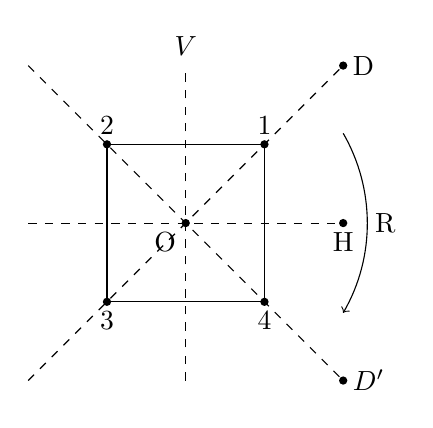
\begin{tikzpicture} 
\draw (-1, -1) rectangle (1,1);
\draw[dashed] (-2,0) -- (2,0); 
\draw[dashed] (-2,-2) -- (2,2); 
\draw[dashed] (0,-2) -- (0,2) node [above]{$V$}; 
\draw[dashed] (-2,2) -- (2,-2);
\draw[->] (2, 1.14) arc (30:-30:2.28);
\coordinate (A) at (0,0);
\fill(A) circle (1.5pt) node[below left]{O};
\coordinate (A) at (1,1);
\fill(A) circle (1.5pt) node[above]{1};
\coordinate (A) at (-1,1);
\fill(A) circle (1.5pt) node[above]{2};
\coordinate (A) at (-1,-1);
\fill(A) circle (1.5pt) node[below]{3};
\coordinate (A) at (1,-1);
\fill(A) circle (1.5pt) node[below]{4};
\coordinate (A) at (2,2);
\fill(A) circle (1.5pt) node[right]{D};
\coordinate (A) at (2,0);
\fill(A) circle (1.5pt) node[below]{H};
\coordinate (A) at (2,-2);
\fill(A) circle (1.5pt) node[right]{$D'$};
\node[right] (R) at (2.28, 0) {R};
\end{tikzpicture}
\caption{}\label{figure001060101}
\end{figure}


由计算表明$RH=D\neq HR$,由此我们顺便得到这里所说的“乘法”一般不满足交换律!但是它满足结合律,我们在\ref{section0010602}中将看到这一点。

读者计算正方形对称的其他乘积(\ref{section0010604}的表1中给出的一个完整的乘法表)是有意义的。当你做完这些乘积之后将会发现,一般地,逐次地把任意两个对称乘起来便得到第三个对称,但有个例外,例如,当$R$和$R'$相乘时,就会看到它的积是一个使正方形每个点都保持原来位置的运动,这就是所谓的“恒等”运动$I$. 这通常不被非数学家认为是对称;尽管如此,为了能使所有的对称两两相乘,我们还是把$I$看作一个(退化的)对称。

一般地,根据定义,几何图形的对称是图形上的点保持距离不变的一一变换。容易看出,正方形的任意对称一定把顶点1变换到四个可能的顶点之一,而且对每个这样的选择正好有两个对称,于是总共只有八个对称,就是我们已经列出来的那些。

不仅正方形,而且每个正多边形和正多面体(例如立方体和正二十面体)都存在有趣的对称群,可以用上面概述的出等方法找到。

类似的,很多装饰品有有趣的对称。例如我们考虑一个无限长的装饰图案

\begin{center}
\begin{tikzpicture} 
\draw[->] (0,0) -- (1,0); 
\draw (1,0) -- (2,0); 
\draw[->] (2,0) -- (3,0); 
\draw (3,0) -- (4,0); 
\draw[->] (4,0) -- (5,0); 
\draw (5,0) -- (6,0); 
\draw[->] (6,0) -- (7,0); 
\draw (7,0) -- (8,0); 
\end{tikzpicture}
\end{center}

在这个图案中,箭头是沿着直线以一英寸间隔均匀分布的。这个图形的三个简单的对称是:$T$, 向右平移一英寸;$T'$,向左平移一英寸;$H$,图形关于水平轴反射。其他对称(事实上是一切对称)可以由这三个对称反复相乘而得到。

\begin{problemset}
\item 计算$HV, HD', D'H, R'D', D'R', R'R''$.

\item 在“箭头”装饰图案中,描述对称$TH$和$HT$.

\item 列出等边三角形的所有对称,并计算五种具有代表性的乘积。

\item 列出普通矩形的所有对称,并计算它们的所有乘积。

\item 正四面体有多少对称? 正八面体有多少对称?画图说明。

\item 证明:正文中的装饰图案的任意对称可通过$H$, $T$和$T'$反复相乘而得到。

\end{problemset}



\section{变换群}\label{section0010602}
对称代数可以推广到无论什么元素的任意集合$S$的一一变换。虽然常常把集合$S$看作“空间”(例如平面或球),把$S$的元素看作“点”,并且把双射看作$S$的相对于适当性质的“对称”,然而在任何情况下,$S$的双射还满足一些非平凡的代数定律。

为了理解这些定律,我们必须清楚地记住\ref{section0010111}中给出的关于函数、单射、满射和双射的定义。为了重新解释它们,我们给出一些新的例子。同\ref{section0010111}一样,我们通常用缩写记号$xf$代替$f(x)$(读作“$x$通过$f$的变换”),用$xg$代替$g(x)$,等等。

函数$f(x)=e^{2\pi{}ix}$把实数域$\mathbb{R}$映入复数域$\mathbb{C}$,它的值域(像)是单位圆。类似的,$g(z)=|z|$是函数$g:\mathbb{C} \to \mathbb{R}$,它的像是所有非负实数的集合。

再有,考虑下列整数环$\mathbb{Z}$到自身的函数$\phi_0:\mathbb{Z} \to \mathbb{Z}$和$\psi_0:\mathbb{Z} \to \mathbb{Z}$:
\[
n\phi_0 = 2n, m\psi_0 = \left\{
\begin{aligned}
\frac{m}{2}, & \quad m \text{为偶数},\\
0,&\quad m \text{为奇数}.
\end{aligned}
\right.
\]
根据乘法消去律,$\phi_0$是一一的;然而它的值域仅由偶数组成,所以$\phi_0$没有把$\mathbb{Z}$变换到$\mathbb{Z}$上。另一方面, $\psi_0$不是一一的,这因为所有奇数都映射到零,但是它把$\mathbb{Z}$映到$\mathbb{Z}$上,于是$\psi_0$是满射, 而不是单射。

我们现在转到变换代数。具有相同的定义域$S$和相同的取值域$T$的两个变换$\phi:S \to T$和$\phi':S \to T$,如果它们作用到$S$的每一点上都有相同的效果,则称它们相等,即

\begin{gather}\label{equ001060201}
\phi = \phi'\text{的意思是},\text{对每个}p \in S, p\phi = p\phi'.
\end{gather}

再定义两个变换$\phi$和$\psi$的乘积或合成$\phi\psi$为它们相继作用的结果,先$\phi$后$\psi$,然而这里应假定$\phi$的取值域是$\psi$的定义域,换句话说,如果
\[
\phi: S \to T, \psi: T \to U,
\]
那么$\phi\psi$是由等式
\begin{gather}\label{equ001060202}
p(\phi\psi) = (p\phi)\psi
\end{gather}
给出的由$S$到$U$中的变换,式中规定$\phi\psi$作用到任意点$p \in S$, 特别是,$S$(到自身)的两个变换的乘积总是可以定义的。我们现在只考虑这种情况,只要假定所包含的乘积有定义,下面证明的恒等式几乎所有都可以用于一般情况。

变换的乘法适合

\textbf{结合律}
\[
(\phi\psi)\theta = \phi(\psi\theta),
\]

这里假定所包含的乘积都有定义,直观上这是显然的:$(\phi\psi)\theta$和$\phi(\psi\theta)$两者都是按照先$\phi$后$\psi$最后$\theta$的顺序作用的。正式地,对每个$p \in S$,我们有
\[
p[\phi(\psi\theta)] \mathop{=}_{\phi(\psi\theta)}(p\phi)(\psi\theta) \mathop{=}_{\psi\theta} [(p\phi)\psi]\theta \mathop{=}_{\phi\psi} [p(\phi\psi)]\theta \mathop{=}_{(\phi\psi)\theta} p[(\phi\psi)\theta],
\]
这里每步都依赖于乘法的定义(\ref{equ001060202}),也就是把定义(\ref{equ001060202})用到与每步相对应的等号下面标出的乘积上。根据变换相等的定义(\ref{equ001060201}),这就证明了结合律$\phi(\psi\theta)=(\phi\psi)\theta$.

集合$S$上的恒等变换$I = I_{S}$是使$S$上每个点保持固定的变换$I:S \to S$。代数上,这可叙述成等式
\begin{gather}\label{equ001060203}
pI = p, \text{对每个}p \in S.
\end{gather}
从上面的定义,直接推出
\textbf{同一律}
\[
I\phi = \phi{}I = \phi, \text{对一切}\phi.
\]
为了验证这一点,我们注意,对所有的$p$,有$p(I\phi) = (pI)\phi = p\phi$,类似的,$p(\phi{}I) = (p\phi)I = p\phi$.

现在回到前面定义在集合$Z$上的特殊变换$\phi_0$和$\psi_0$,并计算它们的乘积。显然
\[
m\psi_0\phi_0 = \left\{
\begin{aligned}
m, &\quad \text{当m为偶数},\\
0, &\quad \text{当m为奇数}.
\end{aligned}
\right.
\]
因此$\psi_0\phi_0 \neq I$。另一方面,对一切$m \in \mathbb{Z}$, 有$m\phi_0\psi_0 = m$,因此$\phi_0\psi_0 = I$.于是我们称$\psi_0$是$\phi_0$的右逆元素(而不是左逆元素)。

一般地,如果变换$\phi:S \to S$和$\psi:S \to S$具有$\phi\psi = I: S \to S$,那么称$\phi$是$\psi$的左逆怨怒是,而$\psi$是$\phi$的右逆元素。这些定义同以前定义的是“一一映入的(单射)”和“映上的(满射)”等概念有密切关系。

\begin{theorem}{}{thm001060201}
变换$\phi:S \to S$是一一的当且仅当它有右逆元素,$\phi$是映上的当且仅当它有左逆元素。
\end{theorem}

\begin{proof}
如果$\phi$有右逆元素$\psi$,$\phi\psi = I$,并且$p\phi = p'\phi$,那么
\[
p = p(\phi\psi) = (p\phi)\psi = (p'\phi)\psi = p'(\phi\psi) = p'.
\]
于是由$p\phi = p'\phi$可推出$p=p'$,因此$\phi$是一一的。类似的,如果$\phi$有左逆元素$\psi'$,则$\psi'\phi = I$.因此$S$中的任何元素$q$都可写成
\[
q = qI = q(\psi'\phi) = (q\psi')\phi,
\]
这表明$q$是某一点$p = q\psi'$的$\phi-$像。因此$\phi$是映上的。

反过来,已知任意$\phi:S \to S$,我们首先如下构造第二个变换$\psi:S \to S$. $S$中有一些点,其中每个点$q$是$S$的一个或多个点$p$在$\phi$之下的像。对每个点$q$,在这些点$p$中任意选出一个点作为像$q\psi$,那么,对形为$p\phi$的任何一个$q$,有
\[
q(\psi\phi) = (q\psi)\phi = p\phi = q.
\]
再令$\psi$随便按什么方式映射$S$中其余的点$q$,譬如说映射到(非空)集合$S$的某个固定点上。

现在,如果$\phi$是映上的,那么每个$q$都有形式$p\phi$,因此$\psi\phi=I$,所以$\phi$有$\psi$作为它的左逆元素。另一方面,如果$\phi$是一对一的,那么, 对每个$p$,$(p\psi)\phi$一定是唯一的$p$,即上面所说的$q = p\phi$中的$p$。因此$\phi\psi=I$,所以$\psi$是$\phi$的右逆元素,如断言所述。
\end{proof}

\textbf{注}\quad 微积分学中函数记号$y = \phi(x)$暗示记成$y = \phi{x}$, 而前面我们写成$y = x\phi$;按照这种记号,$\phi$和$z = \psi(y)$的合成自然写成$z = (\psi\phi)x$,它是作为$z = \psi(\phi(x))$的缩写记号,并代替$z = x\phi\psi$.因此$\psi\phi$的意思是“先执行$\phi$,后执行$\psi$”,而右逆元素和左逆元素的概念应相互对换。虽然上述两种记号用任何一种都是可以的,但是一定要避免他们之间的混淆。然而,双边逆元素的意思保持不变,正如下面推论所述。

\begin{corollary}{}{coro001060201}
变换$\phi:S \to S$是双射当且仅当它既有右逆元素又有左逆元素。如果$\phi$是双射,那么$\phi$的任意右逆元素等于$\phi$的任意左逆元素。
\end{corollary}

事实上,如果$\phi$有右逆元素$\theta$和左逆元素$\psi$,那么
\[
\theta = I\theta = (\psi\phi)\theta = \psi(\phi\theta) = \psi{}I = \psi.
\]

把变换$\phi:S \to S$的(双边)逆元素定义为满足

\textbf{逆律}
\[
\phi\phi^{-1} = \phi^{-1}\phi = I
\]
的任意变换$\phi^{-1}$.这些等式也表明$\phi^{-1}$是$\phi$的(双边)逆元素,因此进一步有
\begin{corollary}{}{coro001060202}
变换$\phi:S \to S$是双射当且仅当$\phi$有(双边)逆元素$\phi^{-1}$。如果$\phi$是双射,那么$\phi$的任何两个逆元素是相等的,并有
\begin{gather}\label{equ001060204}
(\phi^{-1})^{-1} = \phi.
\end{gather}
\end{corollary}

这个推论后面将要用到。它可以直接证明,因为$\phi^{-1}$只不过是这样一个变换,它把$S$的每个点$q = p\phi$变回原来唯一的点$p$.在$S$是有限的特殊情况下,$\phi$是一一的当且仅当$\phi$是映上的,因此在这种情况下左逆元素和右逆元素的更细致的讨论是没有意义的。

对于集合$S$到另一个集合$T$的函数$\phi: S \to T$来说,定理\ref{thm:thm001060201}及其推论以及它们的证明也都成立。我们只需注意,左逆元素$\psi$或者右逆元素$\theta$是第二个集合$T$到集合$S$中的变换,并注意
\[
\psi\phi = I_T: T \to T, \quad \phi\theta = I_S:S \to S.
\]
这里$I_S$和$I_T$分别是$S$和$T$上的恒等变换。

我们现在准备定义变换群这一重要概念。“空间”$S$上的变换群是指满足下列条件的把$S$映上$S$的一一变换$\phi$组成的任意集合$G$:
\begin{enumerate}
\item[(i)]$S$的恒等变换在$G$中;
\item[(ii)]如果$\phi$在$G$中,则它的逆元素也在$G$中;
\item[(iii)]如果$\phi$和$\psi$在$G$中,则它们的积也在$G$中。
\end{enumerate}

\begin{theorem}{}{thm001060202}
任意空间$S$到自身的所有双射所组成的集合$G$是一个变换群。
\end{theorem}

\begin{proof}
因为$II=I$,$S$上的恒等变换$I$是双射,因此$I$在集合$G$中,上面的条件(I)满足。如果$\phi$在$G$中,由前面的推论\ref{cor:coro001060202}得$\phi^{-1}$也是双射,因此它同样在$G$中,条件(II)满足。最后,任意两个把$S$映上$S$的一一变换$\phi$和$\psi$,它们的乘积有逆元素,因为根据假设
\begin{gather*}
(\phi\psi)(\psi^{-1}\phi^{-1}) = \phi(\psi\psi^{-1})\phi^{-1} = \phi{}I\phi = \phi\phi^{-1} = I,\\
(\psi^{-1}\phi^{-1})(\phi\psi) = \psi^{-1}(\phi^{-1}\phi)\psi = \psi^{-1}I\psi = \psi^{-1}\psi = I,
\end{gather*}
因此$\phi\psi$也是双射,并且有逆元素
\begin{gather}\label{equ001060205}
(\phi\psi)^{-1} = \psi^{-1}\phi^{-1}.
\end{gather}
口头上说就是,乘积的逆元素等于逆元素颠倒次序相乘。
\end{proof}

有限集$S$到自身的双射通常称为$S$的置换。$n$个元素的所有置换组成的群称为$n$次对称群;显然它包含$n!$个置换,这因为第一个元素的像$k_1$,可以有$n$种方式选取,然后,第二个元素的像可从去掉$k_1$剩下的元素中以$n-1$种方法选取,等等。

\begin{problemset}
\item\label{exer001060201} 在正方形对称群中计算$VD,(VD)R'', DR'', V(DR'')$.

\item 类似习题\ref{exer001060201},计算$HR, R'(HR), R'H, (R'H)R$.

\item 设$S$由所有实数组成(或由直线上的所有点$x$组成),所考察的变换具有形式$x\phi = ax+b$.在下列各种情况中,以所指定类型的$a$和$b$为系数的所有可能的变换$\phi$组成的集合,哪些是变换群,并给出证明。
\begin{enumerate}
\item[(a)]$a$和$b$是有理数;
\item[(b)]$a=1$, $b$是奇数; 
\item[(c)]$a=1$, $b$是正整数或零;
\item[(d)]$a=1$, $b$是偶数;
\item[(e)]$a$是整数,$b=0$;
\item[(f)]$a \neq 0$,$a$和$b$是实数;
\item[(g)]$a \neq 0$, $a$是整数,$b$是实数;
\item[(h)]$a \neq 0$, $a$是实数,$b$是整数;
\item[(i)]$a \neq 0$, $a$是整数,$b$是无理数;
\item[(j)]$a \neq 0$, $a$是有理数,$b$是实数。
\end{enumerate}
在这些变换群中,哪些群的乘法满足交换律?

\item 找出恰有三个“点”的“空间”$S$上的所有变换,共有多少个变换?其中有多少是一一变换?

\item 证明:所有正整数的集合上的变换$n \mapsto n^2$没有左逆元素。并列出两个明显的右逆元素。

\item 列出正文中定义的变换$\psi_0: \mathbb{Z} \to \mathbb{Z}$的两个不同的左逆元素,并列出$\phi_0$的两个不同的右逆元素。

\item 证明:如果$\phi$和$\psi$二者都有右逆元素,那么$\phi\psi$也有右逆元素。

\item 对于正方形对称群,计算$[R^{-1}(VR)]^{-1}[(R^{-1}D)R]$.

\item对正方形对称群。解方程$RXR'=D$.

\item 在正方形对称群中,验证
\[
(RH)^{-1} = H^{-1}R^{-1} \neq R^{-1}H^{-1}.
\]

\item 求出矩形每个对称的逆元素,并验证公式(\ref{equ001060205})。

\item 证明:如果$\phi_1,\phi_2,\cdots, \phi_n$是一一的,那么$\phi_1\phi_2\cdots\phi_n$也是一一的,且有逆元素
\[
(\phi_1\phi_2\cdots\phi_n)^{-1} = \phi_n^{-1}\cdots\phi_2^{-1}\phi_1^{-1}.
\]

\item 证明:对任意$\phi:S \to S$。由定理\ref{thm:thm001060201}证明的第二部分所构造的变换$\psi$满足$\phi\psi\phi = \phi$.

\item 证明:具有唯一右逆元素或唯一左逆元素的变换$\phi:S \to S$,必是$S$到$S$上的一一变换。


\end{problemset}


\section{其他例子}\label{section0010603}
立方体的所有对称构成另一个有趣的群。用几何语言来说,这些对称是保持立方体上距离不变的一一变换。它们被称为“等距变换”,共有48个。为了说明这一点,我们注意到,任意一个初始顶点可以变换到八个顶点的中任意一点。任意顶点的变换固定之后,这个顶点的三个相邻顶点可以有六种方式进行排列,于是给出$6 \cdot 8 = 48$种可能性。当一个顶点和它的三个相邻顶点的位置确定时,立方体上任何一点的位置也就固定下来,所以整个对称就知道了。因此立方体恰有48个对称。它们中间很多都具有特殊的几何性质,例如,其中一个对称是把立方体的每个点反射成对径点。

包含着无穷多个变换的一个熟悉的群是所谓欧几里得群。这个群由平面的所有“等距变换”组成,或者用初等几何的语言来说,在这些变换下,平面同自身是全等的。这个群由平移、刚体旋转和反射的乘积组成。我们将在第\ref{chapter00109}章详细讨论它。

另一个群是由空间的所有“相似变换”组成,即由那些使一切距离扩大常数$k$($k>0$,称为比例因子)倍的一一变换组成。任意球面变为自身的所有刚体运动又构成一个群。使平面上正六边形网络保持不变的所有“等距变换”构成另一个有趣的群。

再有,一条橡皮绳沿一直线摆放着,绳的两端分别固定在$P,Q$两点,它可以沿着这条直线以很多种方式变形。所有这些变形构成一个群(通常称为线段$PQ$的同胚群)。

一般地说,任意集合的一一变换,如果保持集合中元素的某个或某些任意给定的性质,那么这些一一变换构成一个群。克莱茵(Felix Klein)(Erlanger纲领, 1872)雄辩地描述了,不同的几何分支可以看作是研究相应空间的那些在适当的变换群下保持不变的性质。例如,欧几里得几何是研究空间的那些在所有等距变换下保持不变的性质,拓扑学是研究空间的那些在所有同胚变换下保持不变的性质。类似的,射影几何和仿射几何分别研究空间在射影群和仿射群下保持不变的性质。射影群和仿射群的定义将在第\ref{chapter00109}章给出。

\begin{problemset}
\item\label{exer001060301} 描述带有六个等间隔辐条的车轮的全部对称。

\item 描述一个顶点固定的立方体的六个对称。

\item 设$S, T$是立方体关于平面的反射,这两个平面分别平行于立方体的两个不同的侧面。描述$ST$的几何意义。

\item\label{exer001060304} 描述一些把图2的正六边形网络变到自身的平面等距变换。

\item 对正方形网络作习题\ref{exer001060304}。你能数出所有这样的变换吗(这是困难的)?

\item 对正三角形网络作习题\ref{exer001060304}。并说明这些变换与习题\ref{exer001060301}的变换群的关系。

\item 对下述几种情况作习题\ref{exer001060304}:
\begin{enumerate}
\item[(a)]无限圆柱体.
\item[(b)]有限圆柱体,
\item[(c)]圆柱螺旋线,即一条围绕柱面并与圆柱轴线成定角的螺旋线。
\end{enumerate}

\item 证明:所有变换$x \mapsto x'=\frac{ax+b}{cx+d}$(其中系数$a,b,c,d$在任意域$F$中,并且$ad-bc=1$)组成一个群,这些变换作用在由域$F$的全体元素和符号元素$\infty$组成的集合上。
\end{problemset}


\section{抽象群}\label{section0010604}
变换群绝不是其乘法满足\ref{section0010602}中所说的结合律、同一律和逆律的唯一系统。例如,任意域(如有理数域,实数域和复数域)的全体非零元素都满足这些定律。因为任意两个非零元素的乘积是一个非零元素;结合律成立;域的单位元素1满足同一律,并且$\frac{1}{x} = x^{-1}$满足逆律。

类似的,任意整环的全体元素(这次包括零)在加法运算之下满足上述三个定律。例如,任意两个元素有唯一确定的和;加法满足结合律;对于加法运算,零满足同一律,$-x$满足逆律。换句话说,任意整环的全体元素在加法之下构成一个群。

为方便起见,我们引进包含上述和其他一些例子的群的抽象概念。

\begin{definition}{群(Group)}{def001060401}
具有二元运算的元素集合$G$, (i)运算满足结合律;(ii)有一个满足同一律的单位元素;(iii)对每个元素$a$, 有元素$a^{-1}$(称为$a$的逆)满足逆律,则这个集合$G$称为群。
\end{definition}

我们可以不提变换,用许多方式抽象地给出群的定义,这样定义的群常常称为抽象群。

在讨论抽象群的时候,元素用小写拉丁字母$a,b,c,\cdots$来表示。乘积记号“$ab$”通常用来表示$G$的两个元素$a$和$b$在群的运算之下而得的结果,但是其他记号,像“$a+b$”和“$a \circ b$”也同样适用。在乘积记号中,用“$e$”表示单位元素,定义群的三个定律变为
\begin{enumerate}
\item[结合律] $a(bc) = (ab)c$,对一切$a,b,c$.
\item[同一律] $ae = ea = a$, 对一切$a$.
\item[逆律]$aa^{-1} = a^{-1}a = e$, 对每个$a$和某个$a^{-1}$.
\end{enumerate}

其运算满足交换律的群称为交换群或阿贝尔群。利用这个概念我们可以把域的定义简化如下。

\begin{definition}{域}{def001060402}
集合$F$满足下列条件时称为域,$F$在两个唯一确定的二元运算---加法和乘法之下是封闭的,并有
\begin{enumerate}
\item[(i)]在加法之下,$F$是具有单位元素零的交换群;
\item[(ii)]在乘法之下,$F$中非零元素构成交换群;
\item[(iii)]分配律成立:$a(b+c) = ab+ac$.
\end{enumerate}
\end{definition}

为证明这个定义同\ref{section0010201}中给出的定义是等价的,我们注意,这里给出的公设,除了含有因子零的乘法结合律外,包含前面对域所描述的一切公设。这可以详细地验证。

第\ref{chapter00101}、\ref{chapter00102}章的第一节中的一些结果现在将表现为下面关于群的定理的推论。
\begin{theorem}{}{thm001060403}
在任意群中,$xa=b$和$ay=b$有唯一解,分别为$x=ba^{-1}$和$y=a^{-1}b$。因此由$ca=da$可推出$c=d$,同样由$ac=ad$克推出$c=d$(消去律)。
\end{theorem}

\begin{proof}
如果$a^{-1}$是在逆律中确定的元素,显然,$(ba^{-1})a=b(a^{-1}a)=be=b$. 类似的,$a(a^{-1}b)=b$。反过来,由$xa=b$可推出$x=xe=xaa^{-1}=ba^{-1}$,同样地,由$ay=b$可推出$y=a^{-1}b$.
\end{proof}

注意,在这个证明中并没有假定$a^{-1}$是满足$xa=e$的唯一的元素。但$a^{-1}$确是唯一的,这是因为,若$xa=e$,则
\[
x=xe=x(aa^{-1})=(xa)a^{-1}=ea^{-1}=a^{-1}.
\]
类似地,$a^{-1}$是使得$ay=e$的唯一元素。

因为根据定理\ref{thm:thm001060403}, 在任意群$G$中方程$ex=e$和$ay=e$有唯一解分别为$x=e$和$y = a^{-1}$,因此,我们得到
\begin{corollary}{}{coro001060401}
群有唯一的单位元素,并且对每个元素$a$有唯一的逆$a^{-1}$.
\end{corollary}

\begin{theorem}{}{thm001060404}
前面所述的群的定义中,同一律和逆律可以用较弱的形式来代替。

\textbf{左同一律}\quad 对所有的元素$a$,存在某元素$e$,满足$ea = a$.

\textbf{左逆律}\quad 对给定的元素$a$,存在某元素$a^{-1}$,满足$a^{-1}a = e$.
\end{theorem}

\begin{proof}
如果这些弱的定律成立,则左消去律也成立,即由$ca = cb$可推出$a=b$。因为我们只须用$c^{-1}$左乘等式$ca=cb$的两边,再用结合律得到$(c^{-1}c)a = (c^{-1}c)b$,这就是$ea=eb$,故得$a=b$.

给出的这个左单位元素也是右单位元素,这是因为
\[
a^{-1}ae = ee = e = a^{-1}a
\]
再根据左消去律,因此对所有的$a$,有$ae=a$. 最后,左逆元素也是右逆元素,因为由于左单位元素也是右单位元素,则有
\[
a^{-1}(aa^{-1}) = (a^{-1}a)a^{-1} = ea^{-1}=a^{-1} = a^{-1}e,
\]
现在再用左消去律,得$aa^{-1}=e$。这就完成了我们的证明。
\end{proof}

还有很多其他的群公设系统,常用的一个是按照除法的可能性来建立的,如下所述:
\begin{theorem}{}{thm001060405}
如果$G$是一个非空集合,在满足结合律的乘法之下是封闭的,对于这个集合所有的方程$xa=b$和$ay=b$在$G$中有解$x$和$y$,那么$G$是一个群。
\end{theorem}

证明留做习题。

除了对任意群$G$把有关乘法的代数定律系统化以外,当$G$的元素有限时,我们还可以用“乘法表”的形式给出$G$中任意两个元素乘积的特殊构成法则。这个乘法表是一些元素的正方形阵列,表的最左一列和最上一行列出群的所有元素。表中对应着最左列上的$a$和最上行的$b$的那个元素是乘积$ab$(按此次序)。

为举例说明,我们在表\ref{table001060401}中绘制了正方形对称群的乘法表。这个表的计算可以按照\ref{section0010601}中证明的$HR=D'$和$RH=D$的模式来进行。其他方法将在\ref{section0010606}中描述。
\begin{table}
\caption{正方形对称群}\label{table001060401}
\begin{center}
\begin{tabular}{|c|c|c|c|c|c|c|c|c|}
\hline
&$I$ & $R$ & $R'$ & $R''$ & $H$ & $V$ & $D$ & $D'$\\ \hline
$I$ & $I$ & $R$ & $R'$ & $R''$ & $H$ & $V$ & $D$ & $D'$ \\ \hline
$R$ & $R$ & $R'$ & $R''$ & $I$ & $D$ & $D'$ & $V$ & $H$ \\ \hline
$R'$ & $R'$ & $R''$ & $I$ & $R$ & $V$ & $H$ & $D'$ & $D$ \\ \hline
$R''$ & $R''$ & $I$ & $R$ & $R'$ & $D'$ & $D$ & $H$ & $V$ \\ \hline
$H$ & $H$ & $D'$ & $V$ & $D$ & $I$ & $R'$ & $R''$ & $R$ \\ \hline
$V$ & $V$ & $D$ & $H$ & $D'$ & $R'$ & $I$ & $R$ & $R''$ \\ \hline
$D$ & $D$ & $H$ & $D'$ & $V$ & $R$ & $R''$ & $I$ & $R'$ \\ \hline
$D'$ & $D'$ & $V$ & $D$ & $H$ & $R''$ & $R$ & $R'$ & $I$ \\ \hline
\end{tabular}
\end{center}
\end{table}

关于群的大部分性质可以直接从表中看到。例如,单位元素的存在表明,某一行和相应的列一定分别是顶头一行和最左边一列的复制品。方程$ay=b$可解意味着$a$所在的那一行一定包含元素$b$;因为解是唯一的,所以$b$在这一行中只能出现一次。一个群是交换群当且仅当它的乘法表关于主对角线(即左上角到右下角的联线)是对称的。遗憾的是,结合律不容易从这个表中直观地看出。

\begin{problemset}
\item 设$a,b,c$是群的固定元素,证明方程$xaxba=xbc$有唯一解。

\item 证明:在$2n$和元素的群中,除单位元素外还存在一个元素同它的逆相等。

\item 全体正实数在加法下构成一个群吗?在乘法下构成群吗?全体偶数在加法下构成群吗?全体奇数呢?为什么?

\item 在模11整数域$\mathbb{Z}_{11}$中,下列集合中哪些在乘法下构成群:
\begin{enumerate}
\item[(a)] $(1,3,4,5,9)$,
\item[(b)] $(1,3,5,7,8)$,
\item[(c)] $(1, 8)$,
\item[(d)] $(1, 10)$.
\end{enumerate}

\item 证明:含有四个元素或少于四个元素的群一定是阿贝尔群。(提示:$ba$是$e, a, b, ab$中的一个,显然的情形除外。)

\item 证明:如果在一个群中$xx=x$,则$x=e$.

\item 下列乘法表描述一个群吗?
\begin{table}
\begin{minipage}{0.45\textwidth}
\centering
\begin{tabular}{|c|c|c|c|c|}
\hline
&$a$ & $b$ & $c$ & $d$ \\ \hline
$a$ & $b$ & $d$ & $a$ & $c$ \\ \hline
$b$ & $d$ & $c$ & $b$ & $a$ \\ \hline
$c$ & $a$ & $b$ & $c$ & $b$ \\ \hline
$d$ & $c$ & $a$ & $d$ & $a$ \\ \hline
\end{tabular}
\end{minipage}
\begin{minipage}{0.45\textwidth}
\centering
\begin{tabular}{|c|c|c|c|c|}
\hline
&$a$ & $b$ & $c$ & $d$ \\ \hline
$a$ & $a$ & $b$ & $c$ & $d$ \\ \hline
$b$ & $b$ & $a$ & $d$ & $c$ \\ \hline
$c$ & $c$ & $d$ & $a$ & $a$ \\ \hline
$d$ & $d$ & $c$ & $b$ & $b$ \\ \hline
\end{tabular}
\end{minipage}
\end{table}

\item 证明:\ref{section0010102}中法则2(单位元),4(消去律),和6(逆元唯一性)在任意交换群中都成立。

\item 下列数集中哪一些是群?为什么?
\begin{enumerate}
\item[(a)] 所有有理数,在加法运算之下;在乘法运算之下;
\item[(b)] 所有无理数,在乘法运算之下;
\item[(c)] 所有绝对值为1的复数,在乘法运算之下;
\item[(d)] 所有绝对值为1的复数,在运算$z \circ z' = |z| \cdot z'$之下;
\item[(e)] 所有整数,在减法运算之下;
\item[(f)] 任意整环的全体单位(\ref{section0010306}),在乘法运算之下;
\end{enumerate}

\item 证明:下列公设系统描述一个阿贝尔群:
\begin{enumerate}
\item[(i)] 对一切$a,b,c$有$(ab)c = a(bc)$;
\item[(ii)]定理\ref{thm:thm001060404}的“左同一律”成立;
\item[(iii)]定理\ref{thm:thm001060404}的“左逆律”成立;
\end{enumerate}

\item 证明:如果对群$G$中所有元素有$x^2=e$,那么$G$是交换群。

\item 证明定理\ref{thm:thm001060405}。(提示:如果$ax=a$,那么$x$是右单位元素,并且任意右单位元素等于左单位元素。)

\item 设$S$是一个非空集合,在乘法运算之下是封闭的,并且满足$ab=ba$, $a(bc)= (ab)c$, 由$ax=ay$可推出$x=y$.
\begin{enumerate}
\item[(a)]证明:若$S$有限,则$S$是群。
\item[(b)]证明:若$S$有限或无限,则$S$可以嵌入一个群中。
\end{enumerate}

\end{problemset}




\section{同构}\label{section0010605}
考虑实数整环上的变换$x \mapsto \log{x}$.我们知道,当$x$在区间$0 < x < +\infty$上增加时, $\log{x}$就在区间$-\infty < x < +\infty$上连续增加;也就是说,这个对应是正实数系和全体实数系之间的一一对应(逆变换是$y \mapsto e^{y}$)。而且对所有的$x, y$,有$log{xy} = \log{x} + \log{y}$, 于是我们可以用相应的和的计算代替乘积的计算。事实上,这是对数主要的实际用途。

其次,设$\mathbb{Z}_3$是模3整数构成的域(\ref{section0010310}),并设$G$是等边三角形到自身的刚体旋转群。如果$I, R$和$R'$分别表示转过$0^{\circ}$,$120^{\circ}$和$240^{\circ}$的旋转,那么把整数同旋转联系起来的对应$0 \leftrightarrow I$, $1 \leftrightarrow R$, $2 \leftrightarrow R'$是一个把$\mathbb{Z}_3$中元素的和映射成$G$中相应旋转的乘积的双射。例如,考虑对应

\begin{equation*}
\begin{aligned}
1 + 2 \equiv 0 (\mod{3})\quad &\leftrightarrow &&RR' = I\\
2 + 2 \equiv 1 (\mod{3})\quad &\leftrightarrow &&R'R' = R
\end{aligned}
\end{equation*}

这些都是\ref{section0010112}中所谈到的“同构”一般概念的例子,这个概念对群来说比对整环更简单也更重要。
\begin{definition}{}{def001060501}
两个群$G$和$G'$之间的同构指的是它们元素之间保持群的乘法的双射$a \leftrightarrow a'$,即它满足, 若$a \leftrightarrow a'$和$b \leftrightarrow b'$,则$ab \leftrightarrow a'b'$.
\end{definition}

例如,在第一个例子中我们描述了正实数乘法群与实数加法群之间的同构,在第二个例子中,我们指出一个模3整数加法群与正三角形旋转对称群之间的同构。

类似的,映射$0 \mapsto 1$, $1 \mapsto 2$, $2 \mapsto 4$, $3 \mapsto 3$是模4整数加法群与模5非零整数乘法群之间的同构。通过比较模4整数加法群的加发表和模5非零整数乘法群的乘法表来验证这个结果是方便的。见表\ref{table001060502}和表\ref{table001060503}.
\begin{table}
\begin{minipage}{0.45\textwidth}
\centering
\caption{}\label{table001060502}
\begin{tabular}{c|cccc}
$+$ & $0$ & $1$ & $2$ & $3$ \\ \hline
$0$ & $0$ & $1$ & $2$ & $3$ \\
$1$ & $1$ & $2$ & $3$ & $0$ \\
$2$ & $2$ & $3$ & $0$ & $1$ \\
$3$ & $3$ & $0$ & $1$ & $2$ 
\end{tabular}
\end{minipage}
\begin{minipage}{0.45\textwidth}
\centering
\caption{}\label{table001060503}
\begin{tabular}{c|cccc}
$\times$ & $1$ & $2$ & $4$ & $3$ \\ \hline
$1$ & $1$ & $2$ & $4$ & $3$ \\
$2$ & $2$ & $4$ & $3$ & $1$ \\
$4$ & $4$ & $3$ & $1$ & $2$ \\
$3$ & $3$ & $1$ & $2$ & $4$ 
\end{tabular}
\end{minipage}
\end{table}

依次我们有,模4整数加法群同构于正方形旋转对称群。通过比较表\ref{table001060502}和表\ref{table001060401}(\ref{section0010604})的旋转部分可以验证,双射$0 \leftrightarrow I$, $1 \leftrightarrow R$, $2 \leftrightarrow R'$, $3 \leftrightarrow R''$是一个同构。

同构的概念很重要,因为它使我们认识到,完全不同的群从抽象群论的观点看可以看成同一个群。同构的群抽象地认为是同一个群(它们的差别仅在于它们元素符号的不同),这个事实可以在很多情况下看到。

例如,根据定义,两个有限群$G$和$G'$同构当且仅当通过适当的替换,从$G$的群表可以得出$G'$的群表,从\ref{section0010604}的倒数第二句可以得出,$G'$是阿贝尔群当且仅当$G$是阿贝尔群,也就是说,一个有限阿贝尔群的任何同构像是阿贝尔群,还有,在其他方面,同构的性质很像相等。

\begin{theorem}{}{thm001060506}
关系“群$G$同构于群$G'$”满足群之间的自反的,对称的和传递的关系。
\end{theorem}

\begin{proof}
自反性是显然的(每个群通过恒等变换同它自身同构)。对于对称性,设$a \leftrightarrow aT$是$G$和$G'$之间的任意同构对应,因为$T$是双射,所以$T$有逆元素$T^{-1}$,$T^{-1}$是$G'$到$G$上的同构。最后,如果$T$把$G$同构地映射到$G'$上,而$T'$把$G'$同构地映射到$G''$上,那么$TT'$就是$G$和$G''$之间的同构。
\end{proof}

值得注意的是,定理\ref{thm:thm001060506}及其证明对于整环之间的同构同样成立,而且对于任何类型的代数系统之间的同构也都成立。

\begin{theorem}{}{thm001060507}
在两个群同构之下,它们的单位元素相互对应,相应元素的逆元素相互对应。
\end{theorem}

\begin{proof}
方程$ax=a$的唯一解$e$对应到$a'x=a'$的唯一解$e$,因此单位元素相互对应。所以,$G$中方程$ax=e$的唯一解$a^{-1}$对应到$G'$中方程$a'x=e'$的唯一解$a'^{-1}$. 这就完成了证明。
\end{proof}

我们最后证明著名的凯莱(Cayley)定理,这个定理可被解释为是证明变换乘法有关公设的完备性。

\begin{theorem}{}{thm001060508}
任意抽象群$G$与一个变换群同构。
\end{theorem}

\begin{proof}
把由$G$的所有元素组成的“空间”上的每个变换$\phi_a: x \to xa = x\phi_a$同$G$的元素$a$联系起来。因为由$e\phi_a = e\phi_b$可推出$a=ea=eb=b$,所以$G$的不同元素对应着不同的变换,因为对所有的$x$,有
\begin{equation}\label{equ001060506}
x(\phi_a\phi_b) = (x\phi_a)\phi_b = (xa)\phi_b = (xa)b = x(ab) = x\phi_{ab},
\end{equation}
所以乘积$\phi_a\phi_b = \phi_{ab}$,因而所有$\phi_a$的集合$G'$包含任意两个变换,就一定包含它们的乘积。再有,因为对所有的$x$有$x\phi_e = xe = x$,所以$G'$包含单位元素。我们可以类似地证明,对所有的$a$, $(\phi_a)^{-1}$存在,并在$G'$中,实际上它就是$\phi_{a^{-1}}$, 因此$G'$是一个变换群,根据(\ref{equ001060506}),它与$G$同构。
\end{proof}

\begin{problemset}
\item\label{exer001060501} 下列群中,任意两个群都同构吗?
\begin{enumerate}
\item[(a)] 等边三角形的对称群;
\item[(b)] 正方形对称群;
\item[(c)] 正六边形的旋转群;
\item[(d)] 模6整数加法群。
\end{enumerate}

\item 与习题\ref{exer001060501}同样的问题。
\begin{enumerate}
\item[(a)] 正方形的旋转群;
\item[(b)] 矩形的对称群;
\item[(c)] 菱形(等边平行四边形)的对称群;
\item[(d)] 模13整数1,5,8,12的乘法群;
\item[(e)] 模12整数1,5,7,11的乘法群。
\end{enumerate}

\item (a)证明:“高斯整数”$m + n\sqrt{-1}$($m, n \in \mathbb{Z}$)的加法群同形为$2^n3^m$($m, n \in \mathbb{Z}$)的有理因子的乘法群同构。

(b)给出两个与矩形网络的变换群同构的群。

\item 非零实数构成的乘法群与所有实数构成的加法群同构吗?

\item 确定$\mathbb{Z}_4$的加法群与正方形的旋转群之间的所有同构。

\item\label{exer001060506} (a)列出正方形对称群与正方形四个顶点1,2,3,4上的变换群之间的同构。

(b)像定理\ref{thm:thm001060507}那样明显地指出,两个群中的逆元素在这个同构之下是如何对应的。

\item 对正六边形的旋转群做习题\ref{exer001060506}.

\item 列出与下列每个群同构的变换群,说明定理\ref{thm:thm001060508}
\begin{enumerate}
\item[(a)] 所有实数构成的加法群;
\item[(b)] 所有非零实数构成的乘法群;
\item[(c)] 模8整数加法群。
\end{enumerate}

\end{problemset}



\section{循环群}\label{section0010606}
在任意群中,元素$a$的整数幂$a^m$可以分别对正指数、零指数和负指数来定义。当$m>0$时,我们定义
\begin{equation}\label{001060607}
a^m = a\cdot a \cdots a (\text{m个因子}), a^0 = e, a^{-m} = (a^{-1})^m.
\end{equation}



\chapter{几何}\label{chapter00109}


